\documentclass[11pt,a4paper]{article}

% Canonical package preamble (duplicates removed).
\usepackage[a4paper,margin=1in]{geometry}
\usepackage[T1]{fontenc}
\usepackage[utf8]{inputenc}
\usepackage{lmodern,microtype,setspace}
\usepackage{amsmath,amssymb,amsfonts,mathtools}
\usepackage{booktabs,longtable,tabularx,array,multirow,makecell,adjustbox}
\newcolumntype{Y}[1]{>{\raggedright\arraybackslash}p{#1}}
\usepackage{graphicx,pdflscape,flafter,float}
\usepackage[table]{xcolor}
\usepackage{tikz,pgfplots}
\usetikzlibrary{arrows.meta,calc,positioning,shapes.geometric,fit,backgrounds}
\pgfplotsset{compat=1.18}
\usepackage{caption,subcaption}
\usepackage[numbers,sort&compress]{natbib}
\usepackage{hyperref}
\usepackage{cleveref}
\onehalfspacing
\setlength{\emergencystretch}{3em}
\definecolor{darkblue}{RGB}{30,60,110}
\definecolor{lightblue}{RGB}{235,243,250}
\hypersetup{colorlinks=true,linkcolor=darkblue,citecolor=darkblue,
    urlcolor=blue,pdftitle={From Parkinson's disease genome-wide association signals to testable mechanistic hypotheses: an integrated GWAS2Mech analysis},
    pdfauthor={Muhammad Muneeb and Enric Glabb}}
\setcounter{tocdepth}{3}

\title{
    \textbf{From Parkinson's disease genome-wide association signals to testable mechanistic hypotheses}\\[0.3cm]
    \large An integrated GWAS2Mech analysis
}

\author{Muhammad Muneeb\textsuperscript{1} \quad Enric Glabb\textsuperscript{1}\\[0.4em]
\small \textsuperscript{1}University of Luxembourg, Luxembourg}

\date{}

\begin{document}

\maketitle

\begin{abstract}
\noindent\textbf{Background:} Genome-wide association studies identify loci associated with Parkinson's disease, but linkage disequilibrium and context-dependent gene regulation complicate the assignment of causal variants, effector genes, and downstream biological processes. We developed GWAS2Mech to integrate statistical fine-mapping with functional annotation, molecular quantitative trait locus (QTL) colocalisation, external benchmarking, pathway and protein-association analyses, and public perturbation data.

\noindent\textbf{Methods:} Seventeen European-ancestry GWAS datasets for Parkinson's disease and related phenotypes were harmonised to GRCh38 and analysed with a 1000 Genomes 30$\times$ European linkage disequilibrium reference. Associated loci underwent SuSiE-RSS fine-mapping, variant annotation, and molecular-QTL colocalisation. Candidate genes were compared with Open Targets, tested for pathway and protein-association enrichment, and linked to source-matched single-cell perturbation signatures. Each final record retained its study, locus, variant, molecular phenotype, pathway, experimental context, and unresolved evidence fields.

\noindent\textbf{Results:} Eight studies yielded 69 nominal 95\% credible sets. Cross-layer quality control supported 24 candidate genes for downstream analysis. Public perturbation resources contained usable contrasts for eight candidates, and 14 gene--pathway--experiment records passed the exploratory gene-set permutation filter. Only one record linked the same genetically prioritised pathway gene to the corresponding perturbation response: \textit{NSF} and Golgi vesicle transport. \textit{KANSL1} perturbations produced respiration-, mitochondrial-, and cytoskeleton-related transcriptional signatures, but these terms lacked same-gene pathway-driver support in the genetic enrichment analysis.

\noindent\textbf{Conclusions:} GWAS2Mech converts heterogeneous association evidence into traceable, testable mechanistic hypotheses while preserving uncertainty across evidence layers. The analysis prioritised \textit{NSF}-related vesicular transport for experimental follow-up, but did not establish allele-to-pathway causal direction, a clinically validated mechanism, or a therapeutic effect.
\end{abstract}

\noindent\textbf{Keywords:} Parkinson's disease; genome-wide association study; fine-mapping; molecular QTL; colocalisation; pathway analysis; protein association; genetic perturbation

\clearpage
\tableofcontents

\clearpage

\section{Introduction}
\label{sec:introduction}

Genome-wide association studies (GWAS) have identified reproducible Parkinson's disease (PD) susceptibility loci, yet most associated variants do not directly reveal the affected gene or biological process. Correlated variants within linkage disequilibrium blocks can support several plausible signals, and regulatory effects may differ by tissue, cell type, transcript, or molecular phenotype. Statistical fine-mapping can reduce the set of candidate variants, but a credible set is a probabilistic summary rather than proof of causality \cite{Wang2020,Zou2022}.

Mechanistic interpretation therefore requires evidence from several complementary sources. Variant annotations describe predicted molecular consequences and regulatory context; molecular quantitative trait loci (QTLs) connect genetic variation to measured molecular phenotypes; and colocalisation tests whether disease and molecular associations are compatible with a shared signal. Resources such as Open Targets integrate fine-mapping, locus-to-gene, functional-genomic, and disease evidence, providing an external reference for evaluating gene prioritisation \cite{Mountjoy2021,OpenTargets2026Release}.

Pathway and protein-association analyses can place prioritised genes within biological systems, but enrichment and network connectivity do not demonstrate causal mediation. Perturbation experiments provide a distinct evidence layer by testing whether changing a candidate gene is accompanied by a transcriptional response in a defined cellular context. Public single-cell perturbation collections improve access to these experiments, although differences in model system, guide design, replication, and preprocessing constrain cross-study interpretation \cite{Peidli2024scPerturb,Squair2021FalseDiscoveries}.

This study applied GWAS2Mech to 17 European-ancestry GWAS datasets for Parkinson's disease and related phenotypes. The objectives were to identify statistically supported loci and variants, prioritise candidate effector genes through molecular evidence, compare those assignments with Open Targets, and determine which genetically enriched pathways had corresponding public perturbation evidence. The analysis was designed as a provenance-preserving hypothesis-prioritisation framework: every integrated claim remains linked to its source study, locus, molecular phenotype, pathway definition, and experimental context.

\section{Materials and methods}
\label{sec:materials_methods}

\subsection{Study design and analytical framework}

GWAS2Mech used a sequential evidence-integration design (Figure~\ref{fig:study_workflow}). The workflow began with public GWAS summary statistics and ended with gene--pathway--experiment records classified by the evidence available at each layer. The analysis retained related Parkinson's disease phenotypes as separate studies because case--control disease risk, family-history proxies, medication use, motor subtypes, and treatment responses are not interchangeable outcomes.

\begin{figure}[htbp]
\centering
\resizebox{\textwidth}{!}{%
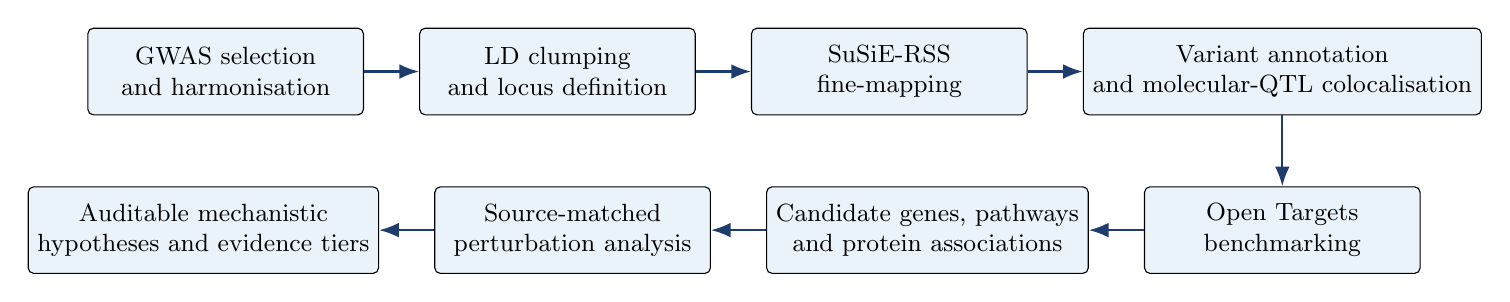
\begin{tikzpicture}[
stage/.style={draw,rounded corners=2pt,fill=lightblue,align=center,minimum width=3.5cm,minimum height=1.1cm,font=\small},
arrow/.style={-{Latex[length=2.5mm]},thick,darkblue}
]
\node[stage] (gwas) {GWAS selection\\and harmonisation};
\node[stage,right=0.7cm of gwas] (loci) {LD clumping\\and locus definition};
\node[stage,right=0.7cm of loci] (fine) {SuSiE-RSS\\fine-mapping};
\node[stage,right=0.7cm of fine] (annot) {Variant annotation\\and molecular-QTL colocalisation};
\node[stage,below=0.9cm of annot] (benchmark) {Open Targets\\benchmarking};
\node[stage,left=0.7cm of benchmark] (systems) {Candidate genes, pathways\\and protein associations};
\node[stage,left=0.7cm of systems] (perturb) {Source-matched\\perturbation analysis};
\node[stage,left=0.7cm of perturb] (mechanism) {Auditable mechanistic\\hypotheses and evidence tiers};
\draw[arrow] (gwas)--(loci);
\draw[arrow] (loci)--(fine);
\draw[arrow] (fine)--(annot);
\draw[arrow] (annot)--(benchmark);
\draw[arrow] (benchmark)--(systems);
\draw[arrow] (systems)--(perturb);
\draw[arrow] (perturb)--(mechanism);
\end{tikzpicture}%
}
\caption{Overview of the GWAS2Mech study design. Each stage retained source identifiers and quality-control fields so that downstream biological hypotheses could be traced to the supporting genetic, molecular, and experimental observations. LD, linkage disequilibrium; QTL, quantitative trait locus.}
\label{fig:study_workflow}
\end{figure}

\subsection{Genetic association processing and fine-mapping}

Seventeen harmonised GWAS datasets were obtained from the GWAS Catalog. Variant identifiers, genome coordinates, alleles, association statistics, sample size, and phenotype metadata were standardised and checked before analysis. A GRCh38 European reference panel derived from the 1000 Genomes 30$\times$ resource supplied allele-frequency and linkage disequilibrium estimates. Genome-wide association signals were clumped into loci, harmonised with the reference panel, and analysed with SuSiE-RSS. The workflow reported posterior inclusion probabilities, nominal 95\% credible sets, convergence diagnostics, and unresolved loci.

\subsection{Functional annotation and molecular-QTL integration}

Fine-mapped variants were annotated with GRCh38-compatible functional resources, including predicted consequences, regulatory annotations, conservation, population frequency, gene constraint, and clinical records. Molecular-QTL analyses then evaluated bulk-tissue, cell-type-specific, and external datasets. Colocalisation support was interpreted as compatibility with a shared statistical signal under the specified model; it was not treated as proof that a named gene was the sole causal effector or that the molecular effect mediated disease risk.

\subsection{External benchmarking and systems-level analyses}

GWAS2Mech loci, credible sets, genes, and molecular evidence were compared with the Open Targets Genetics release recorded in the resource audit. Candidate genes passing the study's quality-control rules were analysed for pathway over-representation and leave-one-gene-out or leave-one-region-out sensitivity. STRING and BioGRID supplied complementary protein-association context \cite{Szklarczyk2025STRING,Oughtred2021BioGRID}. Network enrichment, direct physical edges, and database-added connector proteins were reported separately to prevent network expansion from being mistaken for additional genetic support.

\subsection{Perturbation analysis and evidence integration}

Public single-cell perturbation datasets were screened for usable contrasts involving prioritised genes. Within each annotated gene--dataset contrast, target-perturbed cells were compared with the identified control population, and source-matched pathway gene sets were tested by gene-set enrichment analysis \cite{Subramanian2005GSEA,Peidli2024scPerturb}. The final integration retained representative GWAS and QTL variants, colocalisation posterior, pathway-driver status, protein-association evidence, normalised enrichment score, experimental model, and missing validation fields. A transcriptional response was not considered a validated disease mechanism unless the genetic gene assignment, molecular direction, target perturbation, and downstream pathway response could be aligned.

\subsection{Statistical interpretation and reporting}

Thresholds, denominators, and quality-control exclusions were recorded for every analytical stage. Counts of loci, credible sets, genes, pathways, and experimental records represent different units and were not combined as independent discoveries. False-discovery-rate-adjusted pathway statistics and perturbation statistics arose from separate tests. The detailed subsections below state the relevant implementation choices before each result to preserve a complete computational audit. Workflow identifiers follow the executable pipeline; setup, validation, and plotting stages do not receive separate biological-results subsections.

\section{Results}
\label{sec:results}

\subsection{GWAS dataset selection and acquisition (workflow steps 1--2)}
\label{sec:gwas_download}

\subsubsection{Identification and selection of GWAS datasets}

Genome-wide association study (GWAS) summary statistics
were retrieved from the GWAS Catalog for Parkinson's
disease and related phenotypes in populations of
European ancestry. The datasets included direct
Parkinson's disease case--control associations,
family-history-based proxy phenotypes, medication-use
phenotypes, Parkinson's disease motor subtypes, and
levodopa-induced dyskinesia.

Each GWAS dataset was identified using its unique GWAS
Catalog study accession (GCST). Associated publication
metadata, phenotype descriptions, ancestry, genome
assembly, participant numbers, case--control composition,
and available effect estimates were collected to
characterise the input studies.

A total of 17 GWAS datasets were downloaded. The datasets
were obtained as harmonised summary-statistic files,
providing variant-level association statistics rather
than individual-level participant genotypes.

The downloaded data represented several distinct
phenotype definitions. In particular, family-history
associations and medication-use phenotypes were retained
as related but non-equivalent measures of Parkinson's
disease. Similarly, motor-subtype and treatment-response
studies were considered separately from disease-risk
GWAS datasets.

Table~\ref{tab:gwas_studies} summarises the study
characteristics and sample sizes.

\begingroup
\scriptsize
\setlength{\tabcolsep}{3pt}

\begin{longtable}{@{}p{2.15cm}p{2.75cm}p{4.15cm}p{2.15cm}p{2.8cm}@{}}
\caption{Characteristics of the 17 European-ancestry
GWAS datasets retrieved for Parkinson's disease
and related phenotypes.}
\label{tab:gwas_studies}\\

\toprule
\textbf{GCST accession} &
\textbf{Study} &
\textbf{Phenotype} &
\textbf{Total N} &
\textbf{Cases / Controls} \\
\midrule
\endfirsthead

\multicolumn{5}{l}{
\textit{Table~\thetable\ continued from previous page}
}\\
\toprule
\textbf{GCST accession} &
\textbf{Study} &
\textbf{Phenotype} &
\textbf{Total N} &
\textbf{Cases / Controls} \\
\midrule
\endhead

\midrule
\multicolumn{5}{r}{\textit{Continued on next page}}\\
\endfoot

\bottomrule
\endlastfoot

GCST90104087 &
Le Guen (2021) &
Parkinson's disease, chromosome X &
564,139 & 16,521 / 547,618 \\

GCST90475830 &
Verma (2024) &
Parkinson's disease &
448,956 & 8,704 / 440,252 \\

GCST90476961 &
Verma (2024) &
Parkinson's disease &
315,668 & 4,047 / 311,621 \\

GCST90104085 &
Le Guen (2021) &
Parkinson's disease, chromosome X &
302,908 & 5,328 / 297,580 \\

GCST90104086 &
Le Guen (2021) &
Parkinson's disease, chromosome X &
261,231 & 10,002 / 251,229 \\

GCST90319903 &
Doostparast Torshizi (2024) &
Parkinson's disease &
161,740 & 2,864 / 158,876 \\

GCST90473307 &
UK Biobank WGS Consortium (2025) &
ICD-10 G20: Parkinson's disease &
458,440 & 4,217 / 454,223 \\

GCST90043734 &
Jiang (2021) &
Parkinson's disease, PheCode 332 &
456,348 & 294 / 456,054 \\

GCST90042681 &
Jiang (2021) &
Maternal history of Parkinson's disease &
416,553 & 6,877 / 409,676 \\

GCST90435905 &
Zhou (2018) &
Parkinson's disease, PheCode 332 &
396,336 & 1,127 / 395,209 \\

GCST90042668 &
Jiang (2021) &
Paternal history of Parkinson's disease &
393,679 & 9,960 / 383,719 \\

GCST90079817 &
Backman (2021) &
ICD-10 G20: Parkinson's disease &
387,664 & 1,827 / 385,837 \\

GCST90042694 &
Jiang (2021) &
Sibling history of Parkinson's disease &
355,975 & 1,976 / 353,999 \\

GCST90476962 &
Verma (2024) &
Medication use for Parkinson's disease &
315,668 & 3,573 / 312,095 \\

GCST90281037 &
Sosero (2024) &
Levodopa-induced dyskinesia &
4,787 & 1,612 / 3,175 \\

GCST90000015 &
Alfradique-Dunham (2021) &
Parkinson's motor-subtype quantitative score &
3,212 & -- \\

GCST90000014 &
Alfradique-Dunham (2021) &
Parkinson's motor-subtype comparison &
2,829 & -- \\

\end{longtable}
\endgroup

For quantitative and within-case motor-subtype
analyses, conventional disease-case and population-control
counts were not applicable or were not fully specified
in the extracted metadata. These quantities are therefore
not reported as conventional case--control samples.

Importantly, the datasets were not assumed to be
statistically independent. Several studies used UK
Biobank or Million Veteran Program data, and some
datasets evaluated related phenotypes within potentially
overlapping cohorts.

\subsubsection{Downloaded GWAS variant records}

The 17 downloaded datasets collectively contained
269,271,867 variant-association records before quality
control. This number represents the sum of records across
individual GWAS files and does not represent an equal
number of unique genomic variants.

The number of association records differed substantially
between studies because of differences in genotyping,
imputation, sequencing technologies, variant coverage,
and study design.

For example, the UK Biobank whole-genome sequencing
GWAS (GCST90473307) contained 84,399,074 initial
variant records, whereas each chromosome-X dataset
from Le Guen and colleagues contained 209,339 records.

These study-specific differences were retained in the
downstream data inventory rather than combining all
summary statistics into a single meta-analysis.


\subsection{GWAS harmonisation and quality control (workflow step 2)}
\label{sec:gwas_qc}

\subsubsection{Harmonisation and quality-control procedures}

Quality control was applied independently to each GWAS
dataset using GWASLab within the GWAS2Mech processing
pipeline.

The objective was to produce consistently formatted
variant-association statistics suitable for subsequent
reference-panel matching, linkage disequilibrium
clumping, and fine-mapping.

The processing procedure included standardisation of
chromosome identifiers, genomic positions and allele
representations, examination of association statistics,
normalisation of supported allele representations,
identification of duplicate records, and exclusion of
invalid or unsuitable entries.

The quality-control pipeline employed the GWASLab
\texttt{basic\_check} procedure with variant removal,
duplicate removal, and allele normalisation enabled.

Variants were subsequently required to have nonmissing
P-values within the interval $[0,1]$. Association
statistics were reorganised into a consistent set of
columns, including chromosome, position, variant
identifier, effect allele, other allele, effect size,
standard error, P-value, effect-allele frequency,
minor-allele frequency, sample size, imputation
information when available, and Z-score.

For binary traits, odds ratios were represented on the
log-odds scale where required. Where possible,
standardised Z-scores were obtained from the reported
effect size and standard error or reconstructed using
the available association statistics.

Missing variant-level sample sizes were supplemented
using the study-level total sample size when available,
with their provenance retained.

Table~\ref{tab:gwas_qc_parameters} describes the
implemented quality-control procedures.

\begin{table}[htbp]
\centering
\small
\caption{Quality-control operations applied to GWAS
summary statistics.}
\label{tab:gwas_qc_parameters}

\begin{tabularx}{\linewidth}{@{}p{0.28\linewidth}X@{}}
\toprule
\textbf{Operation} & \textbf{Implementation} \\
\midrule

Input genome assembly &
Harmonised GRCh38 genomic coordinates. \\

Chromosome and position checks &
Invalid or missing chromosome and genomic position
information assessed using GWASLab. \\

Allele checks &
Effect and other alleles standardised; supported
allele representations normalised. \\

Association-statistic checks &
GWASLab sanity checks applied to available P-values,
effect sizes, standard errors, Z-scores, sample sizes,
odds ratios, and related statistical fields. \\

Duplicate handling &
Duplicate SNP identifiers, rsIDs, variant-coordinate
records, and multiallelic representations examined.
The pipeline retained the best-supported record
according to its duplicate-resolution procedure. \\

P-value validity &
Missing P-values excluded; remaining values required
to satisfy $0 \leq P \leq 1$. \\

Allele frequency and INFO &
Available frequency and imputation-information fields
retained and assessed; no additional user-specified
global MAF or INFO threshold was imposed at this step. \\

Sample-size handling &
Variant-level sample size retained when available;
missing values supplemented from study-level
\texttt{N\_TOTAL} where supported. \\

GWAS significance threshold &
$P < 5 \times 10^{-8}$. \\

Standardised output &
\texttt{CHR, POS, SNP, EA, NEA, BETA, SE, P, EAF,
MAF, N, INFO, Z}. \\

\bottomrule
\end{tabularx}
\end{table}

\subsubsection{Variant retention following quality control}

Across the 17 datasets, 266,128,410 of the
269,271,867 initial variant records were retained
following quality control, corresponding to a
retention rate of approximately 98.83\%.

A total of 3,143,457 records were removed
(approximately 1.17\%).

The largest absolute number of removed records
occurred in the whole-genome sequencing dataset
GCST90473307, which retained 81,595,123 of its
84,399,074 initial records.

The quality-controlled datasets contained a combined
total of 13,148 genome-wide significant
variant-association records across the 17 studies.

Table~\ref{tab:gwas_qc_results} presents the
study-specific retention and significance counts.

\begingroup
\scriptsize
\setlength{\tabcolsep}{4pt}

\begin{longtable}{@{}lrrrr@{}}
\caption{Number of GWAS variant-association records
before and after quality control. Genome-wide
significance was defined as $P < 5 \times 10^{-8}$.}
\label{tab:gwas_qc_results}\\

\toprule
\textbf{GWAS accession} &
\textbf{Before QC} &
\textbf{After QC} &
\textbf{Removed} &
\textbf{Significant} \\
\midrule
\endfirsthead

\multicolumn{5}{l}{\textit{Continued from previous page}}\\
\toprule
\textbf{GWAS accession} &
\textbf{Before QC} &
\textbf{After QC} &
\textbf{Removed} &
\textbf{Significant} \\
\midrule
\endhead

\midrule
\multicolumn{5}{r}{\textit{Continued on next page}}\\
\endfoot
\bottomrule
\endlastfoot

GCST90104087 & 209,339 & 209,339 & 0 & 32 \\
GCST90475830 & 19,670,763 & 19,603,221 & 67,542 & 3,642 \\
GCST90476961 & 19,607,622 & 19,540,506 & 67,116 & 23 \\
GCST90104085 & 209,339 & 209,339 & 0 & 32 \\
GCST90104086 & 209,339 & 209,339 & 0 & 32 \\
GCST90319903 & 16,692,835 & 16,668,207 & 24,628 & 3,167 \\
GCST90473307 & 84,399,074 & 81,595,123 & 2,803,951 & 3,246 \\
GCST90043734 & 11,831,294 & 11,831,292 & 2 & 0 \\
GCST90042681 & 11,831,277 & 11,831,275 & 2 & 2,966 \\
GCST90435905 & 27,940,507 & 27,834,350 & 106,157 & 0 \\
GCST90042668 & 11,831,457 & 11,831,455 & 2 & 1 \\
GCST90079817 & 393,573 & 386,728 & 6,845 & 0 \\
GCST90042694 & 11,831,226 & 11,831,224 & 2 & 0 \\
GCST90476962 & 19,607,622 & 19,540,506 & 67,116 & 2 \\
GCST90281037 & 5,561,604 & 5,561,527 & 77 & 0 \\
GCST90000015 & 14,580,738 & 14,580,728 & 10 & 5 \\
GCST90000014 & 12,864,258 & 12,864,251 & 7 & 0 \\

\midrule
\textbf{Total} &
\textbf{269,271,867} &
\textbf{266,128,410} &
\textbf{3,143,457} &
\textbf{13,148} \\

\end{longtable}
\endgroup

All 17 datasets were marked as successfully processed
by the GWAS2Mech quality-control procedure. However,
successful file-level quality control does not imply
equivalent statistical power or phenotype validity.

For example, several studies had relatively small
numbers of Parkinson's disease cases, and some
datasets exhibited unusually low genomic inflation
statistics. Such characteristics may influence the
number and reliability of detectable associations.

Additionally, three chromosome-X GWAS accessions
(GCST90104085, GCST90104086 and GCST90104087)
produced identical quality-control association
summaries despite having different reported sample
sizes. These records were flagged for verification
of their source files and should not be interpreted
as independent genetic replications without
further investigation.


\subsection{European linkage disequilibrium reference panel (workflow step 4)}
\label{sec:reference_panel}

\subsubsection{Reference-panel selection}

To characterise linkage disequilibrium (LD) between
genetic variants, we prepared an ancestry-matched
reference panel from the high-coverage 1000 Genomes
Project sequencing resource.

The 1000 Genomes 30$\times$ resource was selected
because it provides phased genetic variants in
GRCh38 coordinates, including single-nucleotide
variants and insertion/deletion variants, together
with structural-variant records represented in the
source panel.

The original high-coverage resource comprised
3,202 sequenced individuals. The pipeline used the
designated unrelated subset of 2,504 individuals
as the starting population resource, from which
European-ancestry individuals were selected.

The final European panel contained 503 individuals
drawn from five 1000 Genomes populations:

\begin{itemize}
    \item CEU: 99 individuals
    \item FIN: 99 individuals
    \item GBR: 91 individuals
    \item IBS: 107 individuals
    \item TSI: 107 individuals
\end{itemize}

The final panel was constructed separately for the
22 autosomal chromosomes and stored in PLINK 2
genotype-reference format.

The panel contained 70,692,015 variant records
across chromosomes 1--22.

\begin{table}[htbp]
\centering
\small
\caption{Characteristics of the prepared European
1000 Genomes 30$\times$ LD reference panel.}
\label{tab:reference_panel}

\begin{tabularx}{\linewidth}{@{}p{0.43\linewidth}X@{}}
\toprule
\textbf{Characteristic} & \textbf{Value} \\
\midrule

Reference resource &
1000 Genomes high-coverage, 30$\times$ sequencing \\

Reference release &
NYGC high-coverage 1000 Genomes resource (2022) \\

Genome assembly &
GRCh38 \\

Individuals in source sequencing resource &
3,202 \\

Designated unrelated individuals in global resource &
2,504 \\

Selected ancestry &
European (EUR) \\

European individuals retained &
503 \\

CEU / FIN / GBR &
99 / 99 / 91 \\

IBS / TSI &
107 / 107 \\

Chromosomes included &
Autosomes 1--22 \\

Completed chromosome panels &
22 / 22 \\

Variants in final EUR panel &
70,692,015 \\

Genotype representation &
Phased source VCF converted to PLINK 2 PGEN format \\

Variant-identity handling &
Reference allele, alternate allele, chromosome
and position retained for downstream harmonisation;
duplicate identifiers resolved during preparation. \\

\bottomrule
\end{tabularx}
\end{table}

\subsubsection{Reference-panel processing}

Ancestry-specific samples were selected from the
source phased variant-call files. Genotype information
for the selected European samples was extracted on
a chromosome-by-chromosome basis and converted to
PLINK 2 reference files.

The pipeline preserved the reference allele and
alternate allele representations from the GRCh38
source data. Variant identifiers were retained
where available, with coordinate- and allele-based
identifiers generated for variants lacking an
appropriate identifier.

Duplicate identifiers were checked during reference
construction, with inconsistent duplicated entries
excluded according to the reference-panel processing
configuration.

All 22 autosomal reference panels completed
successfully without reported chromosome-level
failures.

The final number of variants varied between
chromosomes. Chromosome 2 contained 6,088,598
variants, chromosome 1 contained 5,759,060, and
chromosome 21 contained 1,002,753.

The total of 70,692,015 refers to variants in the
completed European reference panels. A corresponding
total number of variants before European subsetting
and reference processing was not provided in the
current reference statistics and is therefore not
reported as a measured filtering result.

\subsubsection{Purpose of the LD reference panel}

LD represents the non-random correlation between
alleles at different genomic positions.

A GWAS may identify many statistically significant
variants within the same region because correlated
variants can tag the same underlying association.

The European reference panel was therefore used
to estimate pairwise variant correlations for
LD clumping and subsequent fine-mapping.

For two variants $i$ and $j$, their pairwise
LD correlation was represented using:

\begin{equation}
r_{ij}^{2}
=
\left[
\operatorname{Corr}(G_i,G_j)
\right]^2,
\end{equation}

where $G_i$ and $G_j$ denote genotype dosages
for the two variants in the reference population.

The reference panel was used to characterise LD
rather than to estimate associations with
Parkinson's disease directly.

Chromosome-X associations were not included in
this autosomal reference-panel analysis because
the prepared panels covered chromosomes 1--22.


\subsection{Associated-locus definition by linkage disequilibrium clumping (workflow step 5)}
\label{sec:clumping}

\subsubsection{Reference-panel harmonisation}

Following GWAS quality control and reference-panel
preparation, LD clumping was performed independently
for each GWAS dataset using PLINK 2 and the European
1000 Genomes 30$\times$ reference panel.

The first stage involved mapping GWAS variants
to the reference panel.

Variant matching required concordance of chromosome,
genomic position, and allele identity in GRCh38
coordinates.

Variants without a compatible reference-panel
representation were excluded from the LD-clumping
calculation and recorded in a separate audit.

Unmatched variants were classified according
to their mapping failure, including absence
from the reference panel, incompatible alleles,
or ambiguous mapping.

This harmonisation was performed separately for
each GWAS study.

\subsubsection{LD-clumping parameters}

Clumping was performed using genome-wide significant
variants as candidate index variants.

A primary significance threshold of
$P_1 = 5 \times 10^{-8}$ was applied to identify
eligible index variants.

A secondary threshold of $P_2 = 0.01$ was used
for additional variants considered in the
clumping procedure.

Pairwise LD was estimated using the ancestry-matched
European reference panel. The clumping threshold
was set to $r^2 = 0.1$, with a distance window
of 1,000 kilobases.

For each index variant, nearby variants satisfying
the secondary P-value threshold and the LD
criterion were grouped within the corresponding
clump.

The resulting index variants represented
approximately LD-independent association signals
under the specified clumping parameters.

Clumping did not establish causal variants;
rather, it reduced correlated association
records to representative lead variants.

Table~\ref{tab:clumping_parameters} provides the
parameters used for this analysis.

\begin{table}[htbp]
\centering
\small
\caption{Parameters used for GWAS variant matching
and PLINK 2 LD clumping.}
\label{tab:clumping_parameters}

\begin{tabularx}{\linewidth}{@{}p{0.36\linewidth}X@{}}
\toprule
\textbf{Parameter} & \textbf{Setting} \\
\midrule

Clumping software &
PLINK 2 \\

GWAS genome assembly &
GRCh38 \\

Reference panel &
1000 Genomes 30$\times$ \\

Reference ancestry &
European (EUR) \\

Reference sample size &
503 individuals \\

Chromosomes &
1--22 \\

Variant mapping &
Chromosome, position and allele concordance \\

Primary P-value threshold ($P_1$) &
$5 \times 10^{-8}$ \\

Secondary P-value threshold ($P_2$) &
$0.01$ \\

LD threshold &
$r^2 = 0.1$ \\

Clumping window &
1,000 kb \\

Locus-consolidation procedure &
Overlapping lead-centred $\pm 1$ Mb regions
merged into study-specific loci \\

Candidate-processing chunk size &
500,000 records \\

Unmatched significant variants &
Retained in separate mapping-audit outputs \\

\bottomrule
\end{tabularx}
\end{table}

\subsubsection{Identification of genomic loci}

Following LD clumping, the retained lead variants
were used to define broader genomic loci.

Genomic intervals extending 1 Mb upstream and
downstream of lead variants were constructed
and overlapping intervals were consolidated.

Consequently, a single genomic locus could
contain multiple approximately LD-independent
lead variants.

A locus was therefore distinguished from an
individual lead variant:

\begin{itemize}
    \item A lead variant represented an association
    selected after LD clumping.
    \item A genomic locus represented a broader
    region containing one or more lead variants.
\end{itemize}

This distinction is important for subsequent
fine-mapping, which evaluates candidate causal
variants within genomic regions rather than
assuming that the clumping lead is causal.

\subsubsection{GWAS-specific clumping results}

Across the 17 GWAS datasets, the QC summaries
identified 13,148 genome-wide significant
variant records.

Of these, 96 were reported in the three
chromosome-X studies and were outside the
autosomal reference-panel scope.

Among the remaining 13,052 significant
autosomal records, 12,674 could be matched
to the European 1000 Genomes 30$\times$
reference panel.

The clumping procedure identified a total of
59 lead variants across eight GWAS datasets
with at least one retained autosomal association.

These lead variants were consolidated into
31 study-specific genomic loci.

Table~\ref{tab:gwas_clumping_results} summarises
the results for each GWAS dataset.

\begingroup
\scriptsize
\setlength{\tabcolsep}{3pt}

\begin{longtable}{@{}lrrrrp{5.6cm}@{}}
\caption{LD-clumping results for each GWAS study.
Representative lead positions are shown for studies
with retained signals. Positions are in GRCh38
megabases (Mb), rounded to three decimal places.
They are not complete locus boundaries or a
complete list of all 59 lead variants.}
\label{tab:gwas_clumping_results}\\

\toprule
\textbf{GCST} &
\textbf{GWS} &
\textbf{Matched} &
\textbf{Leads} &
\textbf{Loci} &
\textbf{Representative lead positions} \\
\midrule
\endfirsthead

\multicolumn{6}{l}{
\textit{Continued from previous page}
}\\
\toprule
\textbf{GCST} &
\textbf{GWS} &
\textbf{Matched} &
\textbf{Leads} &
\textbf{Loci} &
\textbf{Representative lead positions} \\
\midrule
\endhead

\midrule
\multicolumn{6}{r}{\textit{Continued on next page}}\\
\endfoot
\bottomrule
\endlastfoot

GCST90000014 &
0 & 0 & 0 & 0 &
-- \\

GCST90000015 &
5 & 4 & 4 & 4 &
chr6:36.725;
chr15:58.516;
chr18:51.140, 75.103 \\

GCST90042668 &
1 & 1 & 1 & 1 &
chr17:42.146 \\

GCST90042681 &
2,966 & 2,900 & 6 & 2 &
chr17:45.771, 45.904, 46.072, 46.106, 46.785 \\

GCST90042694 &
0 & 0 & 0 & 0 &
-- \\

GCST90043734 &
0 & 0 & 0 & 0 &
-- \\

GCST90079817 &
0 & 0 & 0 & 0 &
-- \\

GCST90104085 &
32 & 0 & 0 & 0 &
Chromosome X only; outside autosomal panel \\

GCST90104086 &
32 & 0 & 0 & 0 &
Chromosome X only; outside autosomal panel \\

GCST90104087 &
32 & 0 & 0 & 0 &
Chromosome X only; outside autosomal panel \\

GCST90281037 &
0 & 0 & 0 & 0 &
-- \\

GCST90319903 &
3,167 & 3,101 & 14 & 7 &
chr2:168.287;
chr4:89.716;
chr17:45.760, 45.970, 46.072 \\

GCST90435905 &
0 & 0 & 0 & 0 &
-- \\

GCST90473307 &
3,246 & 3,149 & 13 & 7 &
chr2:168.310;
chr4:89.716, 89.853;
chr17:45.825, 45.970 \\

GCST90475830 &
3,642 & 3,495 & 13 & 4 &
chr4:89.705;
chr17:45.679, 45.904, 46.053, 46.106 \\

GCST90476961 &
23 & 22 & 6 & 4 &
chr2:61.028, 61.908, 62.073, 168.287;
chr4:89.705 \\

GCST90476962 &
2 & 2 & 2 & 2 &
chr4:89.705;
chr13:36.533 \\

\midrule
\textbf{Total} &
\textbf{13,148} &
\textbf{12,674} &
\textbf{59} &
\textbf{31} &
\textbf{Study-specific counts} \\

\end{longtable}
\endgroup

GWS denotes genome-wide significant variant records.
The matched column reports significant variants
successfully mapped to the autosomal LD reference.
The lead and locus columns represent the respective
study-specific outputs of the clumping pipeline.

The representative coordinates are examples printed
by the Step05 clumping audit. Complete lead-variant
identifiers and locus intervals should be reported
from the corresponding per-study
\texttt{lead\_variants.tsv} and downstream locus
definition files.

\subsubsection{Comparison between GWAS significance
and independent association signals}

The reduction in the number of variant associations
after LD clumping was substantial.

For example, GCST90475830 contained 3,642
genome-wide significant variants, of which
3,495 were successfully matched to the LD
reference panel.

These mapped associations produced 13 lead
variants, subsequently consolidated into
four broader genomic loci.

Similarly, GCST90319903 contained 3,167
significant variants, of which 3,101 matched
the reference panel. These were represented
by 14 lead variants grouped into seven loci.

In the whole-genome sequencing dataset
GCST90473307, 3,149 of 3,246 significant
variants matched the reference, resulting
in 13 lead variants distributed across
seven loci.

The large difference between the number
of significant variants and lead variants
illustrates the contribution of LD to
GWAS association patterns.

However, the 59 identified leads should
not be interpreted as 59 independent
biological discoveries. Their independence
was defined by the selected LD threshold
and reference panel, and some loci overlap
between different GWAS datasets.

\subsubsection{Unmapped association signals}

Although most genome-wide significant
autosomal variants matched the reference,
a subset could not be mapped because of
missing reference variants, incompatible
alleles, or ambiguous representations.

In most instances, unmatched significant
variants occurred close to retained
lead variants and therefore remained
represented at the regional level.

However, three significant association
regions were flagged as lacking a mapped
lead within the 1 Mb search window:

\begin{itemize}

\item GCST90000015:
chr2:199,727,717, with an association
P-value of approximately $2.4 \times 10^{-8}$.

\item GCST90473307:
chr3:128,656,141, with an association
P-value of approximately $5.7 \times 10^{-9}$.

\item GCST90473307:
chr12:37,686,151, with an association
P-value of approximately $7.1 \times 10^{-9}$.

\end{itemize}

These regions were not represented among
the retained clumping leads because their
significant variants could not be matched
to the available reference panel.

Their absence from the clumping output
does not invalidate the original GWAS
associations. Rather, it identifies a
limitation of reference-panel coverage
that may require further investigation.

\subsubsection{Output for subsequent fine-mapping}

The output of this stage consisted of
study-specific lead-variant tables,
reference-mapped association variants,
genomic locus definitions, and audit
reports describing unmatched significant
variants.

These outputs were used to establish
the genomic regions subsequently
considered for statistical fine-mapping.

Whereas LD clumping identified representative
association signals, fine-mapping was intended
to assign posterior support to candidate
causal variants within those regions.

Thus, the principal outcome of the initial
GWAS processing stages was a harmonised
collection of study-specific genomic
association regions and their supporting
variant-level statistics, rather than a
definitive set of causal genes or variants.

 
% ==============================================================
% GWAS2Mech: STEP 5 -- STATISTICAL FINE-MAPPING
%
% Add to your LaTeX preamble (if not already loaded):
%
% \usepackage{booktabs}
% \usepackage{longtable}
% \usepackage{array}
% \usepackage{amsmath}
% \usepackage{tikz}
% \usetikzlibrary{arrows.meta,positioning,shapes.geometric}
%
% The bibliography keys are provided after this section.
% ==============================================================

\subsection{Statistical fine-mapping of GWAS loci (workflow step 6)}
\label{sec:finemapping}

\subsubsection{Rationale for statistical fine-mapping}

Following linkage disequilibrium (LD) clumping, the
identified genomic regions were subjected to statistical
fine-mapping to prioritise variants potentially responsible
for the observed GWAS associations.

Although LD clumping identifies representative lead
variants, these variants are not necessarily causal.
Several variants in the same genomic region may display
similar association statistics because of correlations
between their alleles.

Fine-mapping therefore seeks to distinguish candidate
causal variants from correlated variants by jointly
modelling GWAS association statistics and local LD
structure.

We employed Sum of Single Effects Regression using
Summary Statistics (SuSiE-RSS), implemented in the
\texttt{susieR} R package \cite{Zou2022,Wang2020}.

SuSiE-RSS permits multiple association signals within
a locus and estimates the posterior inclusion probability
(PIP) of each candidate variant, together with
credible sets representing individual association signals.

\subsubsection{Fine-mapping workflow}

Fine-mapping was performed independently for each
eligible GWAS dataset using the harmonised GRCh38
summary statistics and the European 1000 Genomes
high-coverage (30$\times$) reference panel.

First, genomic loci were reconstructed from the Step 4
lead variants. Each lead variant was extended by
1 Mb upstream and downstream, and overlapping
intervals were merged into study-specific loci.

All available quality-controlled GWAS variants within
each locus were extracted, including variants that did
not individually achieve genome-wide significance.

Variants were subsequently matched to the LD reference
panel by genomic position and allele identity.
Association Z-scores were oriented consistently with
the reference-panel allele coding.

Reference variants were filtered using a minor allele
frequency threshold of 0.01 and a maximum genotype
missingness rate of 0.05. A maximum of 15,000 variants
per locus was imposed for LD matrix construction.

For loci exceeding this limit, a deterministic selection
procedure retained variants surrounding the independent
lead positions. Such downsampling was recorded and
flagged during quality assessment.

Signed pairwise LD correlations were calculated using
PLINK 2 and supplied to SuSiE-RSS together with the
harmonised GWAS Z-scores and study-specific sample size.

For binary traits, effective sample size was used where
available:

\begin{equation}
N_{\mathrm{eff}} =
\frac{4N_{\mathrm{cases}}N_{\mathrm{controls}}}
{N_{\mathrm{cases}}+N_{\mathrm{controls}}}.
\end{equation}

For continuous traits, the total sample size was used.

SuSiE-RSS was executed using a target credible-set
coverage of 95\%, with an initial allowance of ten
single-effect components, increased according to the
number of clumped leads where necessary, up to
a maximum of twenty components.

Residual variance estimation was disabled because
the LD matrices were obtained from an external
reference panel.

The posterior inclusion probability for variant $j$
can be expressed conceptually as

\begin{equation}
\mathrm{PIP}_{j}
=
\Pr\left(
\beta_j \neq 0
\mid
\mathbf{z},\mathbf{R},N
\right),
\end{equation}

where $\mathbf{z}$ denotes the vector of GWAS
association Z-scores, $\mathbf{R}$ represents the
signed LD correlation matrix, and $N$ denotes the
effective or total GWAS sample size, as appropriate.

For each inferred effect, SuSiE-RSS was used to construct
a credible set with a nominal posterior coverage
of 95\%.

Model convergence, LD consistency, possible allele
orientation errors, credible-set purity, and retention
of the original clumping leads were examined as
quality-control criteria.

% --------------------------------------------------------------
% Figure: Fine-mapping workflow with real study example
% --------------------------------------------------------------

\begin{figure}[htbp]
\centering

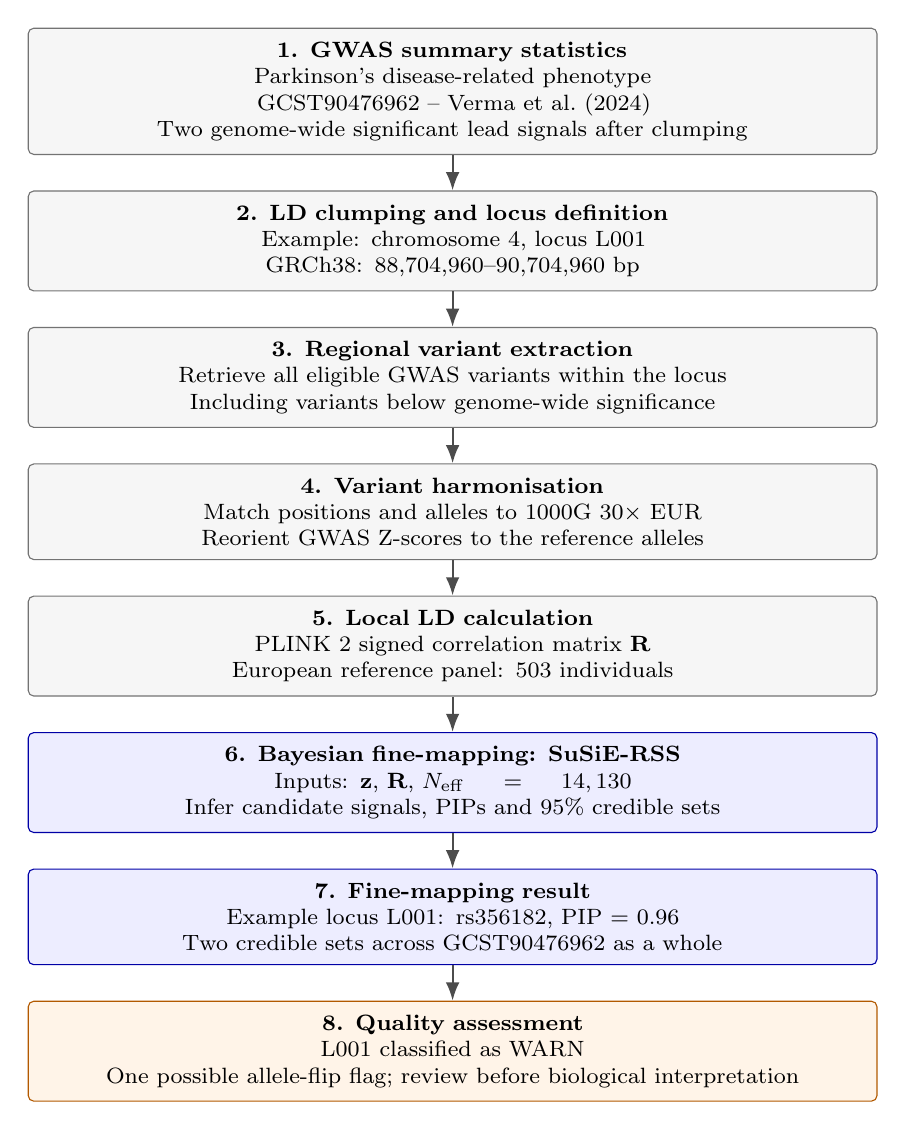
\begin{tikzpicture}[
    node distance=4.5mm,
    >=Latex,
    base/.style={
        rectangle,
        rounded corners=2pt,
        draw=black!55,
        fill=gray!7,
        text width=0.86\linewidth,
        align=center,
        inner sep=5pt,
        font=\footnotesize
    },
    emphasis/.style={
        base,
        fill=blue!7,
        draw=blue!65!black
    },
    caution/.style={
        base,
        fill=orange!9,
        draw=orange!70!black
    },
    arrow/.style={
        ->,
        thick,
        draw=black!70
    }
]

\node[base] (gwas) {
    \textbf{1. GWAS summary statistics}\\
    Parkinson's disease-related phenotype\\
    GCST90476962 -- Verma et al.\ (2024)\\
    Two genome-wide significant lead signals after clumping
};

\node[base, below=of gwas] (locus) {
    \textbf{2. LD clumping and locus definition}\\
    Example: chromosome 4, locus L001\\
    GRCh38: 88,704,960--90,704,960 bp
};

\node[base, below=of locus] (extract) {
    \textbf{3. Regional variant extraction}\\
    Retrieve all eligible GWAS variants within the locus\\
    Including variants below genome-wide significance
};

\node[base, below=of extract] (harmonise) {
    \textbf{4. Variant harmonisation}\\
    Match positions and alleles to 1000G 30$\times$ EUR\\
    Reorient GWAS Z-scores to the reference alleles
};

\node[base, below=of harmonise] (ld) {
    \textbf{5. Local LD calculation}\\
    PLINK 2 signed correlation matrix $\mathbf{R}$\\
    European reference panel: 503 individuals
};

\node[emphasis, below=of ld] (susie) {
    \textbf{6. Bayesian fine-mapping: SuSiE-RSS}\\
    Inputs: $\mathbf{z}$, $\mathbf{R}$, $N_{\mathrm{eff}}=14,130$\\
    Infer candidate signals, PIPs and 95\% credible sets
};

\node[emphasis, below=of susie] (result) {
    \textbf{7. Fine-mapping result}\\
    Example locus L001: rs356182, PIP = 0.96\\
    Two credible sets across GCST90476962 as a whole
};

\node[caution, below=of result] (qc) {
    \textbf{8. Quality assessment}\\
    L001 classified as WARN\\
    One possible allele-flip flag; review before
    biological interpretation
};

\draw[arrow] (gwas) -- (locus);
\draw[arrow] (locus) -- (extract);
\draw[arrow] (extract) -- (harmonise);
\draw[arrow] (harmonise) -- (ld);
\draw[arrow] (ld) -- (susie);
\draw[arrow] (susie) -- (result);
\draw[arrow] (result) -- (qc);

\end{tikzpicture}

\caption{
GWAS2Mech statistical fine-mapping workflow illustrated
using the observed results for GCST90476962
(Verma et al., 2024).
The original association region on chromosome 4
was analysed using SuSiE-RSS with European reference LD.
The variant rs356182 achieved a posterior inclusion
probability of approximately 0.96.
The reported credible-set count refers to the entire
GWAS dataset, not exclusively to the illustrated locus.
A QC warning indicates that the locus requires further
assessment before causal interpretation.
}

\label{fig:finemapping_workflow}
\end{figure}


\subsubsection{GWAS-specific fine-mapping results}

Across the 17 original GWAS datasets, eight contained
autosomal association loci eligible for fine-mapping.

The 59 lead variants identified by LD clumping were
represented by 32 study-specific genomic loci in
the current fine-mapping run. The preceding clumping
audit recorded 31 study-specific loci. In particular,
GCST90473307 had seven loci in the clumping summary
but eight in the fine-mapping inventory. The precise
origin of the extra reconstructed interval has not
been reconciled against the source locus-definition
files; these are stage-specific observed counts and
must not be portrayed as a single internally identical
set of intervals.

All 32 loci completed SuSiE-RSS processing without
a recorded locus-level execution failure.

Fine-mapping identified a total of 69 study-specific
95\% credible sets.

Across the fine-mapped study records, 60 variants
had PIP greater than 0.5, of which 52 had PIP
greater than 0.9.

These totals represent study-specific variant records
and credible sets rather than unique variants or
independent biological signals across all studies.

Table~\ref{tab:finemapping_studies} summarises
the study-specific results.

% --------------------------------------------------------------
% TABLE 1: GWAS publications and fine-mapping results
% --------------------------------------------------------------

\begin{table}[htbp]
\centering
\scriptsize
\setlength{\tabcolsep}{3.5pt}

\caption{
Statistical fine-mapping results across eight
Parkinson's disease and related GWAS datasets.
GWAS accession labels are the primary provenance;
original-publication attributions for all accession
rows should be checked against the Catalog metadata
before external submission.
Leads denote variants retained after LD clumping;
loci denote study-specific genomic regions;
CS denotes 95\% credible sets.
High-PIP variants are counted within each GWAS.
QC is reported as PASS/WARN locus counts.
}

\label{tab:finemapping_studies}

\resizebox{\textwidth}{!}{%
\begin{tabular}{@{}llrrrrrrr@{}}

\toprule

\textbf{GWAS accession} &
\textbf{Publication} &
\textbf{Leads} &
\textbf{Loci} &
\textbf{$N$ used} &
\textbf{CS} &
\textbf{PIP $>0.9$} &
\textbf{PASS} &
\textbf{WARN} \\

\midrule

GCST90000015 &
Alfradique-Dunham (2021) \cite{AlfradiqueDunham2021} &
4 & 4 & 3,212 & 0 & 0 & 0 & 4 \\

GCST90042668 &
Jiang (2021) \cite{Cerezo2025} &
1 & 1 & 38,832 & 0 & 0 & 0 & 1 \\

GCST90042681 &
Jiang (2021) \cite{Cerezo2025} &
6 & 2 & 27,054 & 8 & 6 & 0 & 2 \\

GCST90319903 &
Doostparast Torshizi (2024) \cite{Cerezo2025} &
14 & 7 & 11,253 & 19 & 16 & 0 & 7 \\

GCST90473307 &
UKB WGS Consortium (2025) \cite{UKBWGS2025} &
13 & 8 & 16,713 & 15 & 11 & 0 & 8 \\

GCST90475830 &
Verma (2024) \cite{Verma2024} &
13 & 4 & 34,141 & 14 & 11 & 1 & 3 \\

GCST90476961 &
Verma (2024) \cite{Verma2024} &
6 & 4 & 15,980 & 11 & 7 & 1 & 3 \\

GCST90476962 &
Verma (2024) \cite{Verma2024} &
2 & 2 & 14,130 & 2 & 1 & 0 & 2 \\

\midrule

\textbf{Total} &
-- &
\textbf{59} &
\textbf{32} &
-- &
\textbf{69} &
\textbf{52} &
\textbf{2} &
\textbf{30} \\

\bottomrule
\end{tabular}%
}

\end{table}

The sample sizes shown in Table~\ref{tab:finemapping_studies}
are the values supplied to SuSiE-RSS, rather than
necessarily the total number of participants in each GWAS.
For binary studies these generally correspond to the
effective sample size, whereas the continuous
motor-subtype study used the total sample size.

The number of credible sets varied substantially
between studies.

GCST90319903 produced 19 credible sets across seven
fine-mapped loci, while GCST90473307 produced
15 credible sets across eight loci.

GCST90475830 yielded 14 credible sets across four loci,
and GCST90476961 yielded 11 credible sets across four loci.

In contrast, GCST90000015 and GCST90042668 produced
no retained credible sets despite completing fine-mapping.

Thus, the existence of a genome-wide significant lead
association did not guarantee the identification of
a sufficiently resolved credible set.


\subsubsection{Genomic distribution of fine-mapped loci}

The current fine-mapping analysis defined 32
study-specific regions across the eight eligible GWAS
datasets.

Table~\ref{tab:finemapping_regions} reports the locus
identifiers, genomic intervals and fine-mapping
quality-control classifications.

Coordinates are reported in GRCh38 base pairs.
Because fine-mapping was performed independently for
each GWAS dataset, overlapping intervals in different
studies were retained as separate study-specific loci.

% --------------------------------------------------------------
% TABLE 2: Individual fine-mapped genomic regions
% --------------------------------------------------------------

\begingroup
\scriptsize
\setlength{\tabcolsep}{5pt}
\renewcommand{\arraystretch}{1.12}

\begin{longtable}{@{}llp{7.0cm}l@{}}

\caption{
Genomic intervals of the 32 study-specific loci
processed using SuSiE-RSS; the upstream clumping audit
reported 31 loci (one additional interval in
GCST90473307 at this stage remains to be reconciled).
Coordinates are based on GRCh38.
The two intervals absent from the supplied summary log
require extraction from their loci definition files.
}
\label{tab:finemapping_regions}\\

\toprule
\textbf{GWAS accession} &
\textbf{Locus} &
\textbf{Genomic region (GRCh38, bp)} &
\textbf{QC} \\
\midrule
\endfirsthead

\multicolumn{4}{l}{
\textit{Table continued from previous page}
}\\
\toprule
\textbf{GWAS accession} &
\textbf{Locus} &
\textbf{Genomic region (GRCh38, bp)} &
\textbf{QC} \\
\midrule
\endhead

\midrule
\multicolumn{4}{r}{\textit{Continued on next page}}\\
\endfoot

\bottomrule
\endlastfoot

GCST90000015 & L001 &
chr6:35,725,362--37,725,362 & WARN \\
GCST90000015 & L002 &
chr15:57,515,688--59,515,688 & WARN \\
GCST90000015 & L003 &
chr18:50,139,811--52,139,811 & WARN \\
GCST90000015 & L004 &
chr18:74,103,246--76,103,246 & WARN \\

\midrule

GCST90042668 & L001 &
chr17:41,146,497--43,146,497 & WARN \\

\midrule

GCST90042681 & L001 &
chr12:39,340,400--41,340,400 & WARN \\
GCST90042681 & L002 &
chr17:44,771,384--47,785,247 & WARN \\

\midrule

GCST90319903 & L001 &
chr1:154,236,376--156,236,376 & WARN \\
GCST90319903 & L002 &
chr2:167,286,525--169,286,525 & WARN \\
GCST90319903 & L003 &
chr4:88,716,450--90,821,664 & WARN \\
GCST90319903 & L004 &
chr12:39,340,400--41,340,400 & WARN \\
GCST90319903 & L005 &
chr14:53,881,109--55,881,109 & WARN \\
GCST90319903 & L006 &
chr17:44,759,587--47,785,767 & WARN \\
GCST90319903 & L007 &
chr19:43,908,684--45,908,684 & WARN \\

\midrule

GCST90473307 & L001 &
chr1:154,236,376--156,236,376 & WARN \\
GCST90473307 & L002 &
chr2:167,309,772--169,309,772 & WARN \\
GCST90473307 & L003 &
chr3:164,216,729--166,216,729 & WARN \\
GCST90473307 & L004 &
chr4:1--1,912,343 & WARN \\
GCST90473307 & L005 &
chr4:88,716,450--90,852,931 & WARN \\
GCST90473307 & L006 &
chr12:39,340,400--41,340,400 & WARN \\
GCST90473307 & L007 &
chr14:53,870,033--55,870,033 & WARN \\
GCST90473307 & L008 &
chr17:44,486,240--46,969,671 & WARN \\

\midrule

GCST90475830 & L001 &
chr2:167,286,525--169,286,525 & WARN \\
GCST90475830 & L002 &
chr4:88,704,947--90,704,947 & PASS \\
GCST90475830 & L003 &
chr12:39,340,400--41,340,400 & WARN \\
GCST90475830 & L004 &
chr17:44,604,405--47,709,947 & WARN \\

\midrule

GCST90476961 & L001 &
chr2:60,028,470--63,072,723 & WARN \\
GCST90476961 & L002 &
chr2:167,286,525--169,286,525 & WARN \\
GCST90476961 & L003 &
chr4:88,704,960--90,704,960 & PASS \\
GCST90476961 & L004 &
chr17:44,625,426--46,625,426 & WARN \\

\midrule

GCST90476962 & L001 &
chr4:88,704,960--90,704,960 & WARN \\
GCST90476962 & L002 &
chr13:35,532,864--37,532,864 & WARN \\

\end{longtable}
\endgroup


\subsubsection{Posterior prioritisation of candidate variants}

Fine-mapping produced study-specific rankings of
candidate variants according to their posterior
inclusion probabilities.

Several variants achieved very high PIPs in the
Parkinson's disease-associated regions.

For example, in GCST90476962, rs356182 was the
highest-ranked reported variant within locus L001
on chromosome 4, achieving a PIP of approximately 0.96.

Within GCST90319903, variants including rs374035281,
rs16940802 and rs71363566 were reported among
the highest-PIP candidates.

Likewise, GCST90475830 and GCST90476961
reported high-PIP variants including rs62058964
and rs66781068.

However, these probabilities are conditional on the
fine-mapping model, variant inclusion, LD reference
and quality of the association statistics.

A high PIP must therefore not be interpreted as
experimental proof of a causal variant.

Furthermore, variant-level support cannot be assumed
to represent independent replication when different
GWAS analyses include overlapping participants.


\subsubsection{Fine-mapping quality and limitations}

Although all 32 loci completed computational processing,
only two satisfied all implemented fine-mapping
quality-control criteria.

The remaining 30 loci were classified as WARN.

Five locus-level SuSiE-RSS fits failed to converge
within the configured maximum of 500 iterations.

Across the study-specific analyses, 33 possible
allele-flip events were flagged by the diagnostic
procedures. These represent potential inconsistencies
rather than confirmed allele-coding errors.

Warnings also included discrepancies between GWAS
association Z-scores and reference-panel LD,
missing original lead variants after reference matching,
and high-PIP variants outside retained credible sets.

For example, GCST90473307 locus L008,
located at chr17:44,486,240--46,969,671,
did not converge within 500 iterations and was
flagged for three possible allele flips and an
original lead position missing from the final
LD variant set.

Similarly, GCST90319903 locus L006,
located at chr17:44,759,587--47,785,767,
did not converge and was flagged for a possible
allele flip and missing clumping lead positions.

These findings demonstrate that numerical completion
of a fine-mapping run does not necessarily imply
reliable resolution of its causal signals.

The posterior probabilities and credible sets should
therefore be interpreted in conjunction with their
locus-specific quality-control results.

In particular, high-confidence causal claims should
not be based solely on PIP thresholds when the
corresponding loci show non-convergence, possible
allele mismatches, or inconsistencies between
summary statistics and reference LD.

\subsubsection{Worked example of statistical fine-mapping at chromosome 4}
\label{subsec:finemap_worked_chr4}

To illustrate the distinction between lead-variant selection and
fine-mapping, we examined the overlapping chromosome 4 regions in
GCST90475830, GCST90476961, and GCST90476962
\cite{Verma2024}. The lead variants reported by GCST90475830
(locus L002, \texttt{4:89704947:G:C}) and GCST90476961
(locus L003, \texttt{4:89704960:G:A}) were located only 13 base pairs
apart in GRCh38 coordinates. These are different positions, not an
identical lead variant. Their lead-centred 2-Mb intervals overlap
extensively. The GCST90476962 L001 interval spanned
chr4:88,704,960--90,704,960 and was analysed separately using its
own GWAS summary statistics.

In each region, all available quality-controlled regional variants,
not only the lead SNP, were matched to the European-ancestry 1000
Genomes 30$\times$ reference panel. An LD correlation matrix $\mathbf R$
was computed for the harmonised variants; the corresponding association
$Z$-scores $\mathbf z$ and study-specific sample size $N$ were supplied
to SuSiE-RSS \cite{Zou2022}. For GCST90476962, the recorded effective
sample size was
\begin{equation}
N_{\mathrm{eff}} =
\frac{4(3,573)(312,095)}{3,573+312,095}
\approx 14,130.
\end{equation}

In the Sum of Single Effects model, a regression effect is represented
as a sum of $L$ single-effect components:
\begin{equation}
\boldsymbol\beta = \sum_{\ell=1}^{L}\boldsymbol\beta_{\ell},
\qquad \|\boldsymbol\beta_{\ell}\|_0 \leq 1.
\end{equation}
Let $\alpha_{\ell j}$ denote the posterior probability that variant
$j$ is selected for component $\ell$. The posterior inclusion
probability (PIP) is then
\begin{equation}
\mathrm{PIP}_{j}=1-\prod_{\ell=1}^{L}(1-\alpha_{\ell j}),
\end{equation}
whereas a nominal 95\% credible set $C_{\ell}$ collects variants whose
component-specific posterior probabilities satisfy
\begin{equation}
\sum_{j\in C_{\ell}}\alpha_{\ell j}\geq 0.95.
\end{equation}
Thus, the output is a posterior prioritisation of variants and
credible sets, rather than a second genome-wide significance test.

\begin{figure}[htbp]
\centering
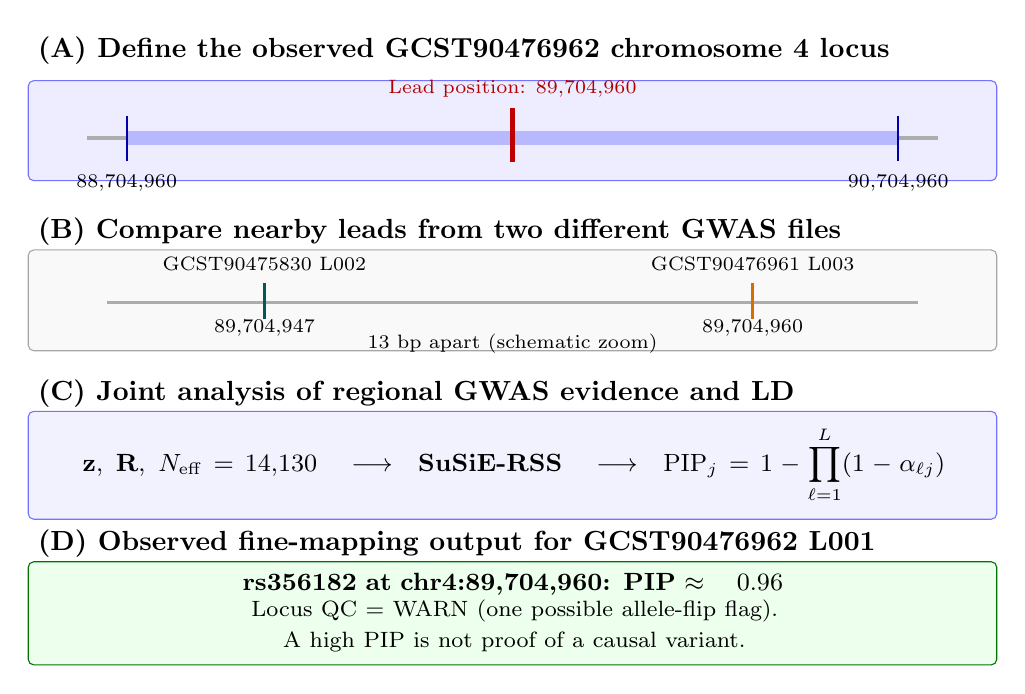
\begin{tikzpicture}[x=1cm,y=1cm,>=Latex,font=\small]
  % Panel A: study-specific physical region
  \node[anchor=west,font=\bfseries] at (0,7.95)
      {(A) Define the observed GCST90476962 chromosome 4 locus};
  \draw[rounded corners=2pt,fill=blue!7,draw=blue!55]
       (0,6.30) rectangle (12.3,7.57);
  \draw[line width=1.4pt,gray!65] (0.75,6.84)--(11.55,6.84);
  \draw[line width=5pt,blue!28] (1.25,6.84)--(11.05,6.84);
  \draw[blue!65!black,thick] (1.25,6.55)--(1.25,7.12);
  \draw[blue!65!black,thick] (11.05,6.55)--(11.05,7.12);
  \draw[red!75!black,line width=1.5pt] (6.15,6.54)--(6.15,7.22);
  \node[font=\scriptsize,anchor=north] at (1.25,6.49) {88,704,960};
  \node[font=\scriptsize,anchor=north] at (11.05,6.49) {90,704,960};
  \node[font=\scriptsize,anchor=south,red!70!black] at (6.15,7.24)
      {Lead position: 89,704,960};
  % Panel B: comparison of real lead coordinates (not to scale)
  \node[anchor=west,font=\bfseries] at (0,5.65)
      {(B) Compare nearby leads from two different GWAS files};
  \draw[rounded corners=2pt,fill=gray!5,draw=black!35]
       (0,4.14) rectangle (12.3,5.42);
  \draw[very thick,gray!65] (1.0,4.75)--(11.3,4.75);
  \draw[very thick,teal!70!black] (3.0,4.54)--(3.0,5.0);
  \draw[very thick,orange!85!black] (9.2,4.54)--(9.2,5.0);
  \node[font=\scriptsize,align=center] at (3.0,5.24)
      {GCST90475830 L002};
  \node[font=\scriptsize,align=center] at (9.2,5.24)
      {GCST90476961 L003};
  \node[font=\scriptsize] at (3.0,4.43) {89,704,947};
  \node[font=\scriptsize] at (9.2,4.43) {89,704,960};
  \node[font=\scriptsize] at (6.15,4.23)
      {13 bp apart (schematic zoom)};
  % Panel C: model and statistical interpretation
  \node[anchor=west,font=\bfseries] at (0,3.60)
      {(C) Joint analysis of regional GWAS evidence and LD};
  \draw[rounded corners=2pt,fill=blue!5,draw=blue!55]
       (0,2.00) rectangle (12.3,3.37);
  \node[align=center,text width=11.6cm] at (6.15,2.69)
      {\(\mathbf{z},\ \mathbf{R},\ N_{\rm eff}=14{,}130\)
       \quad\(\longrightarrow\)\quad \textbf{SuSiE-RSS}
       \quad\(\longrightarrow\)\quad
       \(\displaystyle \mathrm{PIP}_j=1-\prod_{\ell=1}^{L}(1-\alpha_{\ell j})\)};
  % Panel D: observed interpretation
  \node[anchor=west,font=\bfseries] at (0,1.69)
      {(D) Observed fine-mapping output for GCST90476962 L001};
  \draw[rounded corners=2pt,fill=green!7,draw=green!45!black]
       (0,0.15) rectangle (12.3,1.46);
  \node[align=center,text width=11.5cm] at (6.15,0.82)
      {\textbf{rs356182 at chr4:89,704,960: PIP \(\approx0.96\)}\\
      \footnotesize Locus QC = WARN (one possible allele-flip flag).\\
      A high PIP is not proof of a causal variant.};
\end{tikzpicture}
\caption{Worked example of the implemented GWAS2Mech fine-mapping
procedure, using observed GRCh38 coordinates and Step06 results.
Only panel B uses a non-scaled close-up to distinguish the two leads
13 bp apart. Panel D uses the reported high-PIP candidate from
GCST90476962 L001; it is not a P-value and does not constitute proof
of causality.}
\label{fig:worked_susie_chr4}
\end{figure}

The observed Step06 output for GCST90476962 L001 ranked \texttt{rs356182}
first (PIP approximately 0.96); the subsequent reported candidates
\texttt{rs920624}, \texttt{rs34991691}, \texttt{rs6828271}, and
\texttt{rs6532191} had rounded PIPs of 0.04, 0.04, 0.04, and 0.03,
respectively. Because the locus was labelled WARN (one possible
allele flip), the fine-mapping result requires quality review before
strong causal interpretation.

\subsubsection{Recurrence of overlapping loci across GWAS datasets}
\label{subsec:finemap_recurrent_regions}

To summarise cross-study recurrence, we merged overlapping
study-specific Step06 locus intervals on the same GRCh38 chromosome.
For each resulting physical region $r$, the recurrence frequency was
calculated as the number of \emph{distinct GWAS Catalog accessions}
whose fine-mapped locus intervals overlapped the region:
\begin{equation}
F_r=\left|\left\{s:\exists\,L_{sk}\text{ such that }
L_{sk}\cap r\ne\varnothing\right\}\right|.
\end{equation}
Each accession contributed at most once to a merged physical region.
This is an overlap-based recurrence measure, not a meta-analysis,
an exact-SNP replication count, or evidence of independent cohorts.

The 32 study-specific fine-mapping intervals collapsed into 16
physical regions: 10 observed in one GWAS, two in two GWAS, two in
four GWAS, and two in five GWAS. The most recurrent regions were on
chromosomes 4 and 17 (five GWAS each), followed by chromosomes 2
and 12 (four GWAS each). Table~\ref{tab:finemap_overlap_frequency}
reports all 16 regions.

\begingroup
\scriptsize
\setlength{\tabcolsep}{4pt}
\renewcommand{\arraystretch}{1.12}
\begin{longtable}{@{}l>{\raggedright\arraybackslash}p{5.0cm}>{\raggedright\arraybackslash}p{6.7cm}r@{}}
\caption{Recurrence of overlapping GRCh38 physical regions across
the eight fine-mapped GWAS accessions. Interval boundaries are the
union of the observed, overlapping Step06 study-specific loci.
Frequency ($F$) counts distinct GWAS files, not independent samples.}
\label{tab:finemap_overlap_frequency}\\
\toprule
\textbf{Region} & \textbf{Merged interval (GRCh38)} &
\textbf{Supporting GWAS accessions} & \textbf{$F$}\\
\midrule
\endfirsthead
\toprule
\textbf{Region} & \textbf{Merged interval (GRCh38)} &
\textbf{Supporting GWAS accessions} & \textbf{$F$}\\
\midrule
\endhead
\bottomrule
\endfoot
R01 & chr1:154,236,376--156,236,376 &
GCST90319903, GCST90473307 & 2\\
R02 & chr2:60,028,470--63,072,723 &
GCST90476961 & 1\\
\rowcolor{orange!14}
\textbf{R03} & \textbf{chr2:167,286,525--169,309,772} &
GCST90319903, GCST90473307, GCST90475830, GCST90476961 & \textbf{4}\\
R04 & chr3:164,216,729--166,216,729 &
GCST90473307 & 1\\
R05 & chr4:1--1,912,343 &
GCST90473307 & 1\\
\rowcolor{red!12}
\textbf{R06} & \textbf{chr4:88,704,947--90,852,931} &
GCST90319903, GCST90473307, GCST90475830,
GCST90476961, GCST90476962 & \textbf{5}\\
R07 & chr6:35,725,362--37,725,362 &
GCST90000015 & 1\\
\rowcolor{orange!14}
\textbf{R08} & \textbf{chr12:39,340,400--41,340,400} &
GCST90042681, GCST90319903, GCST90473307, GCST90475830 & \textbf{4}\\
R09 & chr13:35,532,864--37,532,864 &
GCST90476962 & 1\\
R10 & chr14:53,870,033--55,881,109 &
GCST90319903, GCST90473307 & 2\\
R11 & chr15:57,515,688--59,515,688 &
GCST90000015 & 1\\
R12 & chr17:41,146,497--43,146,497 &
GCST90042668 & 1\\
\rowcolor{red!12}
\textbf{R13} & \textbf{chr17:44,486,240--47,785,767} &
GCST90042681, GCST90319903, GCST90473307,
GCST90475830, GCST90476961 & \textbf{5}\\
R14 & chr18:50,139,811--52,139,811 &
GCST90000015 & 1\\
R15 & chr18:74,103,246--76,103,246 &
GCST90000015 & 1\\
R16 & chr19:43,908,684--45,908,684 &
GCST90319903 & 1\\
\end{longtable}
\endgroup

% --------------------------------------------------------------
% Manhattan-style recurrence atlas (NOT a P-value Manhattan plot).
% x = chromosome - 0.5 + regional midpoint/chromosome length.
% Uses real GRCh38 lengths and all 16 observed physical regions.
% --------------------------------------------------------------
\clearpage
\begin{figure}[htbp]
\centering
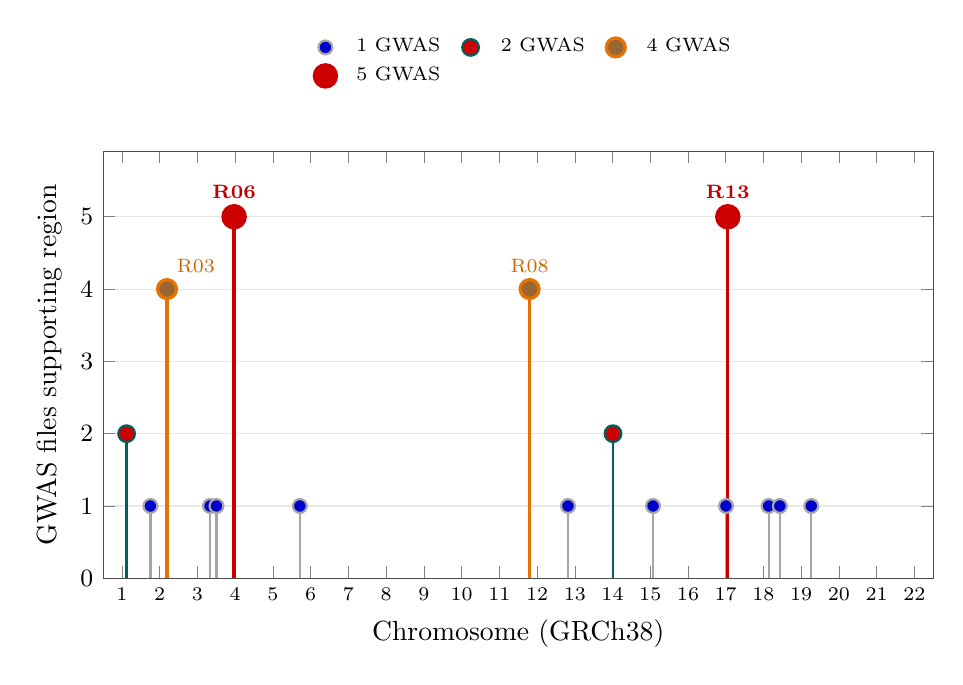
\begin{tikzpicture}
\begin{axis}[
    width=\textwidth,
    height=7.0cm,
    xmin=0.5,xmax=22.5,
    ymin=0,ymax=5.9,
    xlabel={Chromosome (GRCh38)},
    ylabel={GWAS files supporting region},
    xtick={1,2,3,4,5,6,7,8,9,10,11,12,13,14,15,16,17,18,19,20,21,22},
    ytick={0,1,2,3,4,5},
    x tick label style={font=\scriptsize},
    y tick label style={font=\small},
    ymajorgrids=true,
    grid style={gray!18},
    axis line style={black!70},
    enlarge x limits=false,
    legend style={at={(0.5,1.13)},anchor=south,legend columns=3,
                  font=\scriptsize,draw=none},
    clip=false
]
% F=1: ten single-study regions.
\addplot+[ycomb,mark=*,mark size=2.5pt,thick,gray!70]
    coordinates {
        (1.7541,1) (3.3332,1) (3.5050,1)
        (5.7150,1) (12.8194,1) (15.0737,1)
        (17.0062,1) (18.1363,1) (18.4344,1) (19.2661,1)
    };
\addlegendentry{1 GWAS}
% F=2: two repeated regions.
\addplot+[ycomb,mark=*,mark size=3pt,thick,teal!75!black]
    coordinates {(1.1235,2) (14.0126,2)};
\addlegendentry{2 GWAS}
% F=4: two high-recurrence regions.
\addplot+[ycomb,mark=*,mark size=3.4pt,very thick,orange!90!black]
    coordinates {(2.1949,4) (11.8027,4)};
\addlegendentry{4 GWAS}
% F=5: two highest-recurrence regions.
\addplot+[ycomb,mark=*,mark size=4pt,very thick,red!80!black]
    coordinates {(3.9720,5) (17.0541,5)};
\addlegendentry{5 GWAS}
\node[font=\scriptsize,anchor=south west,orange!80!black]
    at (axis cs:2.1949,4.10) {R03};
\node[font=\scriptsize,anchor=south,orange!80!black]
    at (axis cs:11.8027,4.10) {R08};
\node[font=\scriptsize\bfseries,anchor=south,red!75!black]
    at (axis cs:3.9720,5.12) {R06};
\node[font=\scriptsize\bfseries,anchor=south,red!75!black]
    at (axis cs:17.0541,5.12) {R13};
\end{axis}
\end{tikzpicture}
\caption{Manhattan-style genome-wide recurrence map of the 16
cross-study merged physical regions. The horizontal axis positions
each regional midpoint proportionally within its GRCh38 chromosome;
chromosomes occupy equal display widths. The vertical axis counts
GWAS accessions containing an overlapping fine-mapped locus, not
$-\log_{10}(P)$. Red indicates the two most recurrent regions
(R06, chr4; R13, chr17; five GWAS each), and orange marks R03
(chr2) and R08 (chr12), each observed in four GWAS.}
\label{fig:finemap_recurrence_manhattan}
\end{figure}

These recurrent regions indicate that several related GWAS analyses
implicate overlapping genomic intervals. They do not establish that
the same lead allele or causal variant was selected in every study,
nor do they provide independent replication because some GWAS use
related phenotypes and potentially overlapping cohorts. The
posterior prioritisation and QC of the study-specific fine-mapping
results should therefore be evaluated separately from regional
recurrence frequency.

\subsubsection{Output for downstream molecular interpretation}

The fine-mapping stage generated variant-level
posterior probabilities, credible-set memberships,
locus definitions and quality-control diagnostics.

These outputs provide the variant-level statistical
evidence required for the subsequent stages of
GWAS2Mech, including functional variant annotation,
molecular QTL colocalisation and prioritisation
of candidate disease-associated genes.

Fine-mapping alone does not identify the molecular
mechanism of disease association.

Instead, the prioritised variants are carried forward
for integration with regulatory annotations,
transcriptomic and other molecular QTL evidence,
and additional functional genomic resources.




% ------------------------------------------------------------------
% GWAS2Mech STEP 08: FUNCTIONAL ANNOTATION
% Drop in AFTER the fine-mapping section of the manuscript.
%
% REQUIRED IN MAIN DOCUMENT PREAMBLE (add only if not already loaded):
% \usepackage{booktabs,longtable,array,graphicx,pdflscape}
% \usepackage{amsmath}
% \usepackage{pgfplots}
% \pgfplotsset{compat=1.18}
%
% Citation keys: McLaren2016, Rentzsch2019, Cheng2023,
% Landrum2018, ENCODE2020. Add these to the manuscript .bib file.
% ------------------------------------------------------------------

\subsection{Functional annotation of fine-mapped variants (workflow step 8)}
\label{sec:functional_annotation}

\subsubsection{Functional annotation resources and reference datasets}
\label{subsec:annotation_resources}

All variants retained for fine-mapping were functionally annotated
at the variant level against local, GRCh38-compatible resources
(Table~\ref{tab:step08_annotation_resources}). The use of
\texttt{scope=all} meant that annotation was not restricted to the
original lead variants or to variants in 95\% credible sets.
The final column reports annotation availability or a positive
interval overlap in the 448 study-specific credible-set variant
records; it is not the number of independently validated functional
variants.

\begingroup
\footnotesize
\setlength{\tabcolsep}{3pt}
\renewcommand{\arraystretch}{1.13}
\begin{longtable}{@{}p{2.45cm}p{5.65cm}p{3.25cm}p{2.10cm}@{}}
\caption{Functional annotation resources integrated in GWAS2Mech
Step~08. All resources were used for variant-level or gene-level
annotations within the eight fine-mapped GWAS datasets. The coverage
column refers to the 448 study-specific 95\% credible-set variant
records. Positive interval overlaps and database matches are
distinguished from nonmissing numerical scores.}
\label{tab:step08_annotation_resources}\\
\toprule
\textbf{Resource (release)} &
\textbf{Information retrieved} &
\textbf{Example output / interpretation} &
\textbf{Observed credible-set coverage}\\
\midrule
\endfirsthead
\multicolumn{4}{l}{\textit{Table \thetable\ continued}}\\
\toprule
\textbf{Resource (release)} &
\textbf{Information retrieved} &
\textbf{Example output / interpretation} &
\textbf{Credible-set coverage}\\
\midrule
\endhead
\bottomrule
\endfoot

Ensembl VEP
(release 116; GRCh38) \cite{McLaren2016} &
Transcript-level consequences, representative consequence, gene
assignment, coding and splicing context, HGVS descriptions,
SIFT/PolyPhen predictions when applicable. &
Consequence term; functional category; gene symbol; HGVSc/HGVSp. &
Consequence: 404/448; gene: 214/448\\

CADD
(v1.7; SNVs and indels) \cite{Rentzsch2019} &
Sequence-variant deleteriousness predictions using locally
indexed SNV and indel reference data. &
Raw and PHRED scores; high-score flag at PHRED $\geq 20$. &
Score: 448/448\\

AlphaMissense
(hg38 precomputed) \cite{Cheng2023} &
Predicted pathogenicity score and class for eligible
missense substitutions; not a genome-wide consequence score. &
Pathogenicity score; likely benign, ambiguous, or likely
pathogenic class. &
Score: 2/448\\

ClinVar
(local GRCh38 VCF) \cite{Landrum2018} &
Allele-matched clinical significance, reported conditions,
and review information from the locally stored release. &
Clinical significance; pathogenic/likely pathogenic
indicator. &
Database records: 17/448\\

ENCODE SCREEN
(cCRE V4) \cite{ENCODE2020} &
Overlap with candidate cis-regulatory elements, including
promoter-like and enhancer-like elements and accessible/
CTCF-associated elements. &
Candidate cis-regulatory element (cCRE) class;
PLS, pELS, dELS, CA, etc. &
Overlapping: 99/448\\

UCSC phyloP
(100-way; hg38) &
Base-wise evolutionary conservation inferred from vertebrate
multiple-sequence alignments. &
phyloP score; conservation flag at score $\geq 2$. &
Score: 446/448\\

gnomAD population
frequencies
(via VEP) &
Variant population allele frequencies obtained from the
available VEP-linked population-frequency annotations,
including non-Finnish European frequency when present. &
Overall and ancestry-specific allele-frequency fields. &
Frequency: 419/448\\

gnomAD gene
constraint (v4.1) &
Gene-level selective constraint attached to VEP-mapped
genes, including loss-of-function intolerance and
missense constraint. &
LOEUF, pLI, missense Z-score. &
Constraint: 206/448\\

RegulomeDB
(v2.2; local GRCh38) &
Regulatory ranks, probabilities, and evidence for matching
alleles from the local, dbSNP153 common-SNV resource;
rare variants and some indels may have no entry. &
Rank 1a--7; probability; strong rank
1a--1f or 2a--2f. &
Rank: 417/448;
strong: 229/448\\

\end{longtable}
\endgroup

The high-level functional classifications were produced by VEP,
whereas CADD, AlphaMissense, ClinVar, ENCODE cCREs, phyloP,
gnomAD, and RegulomeDB supplied complementary predictive,
clinical, evolutionary, population, and regulatory annotations.
Of the 448 credible-set records, 229 (51.12\%) carried a
pipeline-defined strong RegulomeDB rank, and 99 (22.10\%)
overlapped an ENCODE cCRE. AlphaMissense covered two
missense records and should not be interpreted as providing
a negative prediction for the remaining non-missense records.
The 1000 Genomes 30$\times$ European panel was the LD reference
used during Step~06 fine-mapping and was \emph{not} an additional
functional annotation database in Step~08.

\subsubsection{Variant-level annotation strategy}

To connect statistical fine-mapping with potential molecular
mechanisms, we functionally annotated the variants retained
within the SuSiE-RSS fine-mapping regions. Annotation was
performed at the \emph{individual variant} level, rather than
solely for the LD-clumping lead variants or the genomic loci.
For each of the eight GWAS datasets with eligible loci, Step~08
used the study-specific Step~06 fine-mapping table with
\texttt{scope=all}, retaining the harmonised chromosome,
GRCh38 position, reference and alternative alleles, locus
identifier, posterior inclusion probability (PIP), and
95\% credible-set membership.

Annotations were first retrieved by genomic variant key
(chromosome, position, reference allele and alternative allele), and then
joined to the fine-mapping records for each study. Thus, the
same physical variant could appear in multiple GWAS analyses
with identical reference annotations but different association
statistics, PIPs, and credible-set memberships. The European
1000 Genomes high-coverage 30$\times$ reference panel supplied
the LD information at the \emph{fine-mapping} stage; the functional
annotations were obtained separately from local GRCh38
reference resources.

Predicted molecular consequences were obtained using Ensembl
Variant Effect Predictor (VEP) release~116 with its offline
GRCh38 cache \cite{McLaren2016}. The pipeline extracted
transcript-level consequences, the selected representative
consequence, gene identifier and symbol, transcript information,
and HGVS descriptions when available. Functional categories
were assigned using the pipeline's consequence classification:
\texttt{CODING}, \texttt{SPLICING}, \texttt{UTR},
\texttt{INTRONIC}, \texttt{NONCODING\_RNA}, \texttt{UPSTREAM},
\texttt{DOWNSTREAM}, and \texttt{OTHER}. These categories were
mutually exclusive for the summary tables, whereas the
underlying VEP consequence terms could overlap across transcripts.

Additional annotations were incorporated from CADD v1.7
(SNV and indel scores) \cite{Rentzsch2019}, AlphaMissense
missense predictions \cite{Cheng2023}, ClinVar clinical
classifications \cite{Landrum2018}, ENCODE SCREEN version~4
candidate cis-regulatory elements (cCREs) \cite{ENCODE2020},
UCSC phyloP 100-way conservation scores, gnomAD allele
frequencies and gene-level constraint metrics, and local
RegulomeDB version~2.2 regulatory evidence. The annotation
output retained source-specific scores and classifications;
no composite functional causality score was inferred.

\subsubsection{Functional evidence definitions and denominators}

Protein-altering variants were identified from the VEP
consequence categories, including missense and predicted
loss-of-function (LoF) consequences. The prespecified
annotation flags included CADD PHRED $\geq20$,
AlphaMissense \texttt{likely\_pathogenic}, ClinVar
pathogenic/likely pathogenic (excluding conflicting
classifications according to the implemented rule), phyloP
100-way $\geq2$, overlap with an ENCODE cCRE, and
RegulomeDB rankings classified by the pipeline as strong
(rank classes 1a--1f or 2a--2f).
These are source-specific annotation indicators and
should not be interpreted as independent experimental
validation of molecular activity.

The main functional interpretation focused on the variants
retained within the nominal 95\% SuSiE-RSS credible sets,
while the full annotated variant collection was retained
for comparison and downstream analyses. For functional
category $k$, the reported credible-set proportion was

\begin{equation}
 f_k = \frac{n_{k,\mathrm{CS}}}{N_{\mathrm{CS}}},
 \qquad N_{\mathrm{CS}}=448,
\end{equation}

where $n_{k,\mathrm{CS}}$ counts study-specific credible-set
variant records assigned to category $k$. The 448 records
are not 448 independent causal variants: recurrent variants
can appear in multiple studies, and several variants may
belong to the same credible set. The denominator for
annotation-source coverage similarly refers to records
with a nonmissing field or a positive interval overlap,
not the total number of possible predictions for the
variant's biological class.

\subsubsection{Annotation yield across GWAS datasets}

Of the 17 original GWAS datasets, eight had fine-mapped loci
and completed Step~08 functional annotation; the remaining
nine had no eligible fine-mapped loci and were skipped.
Across the eight datasets, 204,683 study-specific
fine-mapped variant records were annotated in 32
study-specific loci. These records corresponded to
103,881 distinct genomic variant keys across datasets.

A total of 69 nominal 95\% credible sets were reported
by fine-mapping. Their retained variant annotations
comprised 448 study-specific records representing
219 distinct genomic variant keys. At least one
credible-set variant was present in 19 of the 32 loci;
13 loci had no retained credible-set variants.
Across the 219 distinct credible-set variant keys,
136 were represented in two or more GWAS datasets.
Recurrence indicates overlap among the analysed GWAS
results and must not automatically be interpreted as
replication in independent samples.

Table~\ref{tab:step08_studies} reports the annotation yield
and selected functional evidence separately for each dataset.

\begin{table}[htbp]
\centering
\small
\setlength{\tabcolsep}{4pt}
\caption{Step~08 study-level annotation results. All counts
refer to study-specific variant records. A 95\% credible-set
(CS) variant is a retained variant record flagged by SuSiE-RSS.
The PIP threshold is $\geq0.9$. cCRE denotes overlap with an
ENCODE candidate cis-regulatory element; RDB denotes the
pipeline-defined RegulomeDB 1--2 evidence flag.}
\label{tab:step08_studies}
\resizebox{\textwidth}{!}{%
\begin{tabular}{@{}lrrrrrrr@{}}
\toprule
GWAS accession & Loci & All variants & CS variants & PIP $\geq0.9$ & CS coding & CS cCRE & CS RDB \\
\midrule
GCST90000015 & 4 & 23,861 & 0 & 0 & 0 & 0 & 0 \\
GCST90042668 & 1 & 4,267 & 0 & 0 & 0 & 0 & 0 \\
GCST90042681 & 2 & 14,601 & 13 & 6 & 0 & 4 & 9 \\
GCST90319903 & 7 & 43,535 & 75 & 16 & 1 & 20 & 41 \\
GCST90473307 & 8 & 49,610 & 89 & 11 & 1 & 17 & 43 \\
GCST90475830 & 4 & 28,943 & 28 & 11 & 0 & 10 & 15 \\
GCST90476961 & 4 & 26,557 & 129 & 7 & 0 & 27 & 66 \\
GCST90476962 & 2 & 13,309 & 114 & 1 & 0 & 21 & 55 \\
\midrule
\textbf{Total} & \textbf{32} & \textbf{204,683} & \textbf{448} & \textbf{52} & \textbf{2} & \textbf{99} & \textbf{229} \\
\bottomrule
\end{tabular}%
}
\end{table}

\subsubsection{Predominance of noncoding functional consequences}

Among the 448 credible-set variant records, 197
(43.97\%) were assigned to \texttt{NONCODING\_RNA}
and 170 (37.95\%) to \texttt{INTRONIC} categories,
collectively accounting for 367 records (81.92\%).
The remaining categories comprised 44 \texttt{OTHER}
(9.82\%), 22 \texttt{UPSTREAM} (4.91\%), seven
\texttt{UTR} (1.56\%), six \texttt{DOWNSTREAM}
(1.34\%), and two \texttt{CODING} (0.45\%) records.
No credible-set record was assigned to the pipeline's
\texttt{SPLICING} category.

The exclusive category \texttt{NONCODING\_RNA}
should not be interpreted as disjoint from an intronic
\emph{VEP consequence}: for example, a variant can be
intronic in a noncoding transcript and be classified as
\texttt{NONCODING\_RNA} by the pipeline. At the level
of potentially overlapping VEP terms, \texttt{intron\_variant}
was recorded 360 times (80.36\% of 448 records) and
a noncoding-transcript VEP consequence 190 times
(42.41\%). Because VEP terms can co-occur, the
percentages of these detailed terms need not sum to 100\%.

Table~\ref{tab:step08_category_by_study} reports the
functional classification for each study, and
Table~\ref{tab:step08_category_overall} provides the
overall comparison between the complete annotated
variant collection and the credible-set subset.

\begin{table}[htbp]
\centering
\scriptsize
\setlength{\tabcolsep}{3pt}
\caption{Functional categories of 95\% credible-set variant
records within each GWAS. Categories are mutually exclusive
by the Step~08 classification procedure; zero denotes no
record assigned to that category. NC RNA, noncoding RNA.}
\label{tab:step08_category_by_study}
\resizebox{\textwidth}{!}{%
\begin{tabular}{@{}lrrrrrrrr@{}}
\toprule
GWAS & NC RNA & Intronic & Other & Upstream & Downstream & UTR & Coding & Total \\
\midrule
GCST90000015 & 0 & 0 & 0 & 0 & 0 & 0 & 0 & 0 \\
GCST90042668 & 0 & 0 & 0 & 0 & 0 & 0 & 0 & 0 \\
GCST90042681 & 3 & 4 & 5 & 0 & 0 & 1 & 0 & 13 \\
GCST90319903 & 13 & 42 & 10 & 7 & 1 & 1 & 1 & 75 \\
GCST90473307 & 43 & 33 & 7 & 3 & 1 & 1 & 1 & 89 \\
GCST90475830 & 9 & 6 & 9 & 0 & 3 & 1 & 0 & 28 \\
GCST90476961 & 67 & 40 & 13 & 6 & 1 & 2 & 0 & 129 \\
GCST90476962 & 62 & 45 & 0 & 6 & 0 & 1 & 0 & 114 \\
\midrule
\textbf{Total} & \textbf{197} & \textbf{170} & \textbf{44} & \textbf{22} & \textbf{6} & \textbf{7} & \textbf{2} & \textbf{448} \\
\bottomrule
\end{tabular}%
}
\end{table}

\begin{table}[htbp]
\centering
\small
\caption{Functional consequence composition in the full
annotated collection and in the 95\% credible-set subset.
All values count study-specific records. The percentage column
uses the 448 credible-set records as denominator.}
\label{tab:step08_category_overall}
\begin{tabular}{@{}lrrr@{}}
\toprule
Functional class & All annotated & CS variants & CS (\%) \\
\midrule
Noncoding RNA & 46,137 & 197 & 43.97 \\
Intronic & 108,582 & 170 & 37.95 \\
Other/unassigned & 27,386 & 44 & 9.82 \\
Upstream & 9,197 & 22 & 4.91 \\
Untranslated region & 3,189 & 7 & 1.56 \\
Downstream & 7,316 & 6 & 1.34 \\
Coding & 2,386 & 2 & 0.45 \\
Splicing & 490 & 0 & 0.00 \\
\midrule
\textbf{Total} & \textbf{204,683} & \textbf{448} & \textbf{100.00} \\
\bottomrule
\end{tabular}
\end{table}

\subsubsection{Regulatory, deleteriousness, and clinical annotations}

Of the 448 credible-set variant records, 99 (22.10\%)
overlapped ENCODE cCREs, while 229 (51.12\%)
met the pipeline-defined strong RegulomeDB criterion.
Five records (1.12\%) met the phyloP conservation
threshold of at least 2. In contrast, no credible-set
record reached CADD PHRED $\geq20$, was classified
as AlphaMissense likely pathogenic, or carried an
unconflicted pathogenic/likely pathogenic ClinVar flag
under the implemented annotation rules.
These features are not exclusive: a single variant
may overlap a cCRE and also have a RegulomeDB flag.

The restriction to credible sets substantially changed
these functional counts relative to all fine-mapped
variant records. For example, 652 records in the full
annotation collection had CADD PHRED $\geq20$ and
84 had a pipeline-defined LoF consequence, but none
of these records belonged to the retained 95\%
credible-set variant subset. The lack of such evidence
within the CS subset is not evidence that the associated
regions lack biological function.

\begin{figure}[htbp]
\centering
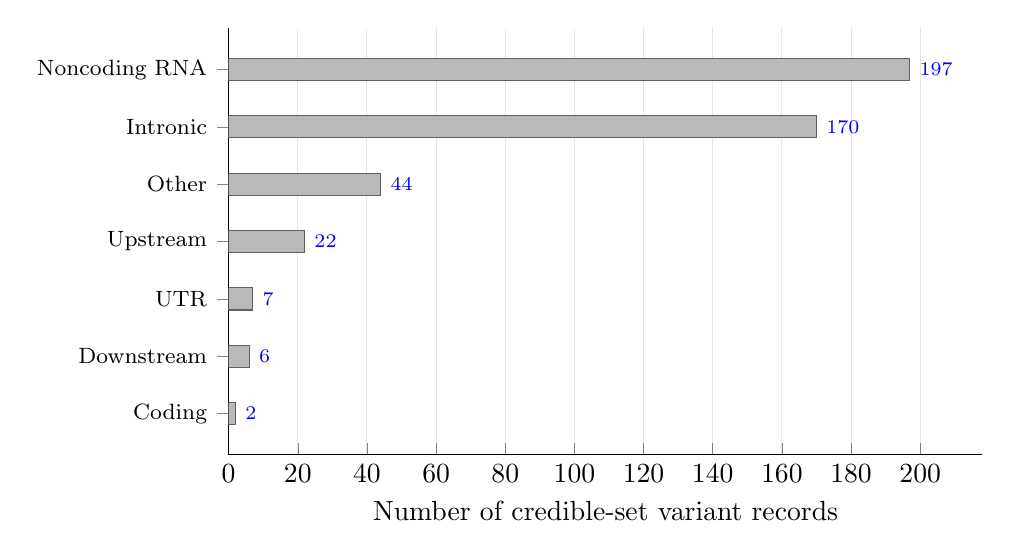
\begin{tikzpicture}
\begin{axis}[
  xbar,
  width=0.92\textwidth,
  height=7cm,
  xmin=0,xmax=218,
  xlabel={Number of credible-set variant records},
  symbolic y coords={Coding,Downstream,UTR,Upstream,Other,Intronic,Noncoding RNA},
  ytick=data,
  yticklabel style={font=\footnotesize},
  nodes near coords,
  nodes near coords align={horizontal},
  every node near coord/.append style={font=\scriptsize},
  bar width=8pt,
  axis x line*=bottom,
  axis y line*=left,
  xmajorgrids=true,
  grid style={gray!20},
  enlarge y limits=0.12
]
\addplot+[fill=gray!55,draw=gray!75!black] coordinates {
 (2,Coding) (6,Downstream) (7,UTR) (22,Upstream)
 (44,Other) (170,Intronic) (197,Noncoding RNA)
};
\end{axis}
\end{tikzpicture}
\caption{Mutually exclusive Step~08 functional categories
among the 448 study-specific 95\% credible-set variant
records. The noncoding RNA category can nevertheless
include VEP intron-variant terms on noncoding transcripts.}
\label{fig:step08_consequence_bar}
\end{figure}

\begin{table}[htbp]
\centering
\small
\caption{Functional annotation flags in the full
fine-mapped variant collection versus the 95\% credible-set
subset. Flags are non-exclusive. RegulomeDB 1--2 indicates
the implemented ranking rule, rather than experimentally
confirmed causal regulatory effects.}
\label{tab:step08_evidence}
\begin{tabular}{@{}lrrr@{}}
\toprule
Annotation criterion & All records & CS records & CS (\%) \\
\midrule
Loss of function & 84 & 0 & 0.00 \\
Coding & 2,470 & 2 & 0.45 \\
Missense & 1,214 & 2 & 0.45 \\
Splicing & 490 & 0 & 0.00 \\
CADD PHRED $\geq20$ & 652 & 0 & 0.00 \\
AlphaMissense likely pathogenic & 26 & 0 & 0.00 \\
ClinVar pathogenic/likely pathogenic & 1 & 0 & 0.00 \\
ENCODE cCRE overlap & 51,615 & 99 & 22.10 \\
phyloP 100-way $\geq2$ & 2,718 & 5 & 1.12 \\
RegulomeDB strong (1--2) & 92,025 & 229 & 51.12 \\
\bottomrule
\end{tabular}
\end{table}

\subsubsection{Annotation completeness and resource coverage}

The completeness of annotation differed by resource and
type of functional effect. CADD PHRED was available
for all 448 credible-set records, phyloP scores for
446 (99.55\%), RegulomeDB rankings for 417 (93.08\%),
and gnomAD population allele frequencies for 419
(93.53\%). A representative VEP consequence was
available for 404 (90.18\%), while a selected VEP gene
symbol was available for 214 (47.77\%).

AlphaMissense values were present for only two
credible-set records; both represented the same
missense variant in separate studies. This is expected
to be a highly consequence-dependent resource, so
availability relative to all 448 variants should not be
used as a measure of its accuracy or completeness for
eligible missense substitutions. Likewise, a missing
gene symbol or empty representative VEP consequence
is not evidence that a variant is biologically inert.

The local annotation provenance recorded successful
resource access for CADD, AlphaMissense, ClinVar,
ENCODE cCRE, phyloP, RegulomeDB, and gnomAD gene
constraint across eight datasets. The VEP provenance
status field was reported as \texttt{UNKNOWN} by the
audit; nevertheless, VEP consequence fields were
present for 404 credible-set records. The VEP status
field should therefore be treated as an incomplete
audit-status field rather than an indication that VEP
was unavailable or failed.

\begin{table}[htbp]
\centering
\small
\caption{Coverage of annotation fields among all
fine-mapped records and the 95\% credible-set subset.
Coverage reflects nonmissing values, except cCRE where
it represents a positive interval overlap; consequently,
the cCRE row is an overlap count rather than an assay
availability estimate.}
\label{tab:step08_coverage}
\begin{tabular}{@{}lrrrr@{}}
\toprule
Annotation field & All $n$ & All (\%) & CS $n$ & CS (\%) \\
\midrule
VEP representative consequence & 177,297 & 86.6 & 404 & 90.2 \\
VEP selected gene symbol & 145,064 & 70.9 & 214 & 47.8 \\
CADD PHRED score & 204,679 & 100.0 & 448 & 100.0 \\
AlphaMissense score & 852 & 0.4 & 2 & 0.4 \\
ClinVar classification & 4,638 & 2.3 & 17 & 3.8 \\
ENCODE cCRE overlap & 51,615 & 25.2 & 99 & 22.1 \\
phyloP 100-way score & 203,418 & 99.4 & 446 & 99.6 \\
RegulomeDB ranking & 192,612 & 94.1 & 417 & 93.1 \\
gnomAD allele frequency & 194,339 & 94.9 & 419 & 93.5 \\
gnomAD gene constraint & 126,012 & 61.6 & 206 & 46.0 \\
\bottomrule
\end{tabular}
\end{table}

\subsubsection{Locus-level annotation and candidate variants}

The 32 study-specific loci contained between 3,722
and 9,332 annotated variant records each in the
observed run. Table~\ref{tab:step08_locus_master}
reports every locus, its annotated variant count,
number of variants retained in nominal 95\% credible
sets, highest-PIP record and representative VEP gene
and consequence. The top variant is selected using
PIP across \emph{all} annotated regional variants;
it is not necessarily a member of a retained credible
set. Moreover, the absence of a credible set does not
imply the absence of a strong marginal association.

% --------------------------------------------------------------
% FULL 32-LOCUS TABLE, LANDSCAPE, AUTOMATIC PAGE BREAKS
% --------------------------------------------------------------
\begin{landscape}
\begingroup
\scriptsize
\setlength{\tabcolsep}{3.7pt}
\renewcommand{\arraystretch}{1.10}
\begin{longtable}{@{}llrrllrlp{4.0cm}@{}}
\caption{Complete study-specific functional annotation summary
for the 32 fine-mapped loci. $N$ is the number of variant
records annotated at that locus; CS is the number of variants
marked as members of 95\% credible sets; $N_{0.9}$ is the
number of records with PIP $\geq0.9$. The reported gene and
consequence are the selected representative VEP annotation
of the top-PIP variant, not an established causal target.}
\label{tab:step08_locus_master}\\
\toprule
GWAS & Locus & $N$ & CS & Top variant/rsID & PIP & $N_{0.9}$ & Gene & VEP consequence \\
\midrule
\endfirsthead
\multicolumn{9}{l}{\textit{Table continued from previous page}}\\
\toprule
GWAS & Locus & $N$ & CS & Top variant/rsID & PIP & $N_{0.9}$ & Gene & VEP consequence \\
\midrule
\endhead
\midrule\multicolumn{9}{r}{\textit{Continued on next page}}\\
\endfoot
\bottomrule
\endlastfoot
GCST90000015 & L001 & 5,737 & 0 & \texttt{6:35726373:G:A} & 0.0000 & 0 & -- & downstream gene \\
GCST90000015 & L002 & 6,295 & 0 & \texttt{15:57805106:G:A} & 0.0135 & 0 & -- & -- \\
GCST90000015 & L003 & 5,075 & 0 & \texttt{18:51304051:C:T} & 0.0142 & 0 & -- & -- \\
GCST90000015 & L004 & 6,754 & 0 & \texttt{18:75158255:C:G} & 0.0190 & 0 & -- & intron; noncoding transcript \\
GCST90042668 & L001 & 4,267 & 0 & \texttt{17:41147152:G:C} & 0.0000 & 0 & KRTAP4-5 & downstream gene \\
GCST90042681 & L001 & 6,485 & 0 & \texttt{12:40795186:C:A} & 0.0402 & 0 & CNTN1 & intron \\
GCST90042681 & L002 & 8,116 & 13 & \texttt{17:46026338:G:A} & 1.0000 & 6 & MAPT & 3' UTR \\
GCST90319903 & L001 & 3,722 & 4 & \texttt{rs2230288} & 0.4927 & 0 & GBA1 & missense \\
GCST90319903 & L002 & 5,999 & 6 & \texttt{rs9917256} & 1.0000 & 6 & -- & -- \\
GCST90319903 & L003 & 6,734 & 29 & \texttt{rs356219} & 0.9260 & 1 & -- & intron; noncoding transcript \\
GCST90319903 & L004 & 6,832 & 0 & \texttt{rs1491942} & 0.0292 & 0 & LRRK2 & intron \\
GCST90319903 & L005 & 5,954 & 26 & \texttt{rs7155501} & 0.2504 & 0 & GCH1 & intron \\
GCST90319903 & L006 & 8,375 & 10 & \texttt{rs16940802} & 1.0000 & 8 & MAPT & 3' UTR \\
GCST90319903 & L007 & 5,919 & 0 & \texttt{rs429358} & 0.9474 & 1 & APOE & missense \\
GCST90473307 & L001 & 3,819 & 4 & \texttt{rs2230288} & 0.6455 & 0 & GBA1 & missense \\
GCST90473307 & L002 & 6,251 & 6 & \texttt{rs6722770} & 0.9351 & 1 & -- & intron; noncoding transcript \\
GCST90473307 & L003 & 6,112 & 0 & \texttt{rs1086091} & 0.0000 & 0 & -- & -- \\
GCST90473307 & L004 & 6,512 & 1 & \texttt{rs11248057} & 0.9722 & 1 & GAK & intron \\
GCST90473307 & L005 & 6,971 & 56 & \texttt{rs356219} & 0.6625 & 0 & -- & intron; noncoding transcript \\
GCST90473307 & L006 & 6,849 & 0 & \texttt{rs117463377} & 0.0523 & 0 & KIF21A & intron \\
GCST90473307 & L007 & 6,223 & 13 & \texttt{rs2183081} & 0.1643 & 0 & GCH1 & intron \\
GCST90473307 & L008 & 6,873 & 9 & \texttt{rs2668679} & 1.0000 & 9 & -- & intron; noncoding transcript \\
GCST90475830 & L001 & 6,204 & 6 & \texttt{rs9917256} & 1.0000 & 6 & -- & -- \\
GCST90475830 & L002 & 6,397 & 13 & \texttt{rs356183} & 0.3641 & 0 & -- & intron; noncoding transcript \\
GCST90475830 & L003 & 7,010 & 0 & \texttt{rs1874558} & 0.0511 & 0 & SLC2A13 & intron \\
GCST90475830 & L004 & 9,332 & 9 & \texttt{rs566242433} & 1.0000 & 5 & -- & -- \\
GCST90476961 & L001 & 7,572 & 0 & \texttt{rs139198918} & 0.4801 & 0 & -- & intron; noncoding transcript \\
GCST90476961 & L002 & 6,205 & 17 & \texttt{rs9917256} & 0.1591 & 0 & -- & -- \\
GCST90476961 & L003 & 6,397 & 103 & \texttt{rs356182} & 0.4186 & 0 & -- & intron; noncoding transcript \\
GCST90476961 & L004 & 6,383 & 9 & \texttt{rs566242433} & 1.0000 & 7 & -- & -- \\
GCST90476962 & L001 & 6,398 & 114 & \texttt{rs356182} & 0.9565 & 1 & -- & intron; noncoding transcript \\
GCST90476962 & L002 & 6,911 & 0 & \texttt{rs145240445} & 0.0072 & 0 & -- & -- \\
\end{longtable}
\endgroup
\end{landscape}

\subsubsection{Representative variants and biological interpretation}

Functional annotation implicated both protein-coding
and regulatory candidate mechanisms, with marked
variation in statistical support across studies.
At the chromosome~1 \textit{GBA1} region,
\texttt{rs2230288} (GRCh38 chr1:155,236,376:C:T)
was annotated as a missense variant in both
GCST90319903 (PIP 0.4927) and GCST90473307
(PIP 0.6455). Both records were included in
credible sets and together accounted for the
two coding/missense credible-set \emph{records}
reported in Table~\ref{tab:step08_evidence};
there was one distinct missense variant key.
Its CADD PHRED score was 19.46, AlphaMissense
classified it as \texttt{likely\_benign}, and
ClinVar reported conflicting classifications,
including risk-factor interpretations. These
heterogeneous annotations should not be collapsed
into a single pathogenicity claim.

In the chromosome~17 \textit{MAPT} region,
\texttt{rs16940802} (chr17:46,026,338:G:A)
was annotated as a 3$'$-UTR variant with
PIP 1.0000 in GCST90319903 and an overlapping
ENCODE distal enhancer-like element (dELS)
with a RegulomeDB 1f ranking. The same
GRCh38 variant key was also detected in
GCST90042681 with PIP 1.0000; the
saved primary rsID field was missing for
that study. These are study-specific statistical
results, not two validated independent signals.

A chromosome~4 \textit{GAK} intronic variant,
\texttt{rs11248057}, had PIP 0.9722 in
GCST90473307 and overlapped an ENCODE dELS,
with a RegulomeDB 1f annotation. In the
chromosome~4 region encompassing
\textit{SNCA}-related candidate signals,
\texttt{rs356182} had PIPs of 0.0374,
0.4186, and 0.9565 across GCST90475830,
GCST90476961, and GCST90476962, respectively.
It was annotated as an intronic/noncoding-transcript
variant with promoter-proximal enhancer-like
(pELS) overlap and RegulomeDB 1f evidence.
Differences in PIP across GWAS studies reflect
differences in summary statistics and fine-mapping
models rather than differences in the reference
functional annotation of the variant.

The chromosome~2 \texttt{rs9917256} variant
was retained in credible sets from four GWAS
datasets and attained PIP 1.0000 in
GCST90319903 and GCST90475830; despite
its strong statistical support, the output
contained no representative VEP consequence or
selected gene symbol (functional class
\texttt{OTHER}). Such observations illustrate why
statistical fine-mapping confidence and functional
annotation completeness must be evaluated separately.

Conversely, the \textit{APOE} missense variant
\texttt{rs429358} attained PIP 0.9474 in
GCST90319903 locus L007, but that locus
contained no retained credible-set variant
records in the saved Step~08 output. It was
therefore \emph{not} included in the credible-set
coding/missense totals. This discordance supports
the need to review SuSiE-RSS diagnostics, LD
matching, and credible-set filtering before
causal prioritisation.

\begin{table}[htbp]
\centering
\scriptsize
\setlength{\tabcolsep}{3pt}
\caption{Selected observed variants illustrating the
integration of statistical fine-mapping with functional
annotations. ``CS'' indicates whether the displayed
variant record was present in the 95\% credible-set
variant table for that GWAS; a gene symbol is the
representative annotation, not a confirmed target.}
\label{tab:step08_example_variants}
\resizebox{\textwidth}{!}{%
\begin{tabular}{@{}lllrlp{6.0cm}@{}}
\toprule
GWAS & Variant & Selected gene & PIP & CS & Annotation/evidence \\
\midrule
GCST90319903 & rs2230288 & \textit{GBA1} & 0.4927 & Yes & Missense; CADD 19.46; conflicting ClinVar \\
GCST90473307 & rs2230288 & \textit{GBA1} & 0.6455 & Yes & Same missense variant; RegulomeDB 1f \\
GCST90319903 & rs16940802 & \textit{MAPT} & 1.0000 & Yes & 3$'$-UTR; ENCODE dELS; RegulomeDB 1f \\
GCST90473307 & rs11248057 & \textit{GAK} & 0.9722 & Yes & Intronic; ENCODE dELS; RegulomeDB 1f \\
GCST90475830 & rs356182 & -- & 0.0374 & Yes & Noncoding transcript/intronic; pELS; RegulomeDB 1f \\
GCST90476961 & rs356182 & -- & 0.4186 & Yes & Same functional annotation; different study PIP \\
GCST90476962 & rs356182 & -- & 0.9565 & Yes & Same functional annotation; different study PIP \\
GCST90319903 & rs9917256 & -- & 1.0000 & Yes & Class OTHER; missing VEP consequence; RegulomeDB 1f \\
GCST90319903 & rs429358 & \textit{APOE} & 0.9474 & No & Missense; cCRE pELS; outside retained credible sets \\
\bottomrule
\end{tabular}%
}
\end{table}

\subsubsection{Interpretation and limitations}

The functional annotation results suggest that the
fine-mapped Parkinson's disease-associated regions
are enriched in noncoding sequence annotations,
with many credible-set variants showing regulatory
evidence. However, the observed proportions describe
the selected credible-set collection and are not a
formal statistical enrichment against a matched
genomic background. The annotations also do not
establish tissue-specific enhancer activity or
identify the molecular target gene of a noncoding
variant without supporting molecular-QTL or
functional evidence.

Fine-mapping quality-control warnings must be
considered when interpreting all high-PIP variants.
In the preceding Step~06 analysis, 30 of the 32
study-specific loci carried at least one warning,
and five model fits did not converge within the
configured 500 iterations. Such locus-level warnings,
missing reference/allele matches, incomplete
representative VEP consequences, and overlapping
GWAS samples limit causal interpretation. The
functional annotations were therefore used for
hypothesis generation and prioritisation rather than
as definitive evidence of pathogenicity or a
validated disease mechanism.

The variant-level functional evidence and credible-set
memberships provide a basis for the next stage:
colocalisation against eQTL, sQTL and other molecular
QTL datasets, followed by evaluation of candidate
regulatory mechanisms and gene targets.

% GWAS2Mech: combined Step08--Step11 Methods and Results.
% Expected packages in the parent preamble:
%   \usepackage{booktabs,graphicx,array,amsmath,flafter}
% Compatible with article and two-column manuscripts (tables use table*).
% Citations require GWAS2Mech_Step08_to_Step11_Methods.bib, merged with your .bib.
%
% Scope: eight Parkinson's disease GWAS, European ancestry, 1000G30x LD reference.
% Results taken from the 2026-10-17/18 Step09--12 console logs and previously
% established Step08 annotation summaries. No causal effect is asserted.


\subsection{Molecular-QTL inputs and colocalisation framework (workflow steps 9--12)}
\label{sec:functional_annotation_coloc}

\subsubsection{Variant annotation inputs to molecular-QTL integration}
\label{subsec:functional_annotation}

\paragraph{Methodology.}

Following GWAS locus identification and SuSiE-RSS fine-mapping,
we performed comprehensive functional annotation to characterise
the potential biological consequences of variants associated
with Parkinson's disease.

Fine-mapped variants were annotated using Ensembl Variant
Effect Predictor (VEP, release 116) against the GRCh38 human
reference genome. Complementary resources included CADD,
AlphaMissense, ClinVar, ENCODE candidate cis-regulatory elements
(cCREs), phyloP, RegulomeDB, and gnomAD population-frequency
and gene-constraint annotations.

For each variant, the pipeline retained its genomic position,
reference and alternative alleles, GWAS study, locus identifier,
posterior inclusion probability (PIP), credible-set membership,
predicted functional consequence, gene annotations, and
available functional evidence.

The primary variant-level prioritisation focused on variants
belonging to the SuSiE-RSS 95\% credible sets. However,
annotation was also performed on the broader collection
of fine-mapped variants to preserve regional biological
information.

\begin{table*}[t]
\centering
\caption{Functional annotation resources incorporated into
GWAS2Mech. The final column reports available annotation
records among the 448 study-specific GWAS credible-set
variant records. Some variants occur in multiple GWAS studies.
Versions should be verified against the resource provenance
records before final manuscript submission.}
\label{tab:annotation_resources}
\footnotesize
\begin{tabular}{@{}p{2.7cm}p{2.0cm}p{7.5cm}r@{}}
\toprule
Resource & Version & Information extracted & Records \\
\midrule
Ensembl VEP & 116, GRCh38
& Gene and transcript consequences, HGVS, functional effects
& 404 \\
CADD & v1.7
& Predicted deleteriousness and PHRED scores
& 448 \\
AlphaMissense & hg38
& Missense pathogenicity predictions
& 2 \\
ClinVar & GRCh38 local release
& Clinical significance and associated conditions
& 17 \\
ENCODE SCREEN & cCRE v4
& Promoter, enhancer and other candidate regulatory overlaps
& 99 \\
phyloP & 100-way
& Evolutionary conservation
& 446 \\
RegulomeDB & v2.2
& Regulatory ranking and evidence
& 417 \\
gnomAD frequencies & VEP-linked
& Population allele frequencies
& 419 \\
gnomAD constraint & v4.1
& LOEUF, pLI and missense constraint
& 206 \\
\bottomrule
\end{tabular}
\end{table*}

\paragraph{Annotation results.}

Functional annotation was completed for 204,683
study-specific fine-mapped variant records across
32 genomic loci from eight European-ancestry
Parkinson's disease GWAS datasets.

SuSiE-RSS fine-mapping had identified 69 study-specific
95\% credible sets, containing 448 study-specific
credible-set variant records. These corresponded to
219 distinct normalised variant keys across the
GWAS datasets.

The functional classification of credible-set variants
was dominated by noncoding annotations, particularly
noncoding-RNA and intronic consequences.

\begin{table}[t]
\centering
\caption{Mutually exclusive functional classifications
of the 448 study-specific credible-set variant records.}
\label{tab:credible_set_categories}
\small
\begin{tabular}{@{}lrr@{}}
\toprule
Functional category & Variants & Percentage (\%) \\
\midrule
Noncoding RNA & 197 & 43.97 \\
Intronic & 170 & 37.95 \\
Other & 44 & 9.82 \\
Upstream & 22 & 4.91 \\
Untranslated region & 7 & 1.56 \\
Downstream & 6 & 1.34 \\
Coding & 2 & 0.45 \\
\midrule
Total & 448 & 100.00 \\
\bottomrule
\end{tabular}
\end{table}

Noncoding-RNA and intronic categories together accounted
for 81.92\% of the credible-set records, suggesting that
many fine-mapped disease-associated variants may
participate in noncoding regulatory processes.

Only two study-specific credible-set records were
classified as coding. Both corresponded to the
\textit{GBA1} missense variant rs2230288 represented
in separate GWAS datasets.

Among credible-set records, 99 overlapped ENCODE cCREs,
whereas 229 satisfied the pipeline-defined strong
RegulomeDB ranking criterion. Five records met the
pipeline's conservation-evidence threshold.

These functional annotations provided candidate biological
interpretations but did not independently demonstrate
regulatory activity or establish variant causality.


\subsubsection{Integration of fine-mapping and molecular-QTL data}
\label{subsec:coloc_methodology}

\paragraph{Colocalisation framework.}

To investigate potential molecular mechanisms underlying
the identified GWAS associations, we integrated GWAS
fine-mapping evidence with molecular quantitative trait
locus (QTL) datasets.

The analysis evaluated whether a disease-associated
genetic signal and a molecular phenotype were consistent
with sharing an underlying causal association signal.

Five hypotheses were considered:

\begin{align}
H_0 &: \text{Neither trait is associated}, \\
H_1 &: \text{Only the GWAS trait is associated}, \\
H_2 &: \text{Only the molecular trait is associated}, \\
H_3 &: \text{Both traits have distinct causal signals}, \\
H_4 &: \text{Both traits share a causal signal}.
\end{align}

The posterior probability of colocalisation was defined as

\begin{equation}
PP_{H4}
=
P(H_4 \mid D_{\mathrm{GWAS}},D_{\mathrm{QTL}}).
\label{eq:coloc_h4}
\end{equation}

A comparison was classified as having strong
shared-signal support when

\begin{equation}
PP_{H4} \geq 0.80.
\end{equation}

Comparisons with
$0.50 \leq PP_{H4} < 0.80$
were classified as suggestive.

Sensitivity to the shared-signal prior was evaluated
using the more conservative prior
$p_{12}=10^{-6}$.

Three complementary molecular-QTL analyses were
performed, representing bulk-tissue, cell-type-specific,
and external molecular-QTL resources.


\subsection{Molecular-QTL colocalisation results and integrated evidence (workflow steps 9--12)}
\label{sec:evidence_integration}

Following functional annotation and molecular QTL
colocalisation, evidence was integrated across
GWAS studies, genomic loci, fine-mapped variants,
molecular traits, candidate genes, and biological
contexts.

The integration preserved locus identifiers,
GWAS posterior inclusion probabilities,
credible-set membership, functional annotations,
colocalisation posterior probabilities, tissue
or cell-type labels, and evidence provenance.

Bulk-tissue, cell-type-specific, and external
molecular-QTL associations were maintained as
separate evidence channels before aggregation
at the locus--gene level.

The integrated analysis produced 1,601
study-specific locus--gene evidence records
and identified 395 unique genes in the
downstream pathway-input collection.

These quantities represent computational
candidate associations and do not indicate
1,601 independent loci or 395 experimentally
validated disease genes.

Because the analyses included potentially
overlapping GWAS cohorts, multiple tissues,
repeated molecular phenotypes, and loci with
fine-mapping quality-control warnings,
evidence aggregation was used for candidate
prioritisation rather than causal confirmation.

Candidates were subsequently selected for
comparison with independent external
knowledge resources to assess concordance
with existing genetic and functional
evidence.



\subsubsection{Bulk-tissue molecular-QTL colocalisation:
Step 09}

Bulk-tissue colocalisation was performed using molecular
QTL data obtained through the eQTL Catalogue resource
snapshot, including GTEx and additional configured
datasets.

The submitted resource snapshot contained 246 QTL
contexts and supported analysis of gene expression
(eQTL), RNA splicing (sQTL), exon usage (exonQTL),
transcript isoforms (isoQTL), and available protein
QTL phenotypes.

GWAS SuSiE-RSS association components were compared
with provider-derived molecular-QTL SuSiE components
using the \texttt{coloc.bf\_bf} framework.

This signal-level approach accommodated multiple
association components within a locus.

The colocalisation analysis used regional variant-level
Bayes factor information, while the retained GWAS
credible sets defined the eligible GWAS association
components.

Loci without retained GWAS credible sets were not
eligible for this analysis.


\subsubsection{Cell-type-specific molecular-QTL
colocalisation: Step 10}

To investigate whether disease-associated genetic signals
were shared with cell-type-specific expression regulation,
we applied the signal-level colocalisation framework
to single-cell and cell-type eQTL resources.

The submitted snapshot contained 167 QTL contexts,
including data from Jerber, OneK1K, Nathan,
and Cytoimmgen studies.

GWAS and QTL fine-mapping components were compared
using \texttt{coloc.bf\_bf}, following the same
general procedure used for bulk-tissue colocalisation.

Evidence derived from bulk tissues and individual
cell types was retained separately to preserve
biological context.


\subsubsection{External molecular-QTL colocalisation:
Step 11}

Additional molecular-QTL datasets were incorporated
to evaluate RNA splicing, protein abundance,
histone-associated regulation, and chromatin accessibility.

The submitted Step 11 resource snapshot included
eight datasets spanning sQTL, pQTL, haQTL, and caQTL
modalities.

Regional GWAS and molecular-QTL association statistics
were harmonised by GRCh38 genomic position and alleles.

Following the credible-set-aware pipeline update,
only loci containing retained GWAS credible sets
were eligible for testing. Individual QTL comparisons
also required at least one allele-matched GWAS
credible-set variant.

Nevertheless, all eligible harmonised variants across
the tested regional association window were retained
for statistical colocalisation, rather than restricting
the association analysis to credible-set variants alone.

External QTL colocalisation employed the approximate
Bayes factor method, \texttt{coloc.abf}.

Unlike the multiple-signal analyses in Steps 09
and 10, this approach assumes a single causal
association signal per trait within the tested region.

The pipeline therefore recorded assumption warnings
for regions containing multiple GWAS signals or
complex linkage disequilibrium.

To assess consistency between regional colocalisation
and GWAS fine-mapping, we calculated the conditional
shared-causal-variant posterior mass within the
GWAS credible set:

\begin{equation}
M_{\mathrm{CS}\mid H4}
=
\sum_{v\in\mathcal{C}_{\mathrm{GWAS}}
\cap\mathcal{V}_{\mathrm{shared}}}
P(v\mid H_4,D_{\mathrm{GWAS}},D_{\mathrm{QTL}}).
\label{eq:credible_set_h4}
\end{equation}

Here, $\mathcal{C}_{\mathrm{GWAS}}$ represents the
GWAS credible-set variants and
$\mathcal{V}_{\mathrm{shared}}$ represents harmonised
variants available in the colocalisation analysis.

A strong external-QTL result was further prioritised
as credible-set-supported when

\begin{equation}
PP_{H4}\geq0.80
\quad \mathrm{and} \quad
M_{\mathrm{CS}\mid H4}\geq0.50.
\end{equation}

The posterior-mass threshold was applied as a
candidate-prioritisation criterion rather than
an independent statistical significance test.


\subsubsection{Molecular-QTL colocalisation results}
\label{subsec:coloc_results}

\paragraph{GWAS and credible-set coverage.}

Of the 32 study-specific GWAS loci,
19 contained at least one retained SuSiE-RSS
credible-set component and were eligible for
molecular QTL colocalisation.

The remaining 13 loci were not evaluated by the
credible-set-dependent analyses because no
GWAS credible set had been retained.

The absence of a credible set was interpreted as
a fine-mapping eligibility or uncertainty outcome,
not evidence for the absence of a molecular effect.

Table~\ref{tab:gwas_coloc_overview} presents the
study-specific fine-mapping and molecular-QTL
colocalisation results.

\begin{table*}[t]
\centering
\caption{Integration of GWAS fine-mapping, functional
annotation, and molecular-QTL colocalisation across eight
Parkinson's disease GWAS datasets.
CS, credible set; Strong, candidate molecular
trait/context comparison with $PP_{H4}\geq0.80$.
The columns count study-specific records and tests,
not independent causal variants or genes.}
\label{tab:gwas_coloc_overview}
\footnotesize
\setlength{\tabcolsep}{5pt}
\begin{tabular}{@{}lrrrrrr@{}}
\toprule
GWAS accession & Loci & CS &
CS variants & Bulk strong &
Cell strong & External strong \\
\midrule
GCST90000015 & 4 & 0 & 0 & 0 & 0 & 0 \\
GCST90042668 & 1 & 0 & 0 & 0 & 0 & 0 \\
GCST90042681 & 2 & 8 & 13 & 14 & 5 & 4 \\
GCST90319903 & 7 & 19 & 75 & 125 & 51 & 5 \\
GCST90473307 & 8 & 15 & 89 & 95 & 7 & 20 \\
GCST90475830 & 4 & 14 & 28 & 27 & 2 & 3 \\
GCST90476961 & 4 & 11 & 129 & 47 & 9 & 4 \\
GCST90476962 & 2 & 2 & 114 & 33 & 4 & 1 \\
\midrule
Total & 32 & 69 & 448 & 341 & 78 & 37 \\
\bottomrule
\end{tabular}
\end{table*}


\paragraph{Overall colocalisation evidence.}

Across the three molecular-QTL analysis stages,
35,466 candidate trait/context comparisons
were formally tested.

Of these, 456 comparisons met the strong
colocalisation threshold.

The bulk-tissue analysis contributed 341 strong
results, the cell-type analysis contributed 78,
and the external molecular-QTL analysis contributed 37.

\begin{table}[t]
\centering
\caption{Summary of molecular-QTL colocalisation
results across Steps 09--11.}
\label{tab:coloc_results_summary}
\small
\begin{tabular}{@{}lrrr@{}}
\toprule
Metric & Bulk & Cell & External \\
\midrule
Tested & 31,241 & 2,762 & 1,463 \\
Strong & 341 & 78 & 37 \\
Prior robust & 128 & 18 & 27 \\
CS-supported strong & -- & -- & 17 \\
\bottomrule
\end{tabular}
\end{table}

The number of strong colocalisation tests should
not be interpreted as the number of independent
causal loci, genes, or variants.

Multiple molecular traits, tissues, cell types,
and GWAS studies could contribute repeated
evidence for related genomic regions.


\paragraph{Bulk-tissue molecular-QTL findings.}

Step 09 completed 31,241 formal colocalisation tests,
identifying 341 strong shared-signal comparisons.

Of these strong results, 158 involved transcript
isoform QTLs, 99 involved exon QTLs,
43 involved gene-expression QTLs,
40 involved splicing QTLs, and one involved
a protein QTL.

A total of 128 strong comparisons remained
robust under the conservative shared-signal prior.

Strong bulk-tissue evidence was observed across
15 study-specific loci.

Among the notable results were molecular-QTL
signals associated with the \textit{SNCA},
\textit{MAPT}, \textit{GAK}, and
\textit{GBA1}-associated genomic regions.

For example, the \textit{SNCA} locus
(GCST90473307, L005) displayed strong
isoQTL colocalisation in adipose tissue
($PP_{H4}\approx0.998$), with additional
support in brain substantia nigra
($PP_{H4}\approx0.993$).

These findings supported candidate transcript-level
regulatory associations at the GWAS locus,
without establishing that the observed molecular
effects mediate disease risk.


\paragraph{Cell-type-specific molecular-QTL findings.}

Step 10 completed 2,762 formal colocalisation
tests and identified 78 strong eQTL
colocalisation comparisons.

Of these, 18 remained strong under the
conservative shared-signal prior.

Strong colocalisation was observed across
ten study-specific loci.

Among the strongest results, expression-QTL
signals associated with
\textit{LRRC37A4P} (ENSG00000214425)
in floor-plate progenitor cells showed
$PP_{H4}\approx0.99994$ in the
17q21.31-associated region.

At the chromosome 4 region containing
\textit{SNCA}, an eQTL for
ENSG00000145335 in CD4$^{+}$ memory
T cells showed strong shared-signal
support ($PP_{H4}\approx0.970$)
for GCST90319903 locus L003.

Additional cell-type signals were detected
in CD4$^{+}$ and CD8$^{+}$ T-cell contexts.

These results indicated tissue- and
cell-context-specific molecular associations,
although the relevance of individual
cell-type associations to neuronal disease
mechanisms requires additional validation.


\paragraph{External molecular-QTL findings.}

Step 11 identified 4,692 candidate
molecular-QTL comparisons.

Of these, 1,463 were formally tested after
credible-set eligibility and variant-overlap
requirements.

An additional 2,943 candidates were not tested
because no GWAS credible-set variant was shared
with the harmonised molecular-QTL variants,
and 286 failed the minimum regional
variant-overlap requirement.

Among the completed tests, 37 achieved
strong colocalisation support:
34 sQTL, two haQTL, and one pQTL comparison.

Twenty-seven strong comparisons remained
supported under the conservative prior.

Seventeen strong results also met the
additional GWAS credible-set posterior-mass
criterion. These comprised 15 sQTL and
two haQTL comparisons.

Thus, strong regional colocalisation
was not always accompanied by substantial
shared-variant posterior mass within
the fine-mapped GWAS credible sets.


\paragraph{Integration of fine-mapped variants
with molecular-QTL evidence}

The integration of credible-set variants,
functional annotation, and molecular-QTL
colocalisation highlighted several
candidate mechanistic associations.

At the \textit{GAK} region
(GCST90473307, L004), the GWAS
credible-set variant rs11248057
had a PIP of approximately 0.972.

An external dorsolateral prefrontal cortex
sQTL associated with \textit{GAK}
showed strong colocalisation support
($PP_{H4}\approx1.000$), with conditional
credible-set posterior mass of approximately
0.998.

A histone-associated QTL at the same
locus also showed strong colocalisation
($PP_{H4}\approx0.989$) and substantial
credible-set posterior support.

At the \textit{SNCA} region,
rs356219 was supported by GWAS
fine-mapping in GCST90319903 locus L003
(PIP approximately 0.926).

An external posterior cingulate cortex
splicing-QTL comparison involving
\textit{SNCA} showed
$PP_{H4}\approx0.997$, with high
credible-set posterior support.

Similarly, rs356182 had a GWAS PIP
of approximately 0.957 in
GCST90476962 locus L001.

At this locus, a posterior cingulate cortex
sQTL associated with \textit{SNCA}
showed $PP_{H4}\approx0.991$
and credible-set posterior mass
of approximately 0.931.

These results supported the prioritisation
of candidate RNA-processing and regulatory
associations in the chromosome 4 region.

\begin{table*}[t]
\centering
\caption{Representative external molecular-QTL
colocalisation findings integrated with GWAS
credible-set variants. PIP denotes the GWAS
posterior inclusion probability. CS mass denotes
conditional H4 variant-posterior mass within
the GWAS credible set. These results represent
associations rather than experimentally
validated causal mechanisms.}
\label{tab:integrated_variant_qtl}
\footnotesize
\resizebox{\textwidth}{!}{%
\begin{tabular}{@{}llp{2.6cm}p{3.3cm}lrrr@{}}
\toprule
GWAS & Locus & QTL trait & Tissue &
CS variant & PIP & $PP_{H4}$ & CS mass \\
\midrule
GCST90473307 & L004 &
\textit{GAK} sQTL & DLPFC &
rs11248057 & 0.972 & 1.000 & 0.998 \\

GCST90473307 & L004 &
Histone-associated QTL & DLPFC &
rs11248057 & 0.972 & 0.989 & 1.000 \\

GCST90319903 & L003 &
\textit{SNCA} sQTL & PCC &
rs356219 & 0.926 & 0.997 & 1.000 \\

GCST90473307 & L005 &
\textit{SNCA} sQTL & PCC &
rs356219 & 0.663 & 0.997 & 1.000 \\

GCST90476961 & L003 &
\textit{SNCA} sQTL & PCC &
rs356182 & 0.419 & 0.994 & 1.000 \\

GCST90476962 & L001 &
\textit{SNCA} sQTL & PCC &
rs356182 & 0.957 & 0.991 & 0.931 \\
\bottomrule
\end{tabular}%
}
\end{table*}


\paragraph{Complex linkage disequilibrium and
uncertainty at the MAPT region}

The chromosome 17q21.31 region containing
\textit{MAPT}, \textit{KANSL1}, and related
genes showed multiple strong molecular-QTL
colocalisation comparisons.

However, this region contains extensive
linkage disequilibrium and a complex
inversion-associated haplotype structure.

Several external sQTL comparisons showed
very high regional ABF colocalisation
probabilities despite negligible conditional
posterior mass within the GWAS credible sets.

For example, an external sQTL comparison
for GCST90319903 locus L006 had
$PP_{H4}\approx0.999$, but its conditional
credible-set posterior mass was approximately

\begin{equation}
M_{\mathrm{CS}\mid H4}
\approx 1.5 \times 10^{-12}.
\end{equation}

This discrepancy indicated that the
variant-level interpretation of the regional
ABF result was not consistent with the
retained GWAS credible-set evidence.

Because \texttt{coloc.abf} assumes
a single causal association signal per trait,
such results require caution when several
independent signals or complex LD patterns
are present.

Signal-level molecular-QTL fine-mapping
and multiple-signal colocalisation would
provide a more appropriate follow-up
for these regions.


\subsubsection{Integrated biological interpretation}
\label{subsec:integrated_interpretation}

The combined analyses provided molecular
context for GWAS-associated genomic regions
by integrating fine-mapping, functional
annotation, and colocalisation evidence.

Across Steps 09--11, 456 strong
candidate trait/context comparisons were
identified from 35,466 completed tests.

The results supported the prioritisation of
candidate mechanisms involving RNA isoform
usage, RNA splicing, gene expression,
and chromatin-associated regulation,
particularly within the \textit{SNCA},
\textit{GAK}, and 17q21.31 genomic regions.

Importantly, strong regional colocalisation
was distinguished from credible-set-supported
variant-level evidence.

The latter enabled more focused
variant prioritisation, while fine-mapping
uncertainty, LD complexity, context specificity,
and single-signal model assumptions were
retained in the interpretation.

Although these findings provide candidate
molecular explanations for the GWAS signals,
they do not independently establish causal
variants, effector genes, or mediation
of Parkinson's disease risk.

Further signal-level colocalisation,
independent molecular datasets, and
functional experimental validation will be
necessary to establish the proposed
biological mechanisms.


% ============================================================
% STEP 13: EXTERNAL BENCHMARKING AGAINST OPEN TARGETS
% ============================================================

\subsection{External benchmarking against Open Targets (workflow step 13)}
\label{sec:opentargets_benchmark}

\subsubsection{Rationale and benchmark design}

To evaluate the concordance of GWAS2Mech-derived
genetic and molecular evidence with an established
external resource, we compared the integrated
results from Step 12 against Open Targets Platform
release 26.09, released in September 2026
\citep{Cerezo2025,Mountjoy2021,
OpenTargets2026Release}.

Open Targets integrates GWAS fine-mapping,
molecular-QTL colocalisation, functional genomic
annotations, and machine-learning-based
Locus-to-Gene (L2G) prioritisation.

Unlike conventional gene-overlap comparisons,
the present benchmark evaluated agreement at
four levels:

\begin{enumerate}
    \item GWAS study and genomic locus concordance;
    \item Fine-mapped variant and credible-set overlap;
    \item Candidate effector-gene prioritisation;
    \item Molecular-QTL colocalisation evidence.
\end{enumerate}

The comparison used the same GWAS Catalog study
accessions wherever available.

Open Targets data were retrieved from the
release-specific Parquet datasets containing
GWAS credible sets, L2G predictions,
colocalisation results, and study metadata.

The analysis used GRCh38 coordinates and
allele-resolved variant identifiers.

GWAS2Mech genomic regions were compared with
Open Targets credible sets using original
GWAS lead variants, genomic overlap, and
shared fine-mapped variants.

Because a GWAS2Mech region may contain multiple
independent association signals, one-to-many
region-to-credible-set matches were retained.
A primary matching credible set was additionally
selected for summary reporting.

The original clumping lead variant was
distinguished from the highest-PIP variant
and the lead variant of an individual
fine-mapped credible set.

\subsubsection{Fine-mapping concordance criteria}

For comparable credible sets, variant membership
was evaluated using the Jaccard similarity:

\begin{equation}
J_{\mathrm{CS}} =
\frac{
|\mathcal{C}_{\mathrm{GWAS2Mech}}
\cap
\mathcal{C}_{\mathrm{OT}}|
}{
|\mathcal{C}_{\mathrm{GWAS2Mech}}
\cup
\mathcal{C}_{\mathrm{OT}}|
}.
\end{equation}

Here,
$\mathcal{C}_{\mathrm{GWAS2Mech}}$
and $\mathcal{C}_{\mathrm{OT}}$
represent the corresponding sets of
fine-mapped variants.

Posterior inclusion probability concordance
was evaluated using Spearman and Pearson
correlations where a sufficient number
of shared variants was available.

Comparisons were interpreted according to
the fine-mapping method used by Open Targets,
including SuSiE-inf and PICS.

PICS-derived credible sets were not assumed
to be directly equivalent to SuSiE-RSS
association components.

\subsubsection{Effector-gene and molecular-QTL comparison criteria}

Gene prioritisation was compared using
Ensembl gene identifiers.

For each matched Open Targets credible set,
we extracted the L2G prediction score,
gene rank, and available colocalisation evidence.

The L2G score was interpreted as a
model-derived prioritisation score rather
than an experimentally measured probability
of causality.

Molecular-QTL concordance required a
corresponding gene identifier and an
Open Targets colocalisation result meeting
the predefined posterior threshold:

\begin{equation}
PP_{H4}^{\mathrm{OT}} \geq 0.80.
\end{equation}

Open Targets derives molecular colocalisation
from fine-mapped credible-set overlaps using
COLOC-PIP and eCAVIAR-related statistics.

These measures were not assumed to be
numerically interchangeable with the
SuSiE-based or approximate-Bayes-factor
colocalisation analyses in GWAS2Mech.

Consequently, the benchmark evaluated
the consistency of molecular-gene evidence,
not direct equality of posterior probabilities.

A same-gene match was distinguished from
a fully matched molecular mechanism because
the corresponding QTL types, tissues,
cell populations, and conditions were not
necessarily identical.

Absence from Open Targets was not interpreted
as evidence against a biological association
or as proof of novelty.



% ============================================================
% STEP 13: OPEN TARGETS EXTERNAL COMPARISON
% GWAS2Mech Parkinson's disease analysis
% ============================================================

% Continued Step 13: detailed external comparison
\label{sec:step13_opentargets}

\subsubsection{Study matching and data integration}

To evaluate the concordance between GWAS2Mech and an
established genetic evidence integration framework,
we compared our results with Open Targets Platform
release 26.09 \citep{Mountjoy2021,OpenTargets2026Release}.

The comparison integrated the outputs of GWAS2Mech
Steps 05--12 with four Open Targets datasets:
credible sets, Locus-to-Gene (L2G) predictions,
molecular-QTL colocalisation, and study metadata.

Comparisons were restricted to the same GWAS Catalog
study accession where supported by the external
resource. Variant identifiers were harmonised using
GRCh38 chromosome, position, reference allele, and
alternative allele.

GWAS2Mech genomic regions and Open Targets credible
sets were compared using lead-variant concordance,
genomic overlap, credible-set variant membership,
and posterior inclusion probabilities (PIPs).

Because a GWAS2Mech genomic region could contain
multiple association components, all supported
region-to-credible-set matches were retained.

Gene-level comparisons used Ensembl identifiers,
Open Targets L2G scores and ranks, and molecular-QTL
colocalisation evidence.

The analyses distinguished two different outputs:

\begin{equation}
PP_{H4}^{\mathrm{GWAS2Mech}}
=
P(H_4 \mid D_{\mathrm{GWAS}},D_{\mathrm{QTL}})
\end{equation}

and

\begin{equation}
S_{\mathrm{L2G}}^{\mathrm{OT}}\in[0,1],
\end{equation}

where $PP_{H4}^{\mathrm{GWAS2Mech}}$ represents
Bayesian support for a shared association signal,
whereas $S_{\mathrm{L2G}}^{\mathrm{OT}}$ denotes
a machine-learning-based effector-gene
prioritisation score.

These measurements answer different questions
and were therefore reported side by side without
treating their numerical magnitudes as directly
interchangeable.

For molecular-QTL comparisons, the maximum retrieved
Open Targets same-gene colocalisation posterior
was recorded separately.

An Open Targets molecular result was considered
strong when its reported H4 support was at least 0.80.

Gene concordance did not automatically imply
agreement on the molecular-QTL modality, tissue,
cell type, or experimental condition.


\subsubsection{Overall benchmarking results}

GWAS2Mech identified 32 study-specific genomic
regions containing 69 SuSiE-RSS credible sets.

Open Targets provided 19 credible sets associated
with the corresponding GWAS Catalog accessions.

Fourteen GWAS2Mech regions matched at least one
Open Targets credible set.

Accounting for multiple credible sets within
individual regions resulted in 17 supported
region--credible-set comparison pairs.

Of the 14 primary regional matches, 13 were
supported by agreement with an original Step 05
GWAS lead variant.

Twelve GWAS2Mech regions had no same-study
Open Targets credible-set coverage, while
six additional regions remained unmatched
despite study-level coverage.

Two Open Targets credible sets had no corresponding
GWAS2Mech regional match.

The observed regional concordance was therefore
14/20 (70.0\%) among GWAS2Mech regions in
studies represented by Open Targets.

This statistic describes agreement with the
selected database, not absolute biological
precision or causal-discovery accuracy.

\begin{table}[htbp]
\centering
\caption{Summary of the Open Targets comparison.
All counts refer to the completed Step 13 run
using release 26.09.}
\label{tab:step13_summary}
\small
\begin{tabular}{@{}lr@{}}
\toprule
Measurement & Result \\
\midrule
GWAS2Mech genomic regions & 32 \\
GWAS2Mech SuSiE credible sets & 69 \\
Open Targets credible sets & 19 \\
Matched GWAS2Mech regions & 14 \\
Supported region--OT credible-set pairs & 17 \\
Original Step 05 lead agreement & 13/14 \\
Pairs with shared credible-set variants & 10/17 \\
SuSiE component-pair comparisons & 55 \\
Component pairs sharing CS variants & 16 \\
Regions without same-study OT coverage & 12 \\
Unmatched regions with OT study coverage & 6 \\
Unmatched Open Targets credible sets & 2 \\
\bottomrule
\end{tabular}
\end{table}


\subsubsection{Detailed locus and variant concordance}

For each supported region--credible-set pair,
we compared the highest-PIP variant from
GWAS2Mech with the highest-ranked variant
from Open Targets.

Credible-set overlap was quantified using
the Jaccard index:

\begin{equation}
J(A,B)=\frac{|A\cap B|}{|A\cup B|}.
\end{equation}

Posterior inclusion probability concordance
was evaluated using Spearman correlation
where sufficient shared variants were
available.

Seven of the 17 supported pairs shared
the same highest-ranked variant.

Ten pairs shared at least one variant
belonging to the respective 95\%
credible-set collections.

At the individual component level,
16 of 55 GWAS2Mech--Open Targets
credible-set combinations contained
at least one shared variant.

The median PIP Spearman correlation
was 0.687 among 12 comparable pairs.

Table~\ref{tab:step13_all_loci} provides
the complete 17-pair comparison.

\begin{landscape}
\begingroup
\tiny
\setlength{\tabcolsep}{3pt}
\renewcommand{\arraystretch}{1.12}

\begin{longtable}{@{}llp{4.2cm}p{2.8cm}p{2.8cm}rrr@{}}

\caption{
All 17 supported GWAS2Mech region--Open Targets
credible-set pairs. Variant identifiers use
GRCh38 chromosome:position:reference:alternate.
GWAS2M top and OT top denote the highest-ranked
fine-mapped variants, not necessarily the original
clumping lead. Shared CS represents the number
of overlapping variants in the aggregated
95\% credible-set comparison. J is the
credible-set Jaccard index and $\rho$ is
PIP Spearman correlation. A regional match
does not necessarily imply a shared causal signal.
}
\label{tab:step13_all_loci}\\

\toprule
GWAS accession &
Locus &
Open Targets credible-set ID &
GWAS2Mech top variant &
Open Targets top variant &
Shared CS &
$J_{\mathrm{CS}}$ &
$\rho_{\mathrm{PIP}}$ \\
\midrule
\endfirsthead

\multicolumn{8}{l}{
\textit{Table continued from previous page}}\\
\toprule
GWAS accession &
Locus &
Open Targets credible-set ID &
GWAS2Mech top variant &
Open Targets top variant &
Shared CS &
$J_{\mathrm{CS}}$ &
$\rho_{\mathrm{PIP}}$ \\
\midrule
\endhead

\midrule
\multicolumn{8}{r}{Continued on next page}\\
\endfoot

\bottomrule
\endlastfoot

GCST90473307 & L008 &
\texttt{2bca8efd63c5c43f51763138f70911a8} &
\texttt{17:45582160:C:T} &
\texttt{17:45825175:A:G} &
0 & 0.000 & -0.107 \\

GCST90042681 & L002 &
\texttt{df38b480d3423d85a3174b5ab87bf636} &
\texttt{17:46026338:G:A} &
\texttt{17:45771384:T:C} &
0 & 0.000 & 0.726 \\

GCST90042681 & L002 &
\texttt{5d477c82de053b6cd17ae7319213f6b5} &
\texttt{17:46026338:G:A} &
\texttt{17:46150803:C:T} &
0 & 0.000 & 0.874 \\

GCST90473307 & L004 &
\texttt{755b0e09f64f692ff482f007d74f063c} &
\texttt{4:912343:C:G} &
\texttt{4:912343:C:G} &
1 & 0.500 & -- \\

GCST90473307 & L005 &
\texttt{5afaebd1003d5a6887b53986404706b1} &
\texttt{4:89716450:G:A} &
\texttt{4:89716450:G:A} &
3 & 0.037 & 0.647 \\

GCST90473307 & L001 &
\texttt{79ee1ed847bc5971af8016a077d5a1a3} &
\texttt{1:155236376:C:T} &
\texttt{1:155236376:C:T} &
4 & 0.444 & 0.983 \\

GCST90475830 & L002 &
\texttt{f769e78d138b57a328a5360908dd7c3c} &
\texttt{4:89704947:G:C} &
\texttt{4:89704947:G:C} &
12 & 0.750 & 0.967 \\

GCST90476961 & L003 &
\texttt{266108143548f1b5a7f287394e592129} &
\texttt{4:89704960:G:A} &
\texttt{4:89704960:G:A} &
7 & 0.068 & 0.393 \\

GCST90476962 & L001 &
\texttt{7a6a0bc08aff5ecd1ef1ae5f4e689b0d} &
\texttt{4:89704960:G:A} &
\texttt{4:89704960:G:A} &
1 & 0.009 & 0.800 \\

GCST90475830 & L004 &
\texttt{4ffc339e13fdba18e19cd608c1adc2f2} &
\texttt{17:45677566:ATT:A} &
\texttt{17:45673544:C:T} &
4 & 0.001 & 0.018 \\

GCST90475830 & L004 &
\texttt{047eb24e21cba273144c971b45df580a} &
\texttt{17:45677566:ATT:A} &
\texttt{17:46115202:C:T} &
1 & 0.001 & -0.011 \\

GCST90473307 & L002 &
\texttt{0b95879e8f1321d06f7efce72d1cb5d5} &
\texttt{2:168257501:T:C} &
\texttt{2:168309772:T:C} &
6 & 0.857 & 0.821 \\

GCST90475830 & L001 &
\texttt{628e27772029d446344bdc91d43d2bd5} &
\texttt{2:168286525:G:A} &
\texttt{2:168286525:G:A} &
5 & 0.312 & 0.622 \\

GCST90476961 & L001 &
\texttt{8e46c2546ea4867dc829e47c8da240ad} &
\texttt{2:62290665:A:G} &
\texttt{2:61458142:T:C} &
0 & 0.000 & -- \\

GCST90476961 & L001 &
\texttt{6096e29792a49dbd45f0c68ad644740c} &
\texttt{2:62290665:A:G} &
\texttt{2:61908206:A:G} &
0 & 0.000 & -- \\

GCST90473307 & L006 &
\texttt{d80e59124cc5ac317696a94a6bbb0dd4} &
\texttt{12:39429746:T:G} &
\texttt{12:40340400:G:A} &
0 & 0.000 & -- \\

GCST90475830 & L003 &
\texttt{726c98679586f0c7d9ebe0b29a9bed2d} &
\texttt{12:39930140:A:C} &
\texttt{12:40340400:G:A} &
0 & 0.000 & -- \\

\end{longtable}
\endgroup
\end{landscape}


\subsubsection{Gene-level molecular evidence concordance}

The integrated Step 12 analysis contained
1,601 locus--gene records.

Sixty-nine of these records had strong
GWAS2Mech molecular-QTL colocalisation
support ($PP_{H4}\geq0.80$).

Forty-two strong locus--gene records
occurred at regions matched to
Open Targets credible sets.

Among these 42 records, eleven had
corresponding Open Targets L2G predictions
and seven were ranked first.

Eleven strong records also showed
same-gene molecular-QTL support in
Open Targets above the 0.80 threshold.

The full integrated candidate table
(Table~\ref{tab:step13_genes_full})
presents all 42 strong matched
locus--gene records, their representative
GWAS2Mech molecular-association variants,
QTL modalities, biological contexts,
and both resources' evidence scores.

\begin{landscape}
\begingroup
\tiny
\setlength{\tabcolsep}{3.2pt}
\renewcommand{\arraystretch}{1.12}

\begin{longtable}{@{}lllp{2.9cm}lp{3.1cm}rrr@{}}

\caption{
Complete set of 42 strong GWAS2Mech
locus--gene records at regions matched
to Open Targets credible sets.
GWAS2M H4 denotes the highest GWAS2Mech
colocalisation posterior for the listed gene
and study-specific locus. The variant
identifies the reported GWAS variant associated
with that molecular comparison; it is not
necessarily the locus lead or a member of the
95\% credible set.
OT L2G gives the Locus-to-Gene score followed
by its rank in parentheses.
OT H4 is the maximum retrieved same-gene
molecular colocalisation posterior at the
matched OT credible set(s), potentially
from a different molecular context.
Dashes indicate unavailable evidence.
Scores are rounded; 1.0000 does not indicate
mathematical certainty. DLPFC, dorsolateral
prefrontal cortex; PCC, posterior cingulate
cortex; TCM, central memory T cell;
TEM, effector memory T cell.
}
\label{tab:step13_genes_full}\\

\toprule
GWAS accession &
Locus &
Gene &
GWAS2Mech variant &
QTL &
Context &
GWAS2M H4 &
OT L2G (rank) &
OT H4 \\
\midrule
\endfirsthead

\multicolumn{9}{l}{
\textit{Table continued from previous page}}\\
\toprule
GWAS accession &
Locus &
Gene &
GWAS2Mech variant &
QTL &
Context &
GWAS2M H4 &
OT L2G (rank) &
OT H4 \\
\midrule
\endhead

\midrule
\multicolumn{9}{r}{Continued on next page}\\
\endfoot

\bottomrule
\endlastfoot

GCST90473307 & L004 & \textit{IDUA} &
\texttt{4:912343:C:G} &
exonQTL & breast &
0.9999 & -- & 0.9997 \\

GCST90473307 & L004 & \textit{GAK} &
\texttt{4:912343:C:G} &
sQTL & DLPFC &
0.9996 & 0.856 (R1) & 0.9997 \\

GCST90473307 & L005 & \textit{SNCA} &
\texttt{4:89716450:G:A} &
isoQTL & adipose &
0.9978 & 0.929 (R1) & 0.9978 \\

GCST90473307 & L001 & \textit{SLC50A1} &
\texttt{1:155236376:C:T} &
isoQTL & visceral adipose &
0.9947 & 0.386 (R2) & 0.9971 \\

GCST90475830 & L002 & \textit{SNCA} &
\texttt{4:89725735:G:A} &
sQTL & anterior caudate &
0.9944 & 0.872 (R1) & 0.9848 \\

GCST90476961 & L003 & \textit{SNCA} &
\texttt{4:89704960:G:A} &
sQTL & PCC &
0.9942 & 0.921 (R1) & 0.9956 \\

GCST90476962 & L001 & \textit{SNCA} &
\texttt{4:89704960:G:A} &
sQTL & PCC &
0.9913 & 0.368 (R1) & 0.9574 \\

GCST90476962 & L001 &
\textit{ENSG00000251095} &
\texttt{4:89704960:G:A} &
exonQTL & suprapubic skin &
0.9824 & -- & 0.9725 \\

GCST90042681 & L002 & \textit{ARL17A} &
\texttt{17:46111701:A:G} &
eQTL & sigmoid colon &
0.9763 & 0.071 (R3) & 0.8262 \\

GCST90476961 & L003 &
\textit{ENSG00000251095} &
\texttt{4:89704960:G:A} &
exonQTL & suprapubic skin &
0.9655 & -- & 0.9469 \\

GCST90473307 & L004 & \textit{TMEM175} &
\texttt{4:945299:C:T} &
pQTL & DLPFC &
0.8870 & 0.088 (R2) & 0.9809 \\

\midrule
\multicolumn{9}{l}{
\textit{Other strong records with L2G support,
but without strong same-gene OT molecular H4}}\\
\midrule

GCST90475830 & L004 & \textit{KANSL1} &
\texttt{17:45922040:A:G} &
isoQTL & cerebellum &
0.9657 & 0.203 (R1) & 0.6609 \\

GCST90042681 & L002 & \textit{KANSL1} &
\texttt{17:46111701:A:G} &
exonQTL & transverse colon &
0.9296 & 0.172 (R1) & 0.4741 \\

GCST90475830 & L004 & \textit{LRRC37A} &
\texttt{17:45726951:A:G} &
isoQTL & oesophagus (muscularis) &
0.8417 & 0.051 (R3) & 0.6162 \\

\midrule
\multicolumn{9}{l}{
\textit{Other strong GWAS2Mech candidates
at matched OT regions}}\\
\midrule

GCST90473307 & L008 & \textit{KANSL1} &
\texttt{17:45969671:T:A} &
sQTL & PCC &
1.0000 & -- & 0.7468 \\

GCST90042681 & L002 & \textit{LRRC37A4P} &
\texttt{17:46063913:A:T} &
eQTL & floor-plate progenitor &
0.9999 & -- & 0.4344 \\

GCST90473307 & L004 & \textit{DGKQ} &
\texttt{4:912343:C:G} &
exonQTL & skin &
0.9998 & -- & -- \\

GCST90473307 & L008 & \textit{PLEKHM1} &
\texttt{17:46006582:T:C} &
sQTL & anterior caudate &
0.9989 & -- & 0.2738 \\

GCST90042681 & L002 & \textit{MAPT} &
\texttt{17:46111701:A:G} &
exonQTL & muscle &
0.9971 & -- & 0.5843 \\

GCST90042681 & L002 &
\textit{ENSG00000262879} &
\texttt{17:46111701:A:G} &
exonQTL & prostate &
0.9968 & -- & 0.6143 \\

GCST90042681 & L002 &
\textit{ENSG00000267198} &
\texttt{17:46111701:A:G} &
isoQTL & uterus &
0.9944 & -- & 0.4172 \\

GCST90042681 & L002 & \textit{LRRC37A2} &
\texttt{17:47236556:G:A} &
eQTL & substantia nigra &
0.9916 & -- & 0.5630 \\

GCST90473307 & L008 & \textit{MAPT} &
\texttt{17:45982034:G:A} &
sQTL & DLPFC &
0.9867 & -- & 0.3333 \\

GCST90473307 & L008 & \textit{ARL17B} &
\texttt{17:46122825:C:T} &
sQTL & anterior caudate &
0.9825 & -- & 0.2819 \\

GCST90473307 & L008 & \textit{LRRC37A2} &
\texttt{17:45974038:G:A} &
sQTL & PCC &
0.9765 & -- & 0.3781 \\

GCST90042681 & L002 & \textit{ARL17B} &
\texttt{17:46054002:T:C} &
eQTL & CD4$^{+}$ TCM &
0.9740 & -- & 0.4655 \\

GCST90042681 & L002 & \textit{LRRC37A} &
\texttt{17:46111701:A:G} &
exonQTL & DLPFC &
0.9681 & -- & 0.7545 \\

GCST90473307 & L005 & \textit{SNCA-AS1} &
\texttt{4:89828874:C:T} &
eQTL & pituitary &
0.9564 & -- & -- \\

GCST90476961 & L003 & \textit{SNCA-AS1} &
\texttt{4:89828874:C:T} &
eQTL & pituitary &
0.9531 & -- & -- \\

GCST90475830 & L004 & \textit{ARL17B} &
\texttt{17:45726951:A:G} &
eQTL & transverse colon &
0.9246 & -- & 0.6603 \\

GCST90473307 & L008 & \textit{KANSL1-AS1} &
\texttt{17:45616172:G:T} &
exonQTL & spleen &
0.9203 & -- & 0.4419 \\

GCST90473307 & L008 & \textit{LRRC37A4P} &
\texttt{17:45605027:A:G} &
sQTL & anterior caudate &
0.9126 & -- & 0.3245 \\

GCST90476962 & L001 & \textit{SNCA-AS1} &
\texttt{4:89827044:T:A} &
eQTL & pituitary &
0.9091 & -- & -- \\

GCST90473307 & L008 &
\textit{LINC02210-CRHR1} &
\texttt{17:45609902:G:A} &
sQTL & anterior caudate &
0.8996 & -- & 0.2610 \\

GCST90473307 & L008 & \textit{FAM215B} &
\texttt{17:46282948:A:G} &
eQTL & floor-plate progenitor &
0.8905 & -- & 0.2742 \\

GCST90473307 & L008 & \textit{LINC02210} &
\texttt{17:45765107:G:A} &
sQTL & PCC &
0.8729 & -- & 0.5998 \\

GCST90475830 & L004 & \textit{LRRC37A2} &
\texttt{17:45726951:A:G} &
exonQTL & anterior cingulate &
0.8639 & -- & 0.4985 \\

GCST90042681 & L002 & \textit{NSFP1} &
\texttt{17:45994485:G:A} &
sQTL & PCC &
0.8590 & -- & 0.2686 \\

GCST90475830 & L004 & \textit{LINC02210} &
\texttt{17:45786127:C:CT} &
eQTL & CD8$^{+}$ TEM &
0.8463 & -- & 0.4644 \\

GCST90473307 & L008 & \textit{ARL17A} &
\texttt{17:45954230:A:G} &
isoQTL & putamen &
0.8387 & -- & 0.2922 \\

GCST90475830 & L004 & \textit{KANSL1-AS1} &
\texttt{17:45786127:C:CT} &
eQTL & CD4$^{+}$ T cell &
0.8337 & -- & 0.5076 \\

GCST90473307 & L008 & \textit{LRRC37A} &
\texttt{17:45616172:G:T} &
isoQTL & skin &
0.8168 & -- & 0.3560 \\

\end{longtable}
\endgroup
\end{landscape}


\subsubsection{Biological interpretation of concordant genes}

The comparison highlighted several candidate
effectors with evidence from both pipelines.

At GCST90473307 locus L004, \textit{GAK}
showed a GWAS2Mech colocalisation posterior
of 0.9996, associated with a dorsolateral
prefrontal cortex splicing QTL.

Open Targets ranked \textit{GAK} first
with an L2G score of 0.856 and
reported same-gene molecular-QTL
colocalisation support of 0.9997.

The allele-resolved GWAS2Mech variant
reported for this molecular comparison
was \texttt{4:912343:C:G} (GRCh38).

At GCST90473307 locus L005,
\textit{SNCA} showed a GWAS2Mech
isoform-QTL colocalisation posterior
of 0.9978, associated with adipose tissue.

The corresponding Open Targets L2G
score was 0.929, with rank one, and
the maximum same-gene molecular
colocalisation posterior was 0.9978.

Additional \textit{SNCA} associations
were supported in GCST90475830,
GCST90476961, and GCST90476962.

At GCST90473307 locus L001,
\textit{SLC50A1} showed a GWAS2Mech
isoform-QTL posterior of 0.9947,
while Open Targets ranked the gene
second with an L2G score of 0.386.

The external same-gene molecular
colocalisation posterior was 0.9971.

The \textit{IDUA} and \textit{TMEM175}
associations at locus L004 also
demonstrated molecular-QTL evidence,
although their L2G prioritisation
differed from that of \textit{GAK}.

These observations demonstrate that
multiple genes within the same genomic
region may have supporting molecular
associations, while the gene
prioritisation model ranks them
differently.

Importantly, the reported molecular
contexts were derived from the
GWAS2Mech analysis. The corresponding
Open Targets molecular evidence was
matched at the gene level and did
not necessarily involve the same tissue
or molecular phenotype.


\subsubsection{Differences in effector-gene prioritisation}

The benchmark also revealed differences
between the candidate genes prioritised
by GWAS2Mech molecular-QTL evidence
and Open Targets L2G predictions.

For example, \textit{KANSL1}
at GCST90475830 locus L004
showed strong GWAS2Mech
isoform-QTL colocalisation
($PP_{H4}=0.9657$).

Open Targets ranked \textit{KANSL1}
first with an L2G score of 0.203,
but its maximum retrieved same-gene
molecular-QTL H4 was 0.661,
below the predefined strong
colocalisation threshold.

Similarly, the complex chromosome 17
region containing \textit{MAPT},
\textit{LRRC37A}, \textit{ARL17A},
\textit{ARL17B}, and related genes
showed several strong GWAS2Mech
molecular associations without
equally strong matching Open Targets
molecular evidence.

These differences were not interpreted
as failures of either method or as
proof of novel biological mechanisms.

Potential explanations include
different LD references, fine-mapping
models, molecular-QTL datasets,
gene-biotype eligibility,
and tissue-specific coverage.

Particular caution was applied to
the 17q21.31 region because of its
complex linkage disequilibrium
and multiple association signals.

Where the GWAS2Mech result originated
from the single-signal
\texttt{coloc.abf} analysis,
the accompanying credible-set
posterior support and assumption
warnings were retained for
follow-up interpretation.


\subsubsection{Candidate categories and follow-up evidence}

The 1,601 integrated locus--gene
records were categorised according
to the available external evidence.

Seventeen records, representing
11 distinct genes, exhibited
same-gene molecular-QTL concordance
with Open Targets.

Fifteen records had Open Targets
L2G support but did not satisfy
the matching molecular-QTL criterion.

A further 643 records represented
alternative candidates at
Open Targets-matched regions,
while 918 records were classified
as unresolved owing to limited
coverage or mapping.

Eight records had strong GWAS2Mech
molecular support at regions
without corresponding same-study
Open Targets locus matches.

These numbers describe evidence
categories rather than numbers of
newly discovered genes or loci.

\begin{table}[htbp]
\centering
\caption{
Open Targets evidence-classification results.
Rows represent study-specific locus--gene
records, not unique genes.
}
\label{tab:step13_gene_categories}
\small
\begin{tabular}{@{}p{0.68\linewidth}r@{}}
\toprule
Category & Records \\
\midrule
Concordant molecular-QTL evidence & 17 \\
L2G-supported, differing molecular support & 15 \\
Alternative candidate at matched region & 643 \\
Unmatched region, external validation required & 8 \\
Coverage or mapping unresolved & 918 \\
\midrule
Total & 1,601 \\
\bottomrule
\end{tabular}
\end{table}


\subsubsection{Open Targets signals not recovered by GWAS2Mech}

Two Open Targets credible sets from
GCST90473307 were unmatched to
GWAS2Mech genomic regions.

These involved lead variants at
GRCh38 chromosome 3 position
128,656,141 and chromosome 12
position 37,686,151.

The corresponding GWAS association
regions had previously been flagged
during reference-panel harmonisation
because significant variants could
not be matched to a compatible
reference-panel representation.

\begin{table}[htbp]
\centering
\caption{
Open Targets credible-set lead variants
not recovered as GWAS2Mech genomic loci.
}
\label{tab:step13_unmatched_ot}
\small
\begin{tabular}{@{}lp{0.4\linewidth}l@{}}
\toprule
GWAS accession & OT lead variant & Chromosome \\
\midrule
GCST90473307 &
\texttt{3:128656141:C:T} & 3 \\
GCST90473307 &
\texttt{12:37686151:T:A} & 12 \\
\bottomrule
\end{tabular}
\end{table}

These unmatched associations should
not be interpreted as evidence
against the original GWAS signals.

Instead, they highlight
reference-harmonisation and
fine-mapping coverage limitations
that could be addressed through
alternative variant mapping or
reference-panel strategies.


\subsubsection{Benchmarking conclusions and limitations}

The external comparison demonstrated
concordance between GWAS2Mech and
Open Targets for selected genomic
regions, fine-mapped variants,
candidate effector genes, and
molecular-QTL associations.

The strongest gene-level agreement
was observed at the \textit{GAK}
and \textit{SNCA} regions, with
additional support for
\textit{SLC50A1}, \textit{IDUA},
and \textit{TMEM175}.

However, genomic-region matches
were distinguished from
credible-set and causal-signal
agreement.

Furthermore, differences between
the molecular-QTL colocalisation
methods, biological contexts,
and gene-prioritisation models
limited direct score comparison.

Open Targets and GWAS2Mech may
also incorporate overlapping GWAS
or molecular-QTL datasets, so
agreement represents computational
concordance rather than independent
experimental replication.

The local Open Targets Parquet
datasets were readable, but full
release completeness was not
independently verified against
the remote release manifest.

The analysis demonstrates that
GWAS2Mech can reproduce selected
established genetic and molecular
associations while identifying
additional candidate genes and
biological contexts for subsequent
validation.

The results do not establish
previously unknown causal genes,
disease mechanisms, or functional
effects without further evidence.
% Step14 manuscript section generated from uploaded 2026-10-18 Step14 v3.3 log
% Preamble: \usepackage{booktabs,longtable,array,pdflscape,amsmath}
% Replace/examine citation keys against your bibliography.
% The gene biotypes have NOT been independently verified with GENCODE.
% The pathway background was exploratory, not the complete QTL-assay-eligible universe.
\subsection{Candidate-gene prioritisation and pathway analysis (workflow step 14)}
\label{sec:step14}
\subsubsection{Rationale and study aggregation}
We evaluated candidate gene functions after integrating fine-mapped GWAS associations, variant annotations, and molecular-QTL colocalisation evidence in Step~12. The integrated table contained 1,601 study-specific locus--gene records, of which 1,137 records had resolvable gene identifiers and represented 395 unique genes. The analyses encompassed different GWAS accessions, locus assignments, molecular-QTL types, tissues, and cell types. Candidate evidence was pooled across the represented GWAS studies to construct a single disease-level gene ranking; individual studies did not each contribute an independent vote to the pathway test. For enrichment, a gene was counted at most once per gene set irrespective of the number of study-specific associations or molecular contexts. Independent per-study or per-cohort pathway enrichment was not performed in this run.

\subsubsection{Candidate-gene prioritisation and quality control}
For each unique Ensembl gene identifier, Step~14 integrated supported genetic--molecular associations from bulk molecular-QTL analysis (Step~09), cell-type QTL analysis (Step~10), and additional molecular-QTL datasets (Step~11). The primary gene set required a colocalisation posterior $PP_{H4}\geq0.80$ in at least one association passing the source-specific support checks. Step~09/10 associations required a documented linkage to a fine-mapped GWAS signal or credible set; Step~11 approximate-Bayes-factor associations required candidate-specific credible-set posterior support of at least 0.50 without a recorded ABF assumption warning. The run did not impose the optional strict region-wide fine-mapping QC requirement, and corresponding fine-mapping warnings therefore remain important limitations.

The final score was a predefined heuristic calculated only from QC-supported molecular associations:
\begin{equation}
S_g = H^{\mathrm{QC}}_g + 0.15R_g + 0.08 E_g + 0.08\min(B_g,3),
\label{eq:step14_rank}
\end{equation}
where $H^{\mathrm{QC}}_g$ is the maximum colocalisation $PP_{H4}$ among supported associations; $R_g$ equals one if at least one such association was robust to the colocalisation-prior sensitivity settings and zero otherwise; $E_g$ is the number of distinct qualifying evidence-source categories (bulk, cell-type, and additional molecular-QTL evidence); and $B_g$ counts distinct genomic-region blocks carrying supported associations. The source-specific counts of QTL measurements or overlapping GWAS studies were not added as repeated votes. Genes were ordered by QC-supported status, descending supported-region-block count, the heuristic score, and subsequent tie-breakers. The score is not a calibrated posterior probability that a gene is causally responsible for Parkinson's disease. Open Targets evidence was appended after ranking and was not an input to Eq.~\ref{eq:step14_rank}.

Twenty-four unique genes qualified for the primary QC-supported strong set, compared with 27 under the unfiltered $PP_{H4}\geq0.80$ definition and 31 under a suggestive $PP_{H4}\geq0.50$ threshold. Nineteen primary genes satisfied the prior-robust criterion. The entire ranked 395-gene catalogue, including genes outside these prespecified groups, should be provided as a supplementary table generated from \texttt{Step14\_Gene\_Ranking.tsv}.

\begin{table}[!htbp]
\centering\scriptsize
\caption{All 24 QC-supported candidate genes in Step~14, ordered by the final heuristic rank. $H_4^{\max}$ is the maximum displayed colocalisation posterior across the gene's associations; for genes whose overall best result fails QC it may differ from $H_g^{\mathrm{QC}}$ used in the score. These are candidate genes, not independently established causal effectors.}
\label{tab:step14_genes}
\begin{tabular}{@{}rlrr@{}}
\toprule Rank & Gene (Ensembl ID) & $H_4^{\max}$ & Score $S_g$\\\midrule
1 & SNCA (ENSG00000145335) & 0.997807 & 1.46781\\
2 & GAK (ENSG00000178950) & 0.999602 & 1.38960\\
3 & ARL17B (ENSG00000228696) & 0.996536 & 1.38654\\
4 & LRRC37A2 (ENSG00000238083) & 0.996016 & 1.38602\\
5 & LRRC37A (ENSG00000176681) & 0.996016 & 1.38602\\
6 & ENSG00000267198 & 0.994419 & 1.38442\\
7 & KANSL1 (ENSG00000120071) & 0.999985 & 1.35674\\
8 & KANSL1-AS1 (ENSG00000214401) & 0.962364 & 1.35236\\
9 & LRRC37A4P (ENSG00000214425) & 0.999939 & 1.30994\\
10 & IDUA (ENSG00000127415) & 0.999909 & 1.30991\\
11 & DGKQ (ENSG00000145214) & 0.999771 & 1.30977\\
12 & MAPT (ENSG00000186868) & 0.997851 & 1.30785\\
13 & ENSG00000262879 & 0.996791 & 1.30679\\
14 & ARL17A (ENSG00000185829) & 0.996016 & 1.30602\\
15 & SLC50A1 (ENSG00000169241) & 0.995111 & 1.30511\\
16 & ENSG00000251095 & 0.982408 & 1.29241\\
17 & NSFP1 (ENSG00000260075) & 0.972259 & 1.28226\\
18 & SNCA-AS1 (ENSG00000247775) & 0.967495 & 1.27749\\
19 & STK39 (ENSG00000198648) & 0.957714 & 1.26771\\
20 & GCH1 (ENSG00000131979) & 0.939342 & 1.09934\\
21 & NSF (ENSG00000073969) & 0.934678 & 1.09468\\
22 & FAM215B (ENSG00000232300) & 0.934409 & 1.09441\\
23 & LINC02210 (ENSG00000204650) & 0.872938 & 1.00634\\
24 & FMNL1-AS1 (ENSG00000233175) & 0.820767 & 0.98077\\
\bottomrule\end{tabular}
\end{table}

\subsubsection{Gene biotypes and interpretation of noncoding candidates}
A noncoding GWAS variant is not equivalent to a noncoding gene: a variant outside a protein-coding exon may regulate expression or splicing of a protein-coding gene. Separately, noncoding RNA genes can exert indirect pathway effects through transcriptional or post-transcriptional regulation of other genes. The present analysis retained Ensembl gene identifiers without systematically assigning verified GENCODE biotypes or reconstructing directed noncoding-RNA regulatory edges. Therefore, pathway non-membership for an RNA gene cannot be interpreted as biological inactivity. Biotype-specific numbers and assignments should only be added after checking the Ensembl/GENCODE annotation release.

\subsubsection{Pathway over-representation analysis}
The 24 deduplicated primary genes were submitted to g:Profiler for Gene Ontology Biological Process, Reactome, KEGG, and WikiPathways analyses. The online analysis used the g:Profiler annotated-human-gene background, restricted reported terms to size 5--500 with at least two overlapping genes, and applied a false-discovery rate cutoff of 0.05. This reference background was exploratory and did not establish the complete molecular-QTL assay-eligible gene universe; thus, the enrichment findings require sensitivity analysis with an assay-appropriate background before being designated publication-final.

Ninety pathway terms satisfied the run's criteria in the primary 24-gene set, many of which represent overlapping or hierarchically related biological processes. Representative terms included synaptic vesicle trafficking, dopamine biosynthesis, responses to cellular oxidative stress, and myeloid/glial activation (Table~\ref{tab:step14_pathways}). The pathway tests measure over-representation of annotated genes and do not establish whether a pathway is activated, inhibited, or causally changed by a risk allele.

\begin{table}[!htbp]
\centering\scriptsize
\caption{Representative enriched terms for the pooled 24-gene primary set in the exploratory annotated-genome analysis. q denotes the adjusted P-value returned by g:Profiler. Contributing genes are annotated pathway members, not inferred direct causal mediators.}
\label{tab:step14_pathways}
\begin{tabular}{@{}p{0.49\linewidth}rp{0.30\linewidth}@{}}
\toprule Pathway or process & q & Contributing input genes\\\midrule
Secretase involvement in neurodegenerative diseases & 0.002152 & SNCA, MAPT\\
Synaptic vesicle recycling & 0.003226 & DGKQ, SNCA, GAK\\
Synaptic vesicle endocytosis & 0.003226 & DGKQ, SNCA, GAK\\
Dopamine biosynthetic process & 0.003226 & GCH1, SNCA\\
Cellular response to chemical stress & 0.003226 & GCH1, SNCA, MAPT, STK39\\
Macrophage activation & 0.003226 & SNCA, MAPT, STK39\\
Synaptic vesicle cycle & 0.009621 & DGKQ, SNCA, GAK\\
Cellular response to oxidative stress & 0.009786 & GCH1, SNCA, MAPT\\
Microglial cell activation & 0.009786 & SNCA, MAPT\\
\bottomrule\end{tabular}
\end{table}

The pathway analyses were performed on pooled disease-level gene sets rather than independently within each GWAS cohort. Sensitivity enrichments included the 27-gene unfiltered strong set (84 enriched terms), the 19-gene prior-robust set (66 terms), and the 31-gene suggestive set (78 terms). The 24-gene QC-supported primary set and these sensitivity sets overlap and should not be summed as independent discoveries.

\subsubsection{Comparison of derived pathways with Open Targets}
Open Targets benchmarking in Step~13 linked GWAS2Mech genomic regions to corresponding external study-specific credible sets. For the pathway-level comparator, Step~14 extracted each valid \texttt{OT\_L2G\_TOP1\_GENE} identifier from the Step~13 gene comparison and deduplicated the identifiers across the represented credible sets. This generated six distinct comparison genes: \textit{KANSL1} (ENSG00000120071), \textit{SNCA} (ENSG00000145335), \textit{GBA1} (ENSG00000177628), \textit{GAK} (ENSG00000178950), \textit{STK39} (ENSG00000198648), and ENSG00000256762. These are six distinct top-ranked L2G genes across the selected external credible sets, not the complete Open Targets Parkinson's disease effector catalogue.

\begin{table}[!htbp]\centering\small\caption{Six distinct Open Targets top-ranked L2G genes extracted from Step~13. The external score is credible-set-specific and is therefore not presented as one pooled value per gene.}\label{tab:step14_ot_six}\begin{tabular}{@{}ll@{}}\toprule Gene & Ensembl ID\\\midrule KANSL1 & ENSG00000120071\\ SNCA & ENSG00000145335\\ GBA1 & ENSG00000177628\\ GAK & ENSG00000178950\\ STK39 & ENSG00000198648\\ Unresolved symbol & ENSG00000256762\\\bottomrule\end{tabular}\end{table} Gene-specific Open Targets L2G scores are credible-set dependent, and are documented separately in Step~13.

We submitted these six identifiers to the same enrichment sources, yielding 48 terms meeting the chosen criteria. Comparing term identifiers with the 90 terms identified from the 24 GWAS2Mech genes yielded 23 terms in common, 67 only in the GWAS2Mech enrichment, and 25 only in the six-gene Open Targets enrichment. The pathway-set Jaccard similarity was
\begin{equation}
J_{\mathrm{pathways}}=\frac{|P_{\mathrm{GWAS2Mech}}\cap P_{\mathrm{OT}}|}{|P_{\mathrm{GWAS2Mech}}\cup P_{\mathrm{OT}}|}=\frac{23}{23+67+25}=0.20.
\end{equation}
Because the two input gene sets differ greatly in size (24 versus six), this comparison represents descriptive annotation overlap, not a controlled comparison of causal-gene inference accuracy or pathway discovery performance. Absence of an L2G prediction may additionally reflect protein-coding gene eligibility and model filtering.

\subsubsection{Leave-one-gene-out and leave-one-region-out sensitivity}
We quantified pathway dependence by repeating enrichment after each of 24 individual gene removals and each of six genomic-region-block removals. During region removal, a gene was retained if its qualifying evidence was also available in another genomic block. Thirty of 30 perturbation runs completed successfully. We followed both significant and nonsignificant baseline pathway terms, including pathways absent from a perturbed result, rather than imputing unreported P-values.

Table~\ref{tab:step14_sensitivity} summarises representative baseline-significant terms. The 90 original primary terms included no term that remained significant after every gene removal and every region removal. Removing the chromosome 17 block labelled \texttt{chr17\_block002} reduced the primary list from 24 to nine genes, demonstrating a marked dependence on the contribution of that complex association region. The sensitivity fractions reflect the proportion of computational deletion tests preserving enrichment significance; they do not represent replication probabilities.

\begin{table}[!htbp]
\centering\scriptsize
\caption{Selected pathway sensitivity results. Numerators indicate perturbations retaining FDR significance.}
\label{tab:step14_sensitivity}
\begin{tabular}{@{}p{0.56\linewidth}cc@{}}
\toprule Pathway & Region LOO & Gene LOO\\\midrule
Secretase involvement in neurodegenerative diseases & 4/6 & 22/24\\
Synaptic vesicle recycling & 4/6 & 23/24\\
Synaptic vesicle endocytosis & 4/6 & 23/24\\
Dopamine biosynthetic process & 4/6 & 22/24\\
Cellular response to chemical stress & 5/6 & 23/24\\
Macrophage activation & 5/6 & 23/24\\
Cellular response to oxidative stress & 5/6 & 23/24\\
Microglial cell activation & 4/6 & 22/24\\
\bottomrule\end{tabular}
\end{table}

\subsubsection{Interpretation and remaining mechanistic questions}
The integrated analysis provided a reproducible, evidence-weighted ranking of 395 candidate genes, including 24 with at least one QC-supported strong molecular association, and identified over-represented biological annotations in the pooled gene set. The findings highlight neuronal vesicle dynamics, catecholamine metabolism, cellular-stress responses, and immune/glial processes, but do not establish whether changing a candidate gene alters those pathways or changes Parkinson's disease risk. Determining the direction of action will require credible-set-resolved regulatory links, molecular effect direction, independently supported gene--pathway relationships, and, where feasible, gene perturbation experiments or suitably relevant perturbational datasets. Protein association networks may provide complementary context but cannot independently validate causality or represent noncoding-RNA regulatory effects comprehensively.

% ============================================================================
% GWAS2Mech manuscript DROP-IN: Step 15 network analysis, EUR / 1000G30x
% From observed Step15 v1.1 log, 2026-10-18. Insert AFTER Step14.
% Existing main-manuscript preamble includes booktabs, tabularx, tikz, natbib.
% Add the two bibliography entries from Step15_Network_References.bib.
% IMPORTANT: This source is based on the terminal log rather than all raw TSVs.
% STRING 12.5 physical networks contain predicted physical associations; individual
% edges are not independently confirmed by BioGRID in this run.
% ============================================================================

\subsection{Protein-association networks and functional context (workflow step 15)}
\label{sec:step15_network}

\subsubsection{Rationale and analytical strategy}
Following the integrated candidate-gene prioritisation and exploratory pathway analysis in Step~14 (Section~\ref{sec:step14}), we evaluated whether proteins corresponding to prioritised Parkinson's disease candidate genes exhibited nonrandom network connectivity and whether curated or predicted protein associations could place the pathway findings into a coherent molecular context. Importantly, Step~15 was designed as a \emph{protein-association and network-context analysis}, not as a causal gene validation, gene perturbation, or drug-discovery analysis. We analysed the same pooled disease-level priority gene set used in Step~14; we did not construct independent physical-interaction networks for each GWAS cohort.

The primary input comprised 24 distinct QC-supported genes in the \texttt{CORE\_STRONG} set, with additional prespecified sensitivity and comparison sets from Step~14. The external comparator was a set of six distinct Open Targets top-ranked locus-to-gene (L2G) genes recovered in Steps~13--14: \textit{KANSL1}, \textit{SNCA}, \textit{GBA1}, \textit{GAK}, \textit{STK39}, and ENSG00000256762. The last identifier was resolved by the STRING mapping service to protein \textit{STH}; \textit{GBA1} was displayed under STRING's preferred protein label \textit{GBA}. Open Targets-only nodes were retained as external comparators and were excluded from the \emph{primary GWAS2Mech-only} network.

Human protein identifiers were resolved with the STRING v12.5 API using NCBI taxonomy identifier 9606 \citep{Szklarczyk2025STRING}. We submitted stable Ensembl gene identifiers, with a gene-symbol fallback when required, and audited gene biotypes against Ensembl annotations. Networks were requested at a minimum STRING confidence score of 700/1000, separately for \texttt{network\_type=physical} and \texttt{network\_type=functional}. The unexpanded networks included only seed proteins; an exploratory network additionally allowed up to 20 first-order STRING connector proteins (\texttt{add\_nodes=20}). Connector nodes were explicitly distinguished from genes supported by GWAS2Mech genetic evidence. We computed degree, betweenness centrality, PageRank, connected components and network communities using NetworkX. These metrics summarise network topology and should not be interpreted as molecular effect sizes or probabilities of causality.

The STRING \texttt{ppi\_enrichment} endpoint was also queried independently for six prespecified gene sets, using the organism-level STRING reference network as the background. The test evaluates whether the submitted proteins are more connected than expected under the STRING background interaction distribution; it is \emph{not} the same calculation as counting edges in the \texttt{physical}-only network. We additionally applied Benjamini--Hochberg (BH) correction to the six returned P-values. The six tested sets overlap and should not be treated as independent biological replications. BioGRID experimental interaction checking was supported by the code but \emph{was not performed} because this execution did not supply BioGRID credentials; no BioGRID-supported interactions are claimed in the following results \citep{Oughtred2021BioGRID}.

\begin{table}[!htbp]
\centering\small
\caption{Prespecified parameters and resources for Step~15. The score threshold applied to STRING network retrieval and PPI-enrichment queries; physical association scores are not direct experimental binding probabilities.}
\label{tab:step15_settings}
\begin{tabularx}{\linewidth}{@{}p{0.34\linewidth}X@{}}
\toprule
Parameter & Implemented value \\\midrule
Primary genes & 24 QC-supported Step~14 genes (\texttt{CORE\_STRONG}) \\
External comparison & Six deduplicated Open Targets L2G top-ranked genes \\
Organism & \textit{Homo sapiens}, NCBI taxonomy 9606 \\
Protein association source & STRING v12.5, version-specific API \\
Minimum association score & 700/1000 (high confidence) \\
Network representations & Direct physical; direct functional; expanded physical; expanded functional \\
Exploratory connector limit & 20 first-order proteins \\
PPI-enrichment reference & STRING organism-level protein-association background \\
Multiple-testing adjustment & BH correction over the six tested gene-set PPI P-values \\
Annotation and pathway mapping & Ensembl gene biotypes; Step~14 significant pathway terms and memberships \\
BioGRID experimental evidence & Not queried in the reported run \\
\bottomrule
\end{tabularx}
\end{table}

\subsubsection{Gene-biotype audit and protein mapping}
The primary 24-gene set contained 14 Ensembl-annotated protein-coding genes and 10 non-protein-coding genes, with no unknown gene biotypes in this set. All 14 protein-coding primary genes were retained as mapped STRING proteins in the audited primary network. A preliminary mapping stage initially returned 15/24 protein assignments, but one gene-symbol fallback assigned the noncoding locus \textit{LINC02210} to the protein label \textit{CRHR1-2}; the subsequent gene-biotype audit prevented that potentially misleading assignment from entering the primary protein-only network. Thus, the biologically interpretable primary physical network contained \emph{14 mapped proteins}, not 15. The mapped primary genes were \textit{NSF}, \textit{KANSL1}, \textit{IDUA}, \textit{GCH1}, \textit{DGKQ}, \textit{SNCA}, \textit{SLC50A1}, \textit{LRRC37A}, \textit{GAK}, \textit{ARL17A}, \textit{MAPT}, \textit{STK39}, \textit{ARL17B}, and \textit{LRRC37A2}. The ten excluded noncoding candidates were preserved in the mapping audit and in the gene--pathway evidence handoff, rather than being classified as biologically inactive.

The combined direct-network analysis contained the 14 primary mapped proteins plus the two additional Open Targets-only proteins \textit{GBA1}/\textit{GBA} and \textit{STH}, for a total of 16 protein nodes. These external additions provide reference context; neither was included among the 24 primary strong genes. In particular, the Step~14 gene-level maximum $PP_{H4}$ displayed for \textit{GBA1} was 0.0381 and does not constitute strong GWAS2Mech molecular-colocalisation evidence.

\subsubsection{Direct and expanded protein-association networks}
The \emph{primary GWAS2Mech-only physical} network comprised 14 nodes and only two high-confidence STRING physical-association edges, connecting \textit{MAPT}--\textit{SNCA} and \textit{MAPT}--\textit{NSF}. Eleven of the 14 mapped primary proteins had no edges at the selected threshold in this particular primary physical graph. In the combined seed graph, the inclusion of Open Targets-only \textit{GBA1} added the \textit{SNCA}--\textit{GBA1} association, yielding 16 nodes and three edges. This combined direct physical graph had 13 connected components and 12 isolates. The difference between the two- and three-edge results reflects the addition of an external comparator, not a change in GWAS2Mech gene evidence.

Allowing first-order connector proteins generated an expanded physical-association network with 36 nodes, 26 edges, 12 connected components, 10 isolates and a median STRING edge score of 0.838. The functional association network was denser than its physical counterpart (15 edges among the 16 direct seed proteins; 69 edges among 36 proteins after expansion). These two network types use different STRING definitions and should not be directly interpreted as interchangeable evidence of physical binding. STRING physical edges represent predicted or evidence-integrated physical associations; an edge is not guaranteed to be a direct binary interaction demonstrated experimentally.

\begin{table}[!htbp]
\centering\small
\caption{Topology of the four network representations used in workflow step~15. The GWAS2Mech-only primary graph is reported separately because including Open Targets-only seed proteins changes the observed edge count. A dash indicates that the metric was not available in the network summary.}
\label{tab:step15_network_summary}
\begin{tabular}{@{}lrrrr@{}}
\toprule
Network & Nodes & Edges & Components & Isolates \\\midrule
Primary GWAS2Mech physical & 14 & 2 & 12 & 11 \\
Combined direct physical & 16 & 3 & 13 & 12 \\
Expanded physical (+20 connectors) & 36 & 26 & 12 & 10 \\
Combined direct functional & 16 & 15 & 7 & 6 \\
Expanded functional (+20 connectors) & 36 & 69 & -- & -- \\
\bottomrule
\end{tabular}
\end{table}

\begin{figure}[!htbp]
\centering
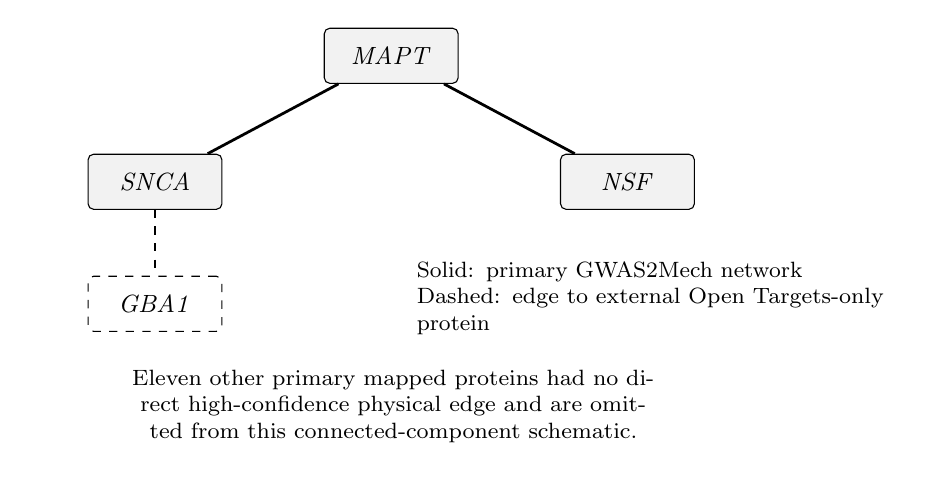
\begin{tikzpicture}[scale=1, every node/.style={font=\small}]
\node[draw,rounded corners=2pt,fill=gray!10,minimum width=1.7cm,minimum height=0.70cm] (mapt) at (0,0) {\textit{MAPT}};
\node[draw,rounded corners=2pt,fill=gray!10,minimum width=1.7cm,minimum height=0.70cm] (snca) at (-3,-1.6) {\textit{SNCA}};
\node[draw,rounded corners=2pt,fill=gray!10,minimum width=1.7cm,minimum height=0.70cm] (nsf) at (3,-1.6) {\textit{NSF}};
\node[draw,rounded corners=2pt,dashed,minimum width=1.7cm,minimum height=0.70cm] (gba) at (-3,-3.15) {\textit{GBA1}};
\draw[line width=1pt] (mapt)--(snca);
\draw[line width=1pt] (mapt)--(nsf);
\draw[line width=0.9pt,dashed] (snca)--(gba);
\node[align=left,text width=6cm,anchor=west,font=\footnotesize] at (0.2,-3.08) {Solid: primary GWAS2Mech network\\Dashed: edge to external Open Targets-only protein};
\node[align=center,text width=9cm,font=\footnotesize] at (0,-4.45) {Eleven other primary mapped proteins had no direct high-confidence physical edge and are omitted from this connected-component schematic.};
\end{tikzpicture}
\caption{Schematic of the directly connected seed proteins at STRING physical confidence $\geq 0.700$. The solid edges (\textit{MAPT}--\textit{SNCA}, \textit{MAPT}--\textit{NSF}) are the two primary GWAS2Mech-only associations; the dashed \textit{SNCA}--\textit{GBA1} association appears only when the external Open Targets seed is included. This simplified diagram is derived from the network summary and does not depict all isolated nodes or the expanded connector network.}
\label{fig:step15_primary_physical}
\end{figure}

\subsubsection{Excess protein-association connectivity}
Despite the sparseness of the primary physical-only graph, STRING's distinct PPI-enrichment test reported 12 observed protein-association edges, compared with approximately one expected edge under its organism-level reference distribution, for the 14 mapped primary proteins ($P=1.92\times10^{-11}$; BH-adjusted $q=5.76\times10^{-11}$). The 19-gene prior-robust set yielded 12 mapped proteins and 11 observed edges, compared with an expected count reported as zero after rounding ($P=6.26\times10^{-12}$; BH-adjusted $q=3.76\times10^{-11}$). The six tests and their corrected results are summarised in Table~\ref{tab:step15_ppi_enrichment}. In these results, the expected edge counts are output-rounded values and should not be used to calculate a precise fold enrichment when zero is printed.

\begin{table}[!htbp]
\centering\scriptsize
\caption{STRING PPI-enrichment analysis with BH correction across six tested gene sets. The PPI endpoint measures excess association connectivity in STRING and is distinct from the direct physical graph. Comparison groups retain their upstream Step~14 membership definitions; groups named \texttt{CORE\_STRONG\_OT\_*} are not guaranteed to be strict disjoint subsets of the 24-gene \texttt{CORE\_STRONG} set.}
\label{tab:step15_ppi_enrichment}
\begin{tabularx}{\linewidth}{@{}Xrrrrr@{}}
\toprule
Gene set & Input & Mapped & Edges & $P$ & BH $q$ \\\midrule
\texttt{CORE\_STRONG} & 24 & 14 & 12 & $1.92\times10^{-11}$ & $5.76\times10^{-11}$ \\
\texttt{CORE\_STRONG\_PRIOR\_ROBUST} & 19 & 12 & 11 & $6.26\times10^{-12}$ & $3.76\times10^{-11}$ \\
\texttt{LOCUS\_TOP\_STRONG} & 7 & 6 & 0 & 1.00 & 1.00 \\
\texttt{CORE\_STRONG\_OT\_SUPPORTED} & 8 & 8 & 3 & $2.66\times10^{-5}$ & $5.32\times10^{-5}$ \\
\texttt{CORE\_STRONG\_OT\_DISCORDANT} & 18 & 8 & 3 & $1.20\times10^{-3}$ & $1.80\times10^{-3}$ \\
\texttt{OPEN\_TARGETS\_TOP1} & 6 & 6 & 2 & $3.60\times10^{-3}$ & $4.32\times10^{-3}$ \\
\bottomrule
\end{tabularx}
\end{table}

Excess STRING connectivity suggests that the subset of mapped candidate proteins is functionally associated within the existing STRING evidence system. It does not validate a disease mechanism independently, because STRING draws on overlapping sources of functional and pathway annotation and because the selected proteins include several genes from the complex chromosome~17 region. Furthermore, the tested genes were prioritised using molecular colocalisation rather than random sampling of the full protein-coding genome; organism-level STRING enrichment is therefore best considered supportive, exploratory network evidence rather than a primary causal statistic.

\subsubsection{Network centrality and connector-protein findings}
In the \emph{primary} physical graph, \textit{MAPT} had the highest degree (2; connected to \textit{SNCA} and \textit{NSF}); these latter proteins each had degree~1. The other 11 mapped primary proteins were isolated at the chosen physical-association threshold. Thus, the strongest primary result was a small three-protein component rather than a broadly interconnected 14-protein mechanism.

In the expanded \emph{combined-seed} physical graph, \textit{MAPT} became the most connected and highest-betweenness input protein (degree 13; betweenness 0.3613), followed by \textit{SNCA} (degree 8; betweenness 0.2437). External \textit{GBA1} had degree 3. \textit{GAK} and \textit{GCH1}, although isolated in the primary direct physical graph, each gained one predicted physical association after expansion. These changes reflect database-added proteins and should not be interpreted as increased GWAS or colocalisation support for those genes.

\begin{table}[!htbp]
\centering\small
\caption{Selected nodes in the 36-node expanded physical network. Connector nodes were added algorithmically by STRING and are not part of the primary GWAS2Mech gene set unless separately indicated.}
\label{tab:step15_hubs}
\begin{tabular}{@{}llrrr@{}}
\toprule
Protein & Node class & Degree & Betweenness & PageRank \\\midrule
\textit{MAPT} & GWAS2Mech & 13 & 0.36135 & 0.21261 \\
\textit{SNCA} & GWAS2Mech + OT & 8 & 0.24370 & 0.12793 \\
\textit{GBA1}/GBA & OT-only & 3 & 0.07059 & 0.04622 \\
\textit{DNAJC6} & Connector & 2 & 0.03697 & 0.03868 \\
\textit{NSF} & GWAS2Mech & 2 & 0.03697 & 0.03841 \\
\textit{SYN1} & Connector & 2 & 0 & 0.03060 \\
\textit{GCH1} & GWAS2Mech & 1 & 0 & 0.03636 \\
\textit{GAK} & GWAS2Mech + OT & 1 & 0 & 0.02353 \\
\bottomrule
\end{tabular}
\end{table}

Among 20 first-order connector proteins were \textit{DNAJC6}, \textit{SYN1}, \textit{SNCAIP}, \textit{TPPP}, \textit{SNCB}, \textit{GCHFR}, \textit{UGCG}, and \textit{GBA2}. \textit{DNAJC6} and \textit{SYN1} each contacted two seed proteins in the expanded graph; \textit{GCHFR} provided a connection to \textit{GCH1}, while \textit{GAK} was connected through an added protein. Seven connectors were flagged by the script as having a neighbour labelled GWAS2Mech strong and a neighbour labelled Open Targets top-ranked. This count must be interpreted cautiously: a single shared GWAS2Mech/OT seed may satisfy both labels, so the seven flagged connectors do not necessarily bridge two distinct groups of proteins. Connector nodes do not acquire GWAS, fine-mapping or molecular-QTL evidence through their network proximity.

\subsubsection{Integration with pathway findings and sensitivity analyses}
The Step~15 integration table covered the 90 significant primary pathway terms reported in Step~14, yielding 215 gene--pathway annotation rows. For each pathway, the analysis counted members of the primary gene set and the number of STRING physical edges among those members, and carried forward the previously calculated leave-one-gene-out and leave-one-region-out significance-retention fractions. Representative results are shown in Table~\ref{tab:step15_pathway_network}. The pathway P-values are inherited from Step~14; they are \emph{not} newly generated pathway P-values from the protein network. The Step~14 enrichment used an exploratory annotated-genome background rather than a complete molecular-QTL assay-eligible background, so these terms remain provisional.

\begin{table}[!htbp]
\centering\scriptsize
\caption{Selected Step~14 pathway terms contextualised with primary Step~15 physical-network edges. ``Physical edges'' are the number of edges within the \emph{primary GWAS2Mech} gene members of that pathway. Gene and region retention fractions correspond to separate Step~14 deletion sensitivity tests. No mechanistic direction was inferred.}
\label{tab:step15_pathway_network}
\begin{tabularx}{\linewidth}{@{}Xrrrrr@{}}
\toprule
Pathway/process & Step14 $q$ & Genes & Physical edges & Region LOO & Gene LOO \\\midrule
Secretase involvement in neurodegenerative diseases & 0.002152 & 2 & 1 & 4/6 & 22/24 \\
Synaptic vesicle recycling & 0.003226 & 3 & 0 & 4/6 & 23/24 \\
Synaptic vesicle endocytosis & 0.003226 & 3 & 0 & 4/6 & 23/24 \\
Dopamine biosynthetic process & 0.003226 & 2 & 0 & 4/6 & 22/24 \\
Cellular response to chemical stress & 0.003226 & 4 & 1 & 5/6 & 23/24 \\
Macrophage activation & 0.003226 & 3 & 1 & 5/6 & 23/24 \\
Cellular response to oxidative stress & 0.009786 & 3 & 1 & 5/6 & 23/24 \\
Microglial cell activation & 0.009786 & 2 & 1 & 4/6 & 22/24 \\
\bottomrule
\end{tabularx}
\end{table}

The zero primary physical-edge counts for synaptic vesicle recycling, synaptic vesicle endocytosis and dopamine biosynthesis do not invalidate those gene-set annotations: participating proteins may be connected indirectly, have context-specific interactions, or influence a common process without detectable physical binding at this threshold. Conversely, a shared network edge is not independent experimental validation of a gene-to-pathway causal effect. The gene--pathway export explicitly records pathway direction as \texttt{UNKNOWN\_NOT\_TESTED}.

\subsubsection{Interpretation, quality-control caveats, and the next mechanistic stage}
The key result of Step~15 was the combination of significant organism-background STRING protein-association enrichment among mapped high-confidence candidates and a relatively sparse primary high-confidence physical-association graph. A core \textit{MAPT}--\textit{SNCA}--\textit{NSF} connected component was identifiable directly from primary GWAS2Mech proteins; the \textit{SNCA}--\textit{GBA1} edge and additional biological connectors emerged in comparator-inclusive or expanded network analyses. The most central nodes of the expanded physical graph, particularly \textit{MAPT} and \textit{SNCA}, are coherent with the neuronal/proteostasis themes of Step~14, but centrality and proximity do not demonstrate causal mediation of Parkinson's disease.

Interpretation requires attention to the following audit findings. First, 10/24 primary candidates were non-protein-coding and could not be assessed as proteins in a standard STRING PPI network. Second, STRING's physical network includes inferred physical associations and was not cross-validated against BioGRID in this run. Third, the output contains a preliminary \textit{LINC02210} symbol-based protein mapping that was subsequently excluded by the biotype audit; protein mapping must always be interpreted jointly with biotype. Fourth, the upstream secondary OT-supported and OT-discordant gene sets are not necessarily disjoint subsets of the 24 primary genes: for example, \textit{TMEM175} was present in an OT-supported secondary set but was not part of the 24 primary genes. Fifth, chromosome~17 contributes many colocalisation candidates and can influence both apparent functional connectivity and pathway enrichment. Finally, neither STRING confidence scores nor the network topology reveal whether a candidate allele increases or decreases a gene's molecular activity or whether perturbing that gene changes a pathway in a particular tissue.

The workflow-step-15 tables therefore provide mechanistic context and an evidence audit rather than establishing causal effector genes. The generated \nolinkurl{Step15_Gene_Pathway_Handoff.tsv} preserved gene identifiers, biotypes, pathway memberships, colocalisation evidence, and sensitivity attributes for the subsequent perturbation analysis. Published genetic-perturbation and gene-expression experiments were then used to evaluate gene-to-pathway direction and context where data were available; untested relationships remained unresolved. The network analysis did not support drug or therapeutic-response inference.



% The superseded Reactome-only Step16 v2 manuscript section has been
% removed. Step16 v3 source-ID analysis begins below.

% ================================================================
% GWAS2Mech — Step16, Step17, mechanistic interpretation
% Data provenance: user's Bunya Step16 v3 / Step17 v3 terminal
% summaries and 14 FDR-filtered rows, plus previously supplied
% Step12/Step14 locus and gene summary tables.
%
% Required in your existing manuscript preamble:
% \usepackage{amsmath,amssymb,booktabs,longtable,array,pdflscape}
% \usepackage[T1]{fontenc}
% Optional: \usepackage{hyperref}
% References: merge the companion .bib file into your bibliography.
%
% TABLE AUDIT: The per-variant links below are ASSOCIATION-LEVEL
% information; none establishes shared causal variant direction.
% The KANSL1 study accession / per-study locus ID has NOT been
% recovered from the supplied terminal report, and is not invented.
% ================================================================

\subsection{Perturbation analysis of genetically prioritised pathways (workflow step 16)}
\label{sec:gwas2mech_step16}
\subsubsection{Rationale and experimental resources}
\label{subsec:step16_rationale}
The genome-wide association study (GWAS)-to-mechanism workflow sought to determine whether altering genetically prioritised candidate genes produced measurable downstream transcriptional responses in biological processes implicated by Parkinson's disease (PD) pathway enrichment. The experiment was not a permutation of GWAS variants or randomised disease labels. Rather, it was a secondary analysis of publicly available gene-perturbation single-cell expression datasets, followed by \emph{gene-set permutation}-based enrichment testing. This distinction matters because an expression-signature enrichment result does not directly estimate the risk conferred by a genetic allele.

The analysis used harmonised public single-cell perturbation resources available through scPerturb \cite{Peidli2024scPerturb}. Of 54 inspected \texttt{.h5ad} files, 54 were reported as readable, and eight of the 24 primary GWAS2Mech candidate genes had a usable annotated perturbation: \textit{NSF}, \textit{KANSL1}, \textit{GAK}, \textit{MAPT}, \textit{DGKQ}, \textit{IDUA}, \textit{ARL17A}, and \textit{SLC50A1}. These were represented in 22 gene--dataset contrasts, all completing the descriptive analysis. Genes without usable perturbation coverage were not classified as biologically inactive or as negative experimental findings.

\subsubsection{Transcriptional contrasts and gene-set permutation analysis}
\label{subsec:step16_methods}
The source analysis was \nolinkurl{Step16_Perturbation_Directional_Pathways.py}, version \nolinkurl{3.0.0-source-matched-gsea}. For each annotated gene--dataset contrast, cells carrying the target perturbation were compared with the dataset's identified control population. Where relevant metadata were available, control selection accounted for experimental context; nevertheless, equivalence of donor, guide design, perturbation efficiency, and independent biological replication was not established across all datasets. Selected expression matrices were inspected to determine whether their values appeared count-like. Count-like values were transformed as
\begin{equation}
  y_{ij}=\log_{2}\left(1+10^{4}\frac{x_{ij}}{\sum_{k}x_{ik}}\right),
  \label{eq:step16_cptt}
\end{equation}
where $x_{ij}$ denotes the recorded expression of gene $j$ in cell $i$. Other nonnegative matrices were analysed on their stored scale. Because expression-scale recognition was heuristic rather than independently checked against every original study's preprocessing, the transformed values should be interpreted cautiously.

For each measured gene $j$, the descriptive rank was the difference in group means:
\begin{equation}
  r_j=\overline{y}_{j,\,\mathrm{perturbed}}-\overline{y}_{j,\,\mathrm{control}}.
  \label{eq:step16_rank}
\end{equation}
Genes were ranked by $r_j$, and the GSEApy implementation of preranked gene-set enrichment analysis was applied to the full available source-specific gene-set libraries \cite{Subramanian2005GSEA}. The recorded default configuration used 500 gene-set permutations, random seed 42, and an eligible overlap of 10--500 measured genes per pathway. The actual submitted SLURM options should be retained alongside the publication code release. The test was \emph{not} a biological-replicate-aware test of differential expression: each guide or cell does not automatically represent an independent replicate.

The pathways were identified by their native source identifiers rather than by names alone. The recorded library inventory comprised \texttt{GO\_Biological\_Process\_2023} (5,407 library gene sets) and \texttt{WikiPathway\_2021\_Human} (622 library gene sets). Although KEGG support was implemented in the software, a successfully loaded KEGG library was not recorded in this run. Step~14 pathway membership originated from a different enrichment backend and potentially different annotation releases; identity of a GO or WikiPathways term does not guarantee identical gene membership between the two resources.

For every tested pathway, the pipeline recorded a normalised enrichment score (NES), the GSEApy gene-set permutation false-discovery-rate estimate ($q_{\mathrm{GSEA}}$), the leading-edge genes, the source ID, and the experimental cell context. Positive NES denotes enrichment of the pathway's measured genes toward the positive end of the perturbed-minus-control expression ranking; negative NES denotes enrichment toward the negative end. Neither sign establishes increased/decreased biochemical pathway activity or the direction of the PD risk allele. Reported $q_{\mathrm{GSEA}}=0.000000$ values are software estimates from a finite permutation run, \emph{not} literal zero false-discovery probability. To avoid overstating their precision, these are printed as ``0 (reported)'' in the tables.

\subsubsection{Experimental coverage and source-matched pathway mapping}
\label{subsec:step16_coverage}
The 22 completed contrasts yielded 58,627 exploratory pathway-response records. Step~16 reported 1,017 responses overlapping its Step~14 pathway handoff, of which 995 corresponded to GO Biological Process and 22 to WikiPathways; 63 unique Step~14 pathway IDs were experimentally tested, and 69 of the 90 terms provided to Step~16 were exactly mappable to the available library identities. No independent biological-replicate-level FDR was available for these contrasts. The matching results therefore describe observed transcriptional patterns, not replicated causal effects.

\begin{table}[!htbp]
\centering\small
\caption{Recorded Step~16 v3 analysis coverage. A tested pathway or enrichment row is not an independently validated molecular mechanism. The 90 Step~14 terms in the Step~16 handoff must not be confused with the 130 distinct significant pathway terms represented across the broader Step~17 evidence universe.}
\label{tab:step16_inventory}
\begin{tabular}{@{}lr@{}}
\toprule
Measure & Recorded result \\
\midrule
Prioritised genes & 24 \\
Primary genes with annotated perturbation data & 8 \\
Readable local perturbation files & 54 \\
Completed gene--dataset contrasts & 22 \\
All exploratory pathway-response records & 58,627 \\
Step~14 handoff terms assessed for mapping & 90 \\
Handoff terms with exact library identity mapping & 69 \\
Experimentally tested unique Step~14 IDs (Step~16 scope) & 63 \\
Matched pathway-response records in Step~16 & 1,017 \\
Independent biological-replicate FDR available & No \\
\bottomrule
\end{tabular}
\end{table}

\subsubsection{Exploratory responses passing the gene-set permutation filter}
\label{subsec:step16_filtered}
Fourteen pathway--perturbation records satisfied the exploratory software-reported $q_{\mathrm{GSEA}}<0.05$ filter. These records comprised 12 distinct GO Biological Process terms, two perturbed genes (nine \textit{NSF} responses and five \textit{KANSL1} responses), and six unique gene--dataset contrasts. Critically, the 14 responses did \emph{not} constitute 14 distinct causal mechanisms. Only one response represented the same gene that contributed to the Step~14 enrichment of the corresponding pathway: \textit{NSF} perturbation and Golgi vesicle transport (GO:0048193). The remaining 13 were transcriptional responses of the perturbed gene to a pathway it had not driven in the Step~14 enrichment, and were retained as separate, exploratory cross-layer observations.

\begin{landscape}
\begingroup
\footnotesize
\setlength{\tabcolsep}{3pt}
\begin{longtable}{@{}p{0.105\linewidth}p{0.275\linewidth}p{0.058\linewidth}p{0.085\linewidth}r r p{0.10\linewidth}r@{}}
\caption{All 14 reported Step~17 v3 gene-set-permutation-filtered experimental responses ($q_{\mathrm{GSEA}}<0.05$). \emph{Driver} means that the perturbed gene was also a Step~14 input gene contributing to enrichment of that specific pathway; \emph{response only} means that the gene perturbation was observed to change the pathway-associated transcriptional signature but the perturbed gene was not one of the Step~14 pathway drivers. Step~14 FDR and Step~16 GSEA FDR are different tests. The NSF study/locus shown is an illustrative gene-level genetic association, not a pathway-specific experiment or causal-variant assignment. \textit{KANSL1} study/locus IDs require confirmation from the full Step~12 export.}\label{tab:step16_all14}\\
\toprule
GO identifier & Biological process & Target & Cell model & NES & GSEA $q$ & Relationship & Step~14 $q$\\
\midrule
\endfirsthead
\multicolumn{8}{l}{\textit{Table \thetable\ continued}}\\
\toprule
GO identifier & Biological process & Target & Cell model & NES & GSEA $q$ & Relationship & Step~14 $q$\\
\midrule
\endhead
\midrule\multicolumn{8}{r}{\textit{Continued on next page}}\\
\endfoot
\bottomrule
\endlastfoot

\texttt{GO:0048193} & Golgi vesicle transport & \textit{NSF} & RPE1 & 2.569492 & 0 (reported) & \textbf{Driver} & 0.049256 \\

\texttt{GO:0045333} & Cellular respiration & \textit{KANSL1} & Jurkat & -2.294186 & 0 (reported) & Response only & 0.028473 \\

\texttt{GO:0007005} & Mitochondrion organisation & \textit{KANSL1} & K562 essential & -2.044825 & 0 (reported) & Response only & 0.030000 \\

\texttt{GO:0032271} & Regulation of protein polymerisation & \textit{NSF} & RPE1 & -1.876480 & 0.011921 & Response only & 0.033835 \\

\texttt{GO:0045333} & Cellular respiration & \textit{KANSL1} & HepG2 & -1.902643 & 0.012281 & Response only & 0.028473 \\

\texttt{GO:0031110} & Regulation of microtubule polymerisation/depolymerisation & \textit{KANSL1} & RPE1 & -1.883377 & 0.016303 & Response only & 0.021512 \\

\texttt{GO:0010959} & Regulation of metal-ion transport & \textit{NSF} & RPE1 & -1.797126 & 0.021023 & Response only & 0.028608 \\

\texttt{GO:1902903} & Regulation of supramolecular-fibre organisation & \textit{KANSL1} & RPE1 & -1.845246 & 0.021540 & Response only & 0.049941 \\

\texttt{GO:0031110} & Regulation of microtubule polymerisation/depolymerisation & \textit{NSF} & RPE1 & -1.776954 & 0.026621 & Response only & 0.021512 \\

\texttt{GO:0010038} & Response to metal ion & \textit{NSF} & RPE1 & -1.770956 & 0.028407 & Response only & 0.014243 \\

\texttt{GO:0031109} & Microtubule polymerisation/depolymerisation & \textit{NSF} & RPE1 & -1.769217 & 0.028646 & Response only & 0.027937 \\

\texttt{GO:0048545} & Response to steroid hormone & \textit{NSF} & RPE1 & -1.703010 & 0.046450 & Response only & 0.028473 \\

\texttt{GO:0051402} & Neuron apoptotic process & \textit{NSF} & RPE1 & -1.693790 & 0.048481 & Response only & 0.028280 \\

\texttt{GO:0019216} & Regulation of lipid metabolism & \textit{NSF} & HepG2 & 1.950397 & 0.049513 & Response only & 0.044943 \\

\end{longtable}
\endgroup
\end{landscape}

\noindent Of the filtered responses, the highest positive NES was observed for \textit{NSF} perturbation in retinal pigment epithelial (RPE1) cells and the Golgi vesicle transport process (NES $=+2.569492$; GSEA $q$ reported as 0). The same GO term had been enriched among the genetically prioritised genes (Step~14 FDR $=0.049256$), with \textit{NSF} and \textit{GAK} as contributing input genes. The reported Step~14 region leave-one-out significance fraction for this pathway was 0.50, underscoring dependence on specific genomic regions. In contrast, \textit{KANSL1} perturbation in Jurkat cells was accompanied by negative enrichment of the cellular-respiration signature (NES $=-2.294186$; GSEA $q$ reported as 0), and \textit{KANSL1} perturbation in K562 cells was accompanied by negative enrichment of mitochondrion organisation (NES $=-2.044825$; GSEA $q$ reported as 0). Neither \textit{KANSL1} response is a same-gene Step~14 pathway-driver replication for these terms.

The ``neuron apoptotic process'' term also passed the exploratory GSEA filter following \textit{NSF} perturbation in RPE1 cells (NES $=-1.693790$; $q_{\mathrm{GSEA}}=0.048481$). This result denotes enrichment of expression-ranked genes annotated to neuronal apoptosis; it does \emph{not} establish neuronal apoptosis, neuronal loss, or a protective effect in retinal pigment epithelial cells. Likewise, the ``cellular respiration'' and ``mitochondrion organisation'' transcriptional signatures are not direct measurements of oxygen-consumption rate, respiratory-chain activity, or mitochondrial morphology.

The 14 results were selected using FDR values reported within source-specific gene-set analyses for each contrast. They were not subjected to a single additional correction pooling all 58,627 reported pathway records, and overlap among GO terms can induce substantial dependence. Therefore the count of filtered rows must not be interpreted as an experiment-wise family of 14 independently validated discoveries.

\subsection{Integration of genetic, pathway, and perturbation evidence (workflow step 17)}
\label{sec:gwas2mech_step17}
\subsubsection{Data linkage, mechanism units, and classification}
\label{subsec:step17_methods}
Step~17, version \texttt{3.0.0-step16v3-source-id-mechanisms}, integrated molecular association evidence (Step~12), Open Targets comparisons (Step~13), gene-set prioritisation and enrichment (Step~14), protein-association evidence (Step~15), and the experimental pathway responses (Step~16). The underlying analytical unit was \emph{pathway--candidate gene--experimental context}, rather than a claim that each output row represented an independent underlying disease mechanism. Study accession, locus identifier, candidate GWAS and molecular-QTL signal variants, colocalisation posterior, molecular phenotype, pathway driver status, interaction-network evidence, and perturbation response were retained in separate auditable tables and integrated in the mechanism master.

Only pathway records with the same \emph{source and native identifier} were linked; GO Biological Process terms were not equated with Reactome or WikiPathways terms because of similar names. Genetic association, annotated pathway membership, and observed perturbation response were also treated as three distinct propositions. A perturbation of a prioritised gene could yield an expression response for a pathway of which it was \emph{not} a Step~14 contributing gene; such responses were retained, but explicitly labelled \texttt{PERTURBATION\_RESPONSE\_ONLY\_NO\_STEP14\_MEMBERSHIP}. Conversely, a gene with no matched experimental response remained an unresolved hypothesis rather than a negative result.

The provisional mechanistic-evidence tiers comprised MT1, unresolved gene--pathway relationship; MT2, exploratory experimental pathway response; MT3, replicate-supported experimental pathway response; and MT4, directionally integrated genetic--molecular--experimental evidence satisfying additional consistency requirements. These tiers are rules describing evidence completeness, not statistically calibrated probabilities of gene causality, clinical intervention efficacy, or patient outcome.

For the present dataset, the programme did not establish allele-harmonised GWAS/QTL effect directions, independently validated perturbation target engagement, or replicate-aware experimental FDR. Therefore an MT2 classification does not establish increased or decreased disease risk through the given pathway, and no MT3 or MT4 designations were supported.

\subsubsection{Summary of integrated evidence}\label{subsec:step17_coverage}
Step~17 retained 130 unique significant pathway terms across its wider Step~14 enrichment outputs and 395 ranked genes, including 24 primary candidates. Eleven genes had pathway membership in the integrated pathway inventory. The integrated master contained 1,834 candidate gene--pathway--experimental-context records, comprising 1,602 MT2 exploratory records and 232 MT1 unresolved records; no MT3 or MT4 records were assigned. Step~17 reported 95 unique matched pathway identifiers and eight genes represented in experimental records. The difference between the Step~16 handoff count of 63 unique tested Step~14 IDs and the Step~17 total of 95 matched IDs reflects different source/pathway universes and requires a dedicated reconciliation audit rather than being treated as independent additional experiments.

\begin{table}[!htbp]
\centering\small
\caption{Recorded Step~17 v3 evidence inventory. Experimental records are repeated across pathways, genes and cell contexts; none of the row counts is a count of independent validated causal mechanisms.}
\label{tab:step17_inventory}
\begin{tabular}{@{}lr@{}}\toprule
Measure & Recorded result\\\midrule
Significant unique pathway terms in Step~17 & 130\\
Ranked gene identifiers & 395\\
Primary strong prioritised genes & 24\\
Genes with pathway membership in integrated records & 11\\
Candidate pathway--gene--context rows & 1,834\\
MT1 unresolved rows & 232\\
MT2 descriptive experimental rows & 1,602\\
MT3 replicate-supported rows & 0\\
MT4 directionally integrated rows & 0\\
Unique Step~17 matched pathway identifiers & 95\\
Unique experimentally represented genes & 8\\
Filtered $q_{\mathrm{GSEA}}<0.05$ records (this analysis) & 14\\
\bottomrule\end{tabular}
\end{table}

\subsubsection{Locus-to-gene support for the principal perturbation candidates}
\label{subsec:step17_variant_linkage}
The strongest same-gene cross-layer example was \textit{NSF} and Golgi vesicle transport. In the Step~12-derived locus--gene report, \textit{NSF} (ENSG00000073969) had its highest displayed colocalisation support in GWAS study \texttt{GCST90319903}, locus \texttt{L006}, where a candidate GWAS signal variant \texttt{17:46042921:A:AT} was paired with a molecular-QTL signal variant \texttt{17:46255593:C:T} for an \textit{NSF}-related isoform QTL in minor salivary gland ($PP_{H4}=0.934678$). These two displayed variants are \emph{representatives of GWAS and molecular association signals}, not necessarily the same SNP and not proven to be the shared causal allele. The same study/locus report listed an annotated high-PIP variant \texttt{17:46053470:CA:C}, classified as an intronic variant and annotated to \textit{KANSL1}; this locus-level annotation must not be erroneously described as an \textit{NSF} coding mutation or as the variant proven to explain its perturbation response. Additional \textit{NSF} locus-specific molecular associations were available but had lower displayed $PP_{H4}$ (Table~\ref{tab:step17_nsf_loci}).

\textit{KANSL1} (ENSG00000120071) was independently prioritised among the 24 strong genes. Its workflow-step-14 gene-ranking output recorded a maximum displayed $PP_{H4}=0.999985$, with an additional molecular-QTL signal labelled as an sQTL in posterior cingulate cortex. Both displayed GWAS and QTL signal identifiers were \texttt{17:45969671:T:A}. The available gene-ranking export did not contain the per-study GWAS accession, locus identifier, molecular-effect allele, functional consequence, or direction of the splice change; Table~\ref{tab:step17_variant_examples} therefore marks these fields as \emph{not verified}. The colocalisation posterior alone cannot establish that \textit{KANSL1} perturbation causes the mitochondrial or respiratory signatures observed in non-neuronal cells.

\begin{landscape}
\begingroup\footnotesize\setlength{\tabcolsep}{3pt}
\begin{longtable}{@{}p{0.13\linewidth}p{0.065\linewidth}p{0.17\linewidth}p{0.17\linewidth}r p{0.09\linewidth}p{0.13\linewidth}@{}}
\caption{All five available study-specific \textit{NSF} locus--gene records. Variant strings denote candidate GWAS or QTL signal representatives (genome coordinates with alleles), not verified causal variants or harmonised risk alleles. Locus identifiers are study-specific and must be interpreted with their GWAS accession. $PP_{H4}$ quantifies colocalisation support for a shared statistical signal under the adopted model; it is not the posterior probability that \textit{NSF} is the sole causal effector.}\label{tab:step17_nsf_loci}\\
\toprule
GWAS accession & Locus & GWAS signal variant & Molecular-QTL signal variant & $PP_{H4}$ & Modality & Reported molecular context \\
\midrule\endfirsthead
\toprule GWAS accession & Locus & GWAS signal variant & Molecular-QTL signal variant & $PP_{H4}$ & Modality & Reported context \\
\midrule\endhead
\bottomrule\endlastfoot
\texttt{GCST90319903} & L006 & \texttt{17:46042921:A:AT} & \texttt{17:46255593:C:T} & 0.934678 & isoQTL & Minor salivary gland\\
\texttt{GCST90476961} & L004 & \texttt{17:45854763:C:T} & \texttt{17:45846971:A:C} & 0.606696 & isoQTL & Muscle\\
\texttt{GCST90475830} & L004 & \texttt{17:45726951:A:G} & \texttt{17:45846971:A:C} & 0.397978 & isoQTL & Muscle\\
\texttt{GCST90473307} & L008 & \texttt{17:45616172:G:T} & \texttt{17:45606843:C:G} & 0.203940 & eQTL & Testis\\
\texttt{GCST90042681} & L002 & \texttt{17:46722744:G:A} & \texttt{17:46722744:G:A} & 0.075780 & pQTL & Parahippocampal gyrus\\
\end{longtable}\endgroup
\end{landscape}

\begin{table}[!htbp]
\centering\footnotesize
\caption{Representative gene- and locus-level variant evidence linked to the filtered perturbation results. Values reproduce the supplied Step~12/14 outputs; variant-to-gene assignment, study-specific locus identifier, allelic effect direction, and clinical consequence require independent reconciliation before causal inference. ``Region annotation'' is not synonymous with gene-specific effect annotation.}
\label{tab:step17_variant_examples}
\begin{tabular}{@{}p{0.13\linewidth}p{0.23\linewidth}p{0.24\linewidth}p{0.30\linewidth}@{}}
\toprule
Perturbed gene & Genetic context & Candidate variant & Annotation / important caveat\\\midrule
\textit{NSF} & \texttt{GCST90319903}/L006; isoQTL, minor salivary gland; $PP_{H4}=0.934678$ & GWAS: \texttt{17:46042921:A:AT}; QTL: \texttt{17:46255593:C:T} & Signal-level variants only; allelic orientation and disease-risk molecular direction unknown.\\
\textit{NSF} & Same GWAS locus; independent regional functional-annotation summary & Top regional PIP: \texttt{17:46053470:CA:C} & Intronic variant annotated to \textit{KANSL1}, not an established \textit{NSF} causal mutation. Gene-overlapping \textit{NSF} maximum PIP shown as 0 in this particular locus summary.\\
\textit{KANSL1} & Strong Step~14 gene ranking; sQTL in posterior cingulate cortex; max $PP_{H4}=0.999985$ & Reported GWAS/QTL representative: \texttt{17:45969671:T:A} & Gene-level ranking excerpt only; study accession, locus ID, specific splicing event and signed molecular effect require Step~12 verification.\\
\bottomrule
\end{tabular}
\end{table}


\subsubsection{Cross-layer audit of the 14 filtered response records}
\label{subsec:step17_crosslayer}
To provide a direct clinical audit from the pathway-level response to the locus-level association, Table~\ref{tab:step17_all14_linked} repeats each of the 14 filtered gene--pathway--experiment contexts with the \emph{best available gene-level genetic association}. This does not imply that an experimental gene-set response has been connected to a unique causal variant. A study-specific variant selected in a statistical colocalisation output is not interchangeable with the experimentally edited target, and a gene's strongest reported locus evidence must not be counted repeatedly as independent GWAS replications when several GO terms respond to the same perturbation.
\begin{landscape}
\begingroup\scriptsize\setlength{\tabcolsep}{2.5pt}
\begin{longtable}{@{}p{0.105\linewidth}p{0.075\linewidth}p{0.08\linewidth}p{0.135\linewidth}p{0.14\linewidth}p{0.14\linewidth}p{0.07\linewidth}p{0.145\linewidth}@{}}
\caption{Cross-layer audit of all 14 exploratory perturbation records, linking source-native pathway IDs to representative \emph{gene-level} GWAS/QTL evidence. NSF evidence is from the Step~12 study/locus table; KANSL1 is from the Step~14 \emph{gene-level summary only}. The genetic evidence is repeated across multiple pathway-response rows solely to aid traceability. A missing exact study/locus assignment is explicitly marked ``not verified''. No row demonstrates allele-harmonised causal mediation.}
\label{tab:step17_all14_linked}\\
\toprule
GO ID & Target & Experiment & Genetic accession/locus & Candidate GWAS variant & Candidate QTL variant & Gene best $PP_{H4}$ & Molecular evidence / caveat\\
\midrule\endfirsthead
\toprule GO ID & Target & Experiment & Accession/locus & GWAS signal & QTL signal & $PP_{H4}$ & Molecular evidence\\
\midrule\endhead
\bottomrule\endlastfoot
\texttt{GO:0048193} & \textit{NSF} & RPE1 & \texttt{GCST90319903}/L006 & \texttt{17:46042921:A:AT} & \texttt{17:46255593:C:T} & 0.934678 & isoQTL; minor salivary gland; allelic direction unknown \\
\texttt{GO:0045333} & \textit{KANSL1} & Jurkat & Not verified & \texttt{17:45969671:T:A} & \texttt{17:45969671:T:A} & 0.999985 & sQTL; posterior cingulate cortex; per-study locus and sign unresolved \\
\texttt{GO:0007005} & \textit{KANSL1} & K562 & Not verified & \texttt{17:45969671:T:A} & \texttt{17:45969671:T:A} & 0.999985 & sQTL; posterior cingulate cortex; per-study locus and sign unresolved \\
\texttt{GO:0032271} & \textit{NSF} & RPE1 & \texttt{GCST90319903}/L006 & \texttt{17:46042921:A:AT} & \texttt{17:46255593:C:T} & 0.934678 & isoQTL; minor salivary gland; allelic direction unknown \\
\texttt{GO:0045333} & \textit{KANSL1} & HepG2 & Not verified & \texttt{17:45969671:T:A} & \texttt{17:45969671:T:A} & 0.999985 & sQTL; posterior cingulate cortex; per-study locus and sign unresolved \\
\texttt{GO:0031110} & \textit{KANSL1} & RPE1 & Not verified & \texttt{17:45969671:T:A} & \texttt{17:45969671:T:A} & 0.999985 & sQTL; posterior cingulate cortex; per-study locus and sign unresolved \\
\texttt{GO:0010959} & \textit{NSF} & RPE1 & \texttt{GCST90319903}/L006 & \texttt{17:46042921:A:AT} & \texttt{17:46255593:C:T} & 0.934678 & isoQTL; minor salivary gland; allelic direction unknown \\
\texttt{GO:1902903} & \textit{KANSL1} & RPE1 & Not verified & \texttt{17:45969671:T:A} & \texttt{17:45969671:T:A} & 0.999985 & sQTL; posterior cingulate cortex; per-study locus and sign unresolved \\
\texttt{GO:0031110} & \textit{NSF} & RPE1 & \texttt{GCST90319903}/L006 & \texttt{17:46042921:A:AT} & \texttt{17:46255593:C:T} & 0.934678 & isoQTL; minor salivary gland; allelic direction unknown \\
\texttt{GO:0010038} & \textit{NSF} & RPE1 & \texttt{GCST90319903}/L006 & \texttt{17:46042921:A:AT} & \texttt{17:46255593:C:T} & 0.934678 & isoQTL; minor salivary gland; allelic direction unknown \\
\texttt{GO:0031109} & \textit{NSF} & RPE1 & \texttt{GCST90319903}/L006 & \texttt{17:46042921:A:AT} & \texttt{17:46255593:C:T} & 0.934678 & isoQTL; minor salivary gland; allelic direction unknown \\
\texttt{GO:0048545} & \textit{NSF} & RPE1 & \texttt{GCST90319903}/L006 & \texttt{17:46042921:A:AT} & \texttt{17:46255593:C:T} & 0.934678 & isoQTL; minor salivary gland; allelic direction unknown \\
\texttt{GO:0051402} & \textit{NSF} & RPE1 & \texttt{GCST90319903}/L006 & \texttt{17:46042921:A:AT} & \texttt{17:46255593:C:T} & 0.934678 & isoQTL; minor salivary gland; allelic direction unknown \\
\texttt{GO:0019216} & \textit{NSF} & HepG2 & \texttt{GCST90319903}/L006 & \texttt{17:46042921:A:AT} & \texttt{17:46255593:C:T} & 0.934678 & isoQTL; minor salivary gland; allelic direction unknown \\
\end{longtable}\endgroup
\end{landscape}


\subsubsection{Criteria for linking genetic and perturbation directions}
\label{subsec:step17_direction}
For each pathway--gene--experiment record, directional integration would require (i) a quality-controlled and allele-harmonised GWAS effect estimate, including phenotype coding and the allele associated with increased disease risk; (ii) a signed molecular-QTL effect on a precisely defined phenotype, such as total expression, isoform usage, or splice-junction abundance; (iii) a verified direction and magnitude of experimental target perturbation; and (iv) a statistically supported downstream response measured in a comparable cell system. The identity of the GWAS and QTL lead variants alone, or a high colocalisation $PP_{H4}$, does not satisfy these requirements. An isoQTL/sQTL effect cannot be rewritten as an increase or decrease in total gene expression without the appropriate molecular-phenotype definition.

Furthermore, a positive or negative NES is the sign of the \emph{transcriptional ranking} relative to pathway membership. It is not automatically a positive or negative sign for pathway enzymatic activity, clinical disease progression, or drug benefit. Given the absent independent replicate-level differential-expression estimates and unverified molecular/target directions, all filtered responses remained exploratory MT2 evidence. The classification is therefore properly interpreted as \emph{mechanistic hypothesis support} rather than confirmation of a complete causal chain.

 % ================================================================
% GWAS2Mech: FINAL LINKED MECHANISM TABLES (Step16 v3 / Step17 v3)
% Final Step17 evidence tables, inserted before the Discussion.
% Requires: booktabs, longtable, array, pdflscape
% M01--M14 are DISPLAY identifiers, not original MECH hashes.
% Empty cells = insufficient source evidence; NOT a negative result.
% ================================================================

\subsubsection{Final pathway-to-GWAS and perturbation evidence tables}
\label{subsec:step17_final_clinical_tables}

For clinical interpretability, Tables~\ref{tab:step17_final_gwas_pathway}
and~\ref{tab:step17_final_mechanisms} provide a two-part audit of the
14 exploratory response records filtered at the software-reported
$ q_{\mathrm{GSEA}}<0.05 $ threshold. Both tables share the local display
identifiers M01--M14; the identifiers denote \emph{gene--pathway--cell-context
observations}, not 14 independent causal mechanisms. Table~\ref{tab:step17_final_gwas_pathway}
shows the representative genetic association and pathway enrichment for
each observation, whereas Table~\ref{tab:step17_final_mechanisms} shows
its perturbational expression signature and the unresolved links in the
proposed causal chain. The Step~12 genetic association is intentionally
repeated when one gene has several experimental pathway responses.

\begin{landscape}
\begingroup\scriptsize\setlength{\tabcolsep}{1pt}
\renewcommand{\arraystretch}{1.18}
\begin{longtable}{@{}Y{0.040\linewidth}Y{0.225\linewidth}Y{0.125\linewidth}Y{0.225\linewidth}Y{0.280\linewidth}r@{}}
\caption{Final \emph{GWAS-to-pathway evidence table} for all 14 exploratory gene--pathway--experiment observations. Each row shows the Step~14 pathway and the best available \emph{gene-level representative} association. The same NSF study/locus is repeated for distinct experimental responses; these are not independent GWAS discoveries. Blank cells are unavailable or unverified, not negative findings.}
\label{tab:step17_final_gwas_pathway}\\
\toprule
\textbf{ID} & \textbf{Pathway / GO ID} & \makecell[l]{\textbf{Gene and GWAS}\\\textbf{study/locus}} & \textbf{Candidate signal variants} & \textbf{QTL and annotation} & \textbf{Step14 $q$}\\
\midrule\endfirsthead
\multicolumn{6}{l}{\textit{GWAS--pathway table continued}}\\
\toprule\textbf{ID} & \textbf{Pathway / GO ID} & \textbf{Gene; study/locus} & \textbf{GWAS and QTL signals} & \textbf{Molecular QTL / annotation} & \textbf{$q_{14}$}\\
\midrule\endhead
\midrule\multicolumn{6}{r}{\textit{Continued on next page}}\\\endfoot
\bottomrule\endlastfoot
M01 & Golgi vesicle transport\newline\texttt{GO:0048193} & \textit{NSF}\newline\texttt{GCST90319903}/L006 & GWAS: \texttt{17:46042921:A:AT}\newline QTL: \texttt{17:46255593:C:T} & isoQTL, minor salivary gland; $PP_{H4}=0.934678$. Regional high-PIP annotation: intronic \textit{KANSL1}$^{a}$. & 0.049256 \\
M02 & Cellular respiration\newline\texttt{GO:0045333} & \textit{KANSL1}\newline & GWAS: \texttt{17:45969671:T:A}$^{b}$\newline QTL: \texttt{17:45969671:T:A}$^{b}$ & sQTL, posterior cingulate cortex; gene-level maximum $PP_{H4}=0.999985$.  & 0.028473 \\
M03 & Mitochondrion organisation\newline\texttt{GO:0007005} & \textit{KANSL1}\newline & GWAS: \texttt{17:45969671:T:A}$^{b}$\newline QTL: \texttt{17:45969671:T:A}$^{b}$ & sQTL, posterior cingulate cortex; gene-level maximum $PP_{H4}=0.999985$.  & 0.030000 \\
M04 & Regulation of protein polymerisation\newline\texttt{GO:0032271} & \textit{NSF}\newline\texttt{GCST90319903}/L006 & GWAS: \texttt{17:46042921:A:AT}\newline QTL: \texttt{17:46255593:C:T} & isoQTL, minor salivary gland; $PP_{H4}=0.934678$. Regional high-PIP annotation: intronic \textit{KANSL1}$^{a}$. & 0.033835 \\
M05 & Cellular respiration\newline\texttt{GO:0045333} & \textit{KANSL1}\newline & GWAS: \texttt{17:45969671:T:A}$^{b}$\newline QTL: \texttt{17:45969671:T:A}$^{b}$ & sQTL, posterior cingulate cortex; gene-level maximum $PP_{H4}=0.999985$.  & 0.028473 \\
M06 & Regulation of microtubule\newline polymerisation/\allowbreak depolymerisation\newline\texttt{GO:0031110} & \textit{KANSL1}\newline & GWAS: \texttt{17:45969671:T:A}$^{b}$\newline QTL: \texttt{17:45969671:T:A}$^{b}$ & sQTL, posterior cingulate cortex; gene-level maximum $PP_{H4}=0.999985$.  & 0.021512 \\
M07 & Regulation of metal-ion transport\newline\texttt{GO:0010959} & \textit{NSF}\newline\texttt{GCST90319903}/L006 & GWAS: \texttt{17:46042921:A:AT}\newline QTL: \texttt{17:46255593:C:T} & isoQTL, minor salivary gland; $PP_{H4}=0.934678$. Regional high-PIP annotation: intronic \textit{KANSL1}$^{a}$. & 0.028608 \\
M08 & Regulation of\newline supramolecular-fibre organisation\newline\texttt{GO:1902903} & \textit{KANSL1}\newline & GWAS: \texttt{17:45969671:T:A}$^{b}$\newline QTL: \texttt{17:45969671:T:A}$^{b}$ & sQTL, posterior cingulate cortex; gene-level maximum $PP_{H4}=0.999985$.  & 0.049941 \\
M09 & Regulation of microtubule\newline polymerisation/\allowbreak depolymerisation\newline\texttt{GO:0031110} & \textit{NSF}\newline\texttt{GCST90319903}/L006 & GWAS: \texttt{17:46042921:A:AT}\newline QTL: \texttt{17:46255593:C:T} & isoQTL, minor salivary gland; $PP_{H4}=0.934678$. Regional high-PIP annotation: intronic \textit{KANSL1}$^{a}$. & 0.021512 \\
M10 & Response to metal ion\newline\texttt{GO:0010038} & \textit{NSF}\newline\texttt{GCST90319903}/L006 & GWAS: \texttt{17:46042921:A:AT}\newline QTL: \texttt{17:46255593:C:T} & isoQTL, minor salivary gland; $PP_{H4}=0.934678$. Regional high-PIP annotation: intronic \textit{KANSL1}$^{a}$. & 0.014243 \\
M11 & Microtubule\newline polymerisation/\allowbreak depolymerisation\newline\texttt{GO:0031109} & \textit{NSF}\newline\texttt{GCST90319903}/L006 & GWAS: \texttt{17:46042921:A:AT}\newline QTL: \texttt{17:46255593:C:T} & isoQTL, minor salivary gland; $PP_{H4}=0.934678$. Regional high-PIP annotation: intronic \textit{KANSL1}$^{a}$. & 0.027937 \\
M12 & Response to steroid hormone\newline\texttt{GO:0048545} & \textit{NSF}\newline\texttt{GCST90319903}/L006 & GWAS: \texttt{17:46042921:A:AT}\newline QTL: \texttt{17:46255593:C:T} & isoQTL, minor salivary gland; $PP_{H4}=0.934678$. Regional high-PIP annotation: intronic \textit{KANSL1}$^{a}$. & 0.028473 \\
M13 & Neuron apoptotic process\newline\texttt{GO:0051402} & \textit{NSF}\newline\texttt{GCST90319903}/L006 & GWAS: \texttt{17:46042921:A:AT}\newline QTL: \texttt{17:46255593:C:T} & isoQTL, minor salivary gland; $PP_{H4}=0.934678$. Regional high-PIP annotation: intronic \textit{KANSL1}$^{a}$. & 0.028280 \\
M14 & Regulation of lipid metabolism\newline\texttt{GO:0019216} & \textit{NSF}\newline\texttt{GCST90319903}/L006 & GWAS: \texttt{17:46042921:A:AT}\newline QTL: \texttt{17:46255593:C:T} & isoQTL, minor salivary gland; $PP_{H4}=0.934678$. Regional high-PIP annotation: intronic \textit{KANSL1}$^{a}$. & 0.044943 \\
\end{longtable}
\noindent\footnotesize
$^{a}$ The regional high-PIP variant is \texttt{17:46053470:CA:C}, annotated as intronic to
\textit{KANSL1}. It is \emph{not} the same as the displayed NSF GWAS or QTL representative and is not proven to cause the NSF perturbation response.
$^{b}$ KANSL1 variant identifiers derive from a gene-level signal summary; the associated study accession and locus ID were not independently verified. The reported gene-level maximum $PP_{H4}$ may not be attributable to every displayed molecular association.
Step14 $q$ and Step~16 GSEA $q$ are separate statistical measures. $PP_{H4}$ indicates support for a shared association signal under the colocalisation model, not confirmation of a gene-level causal mechanism.\par
\endgroup\end{landscape}

\begin{landscape}
\begingroup\scriptsize\setlength{\tabcolsep}{1.4pt}
\renewcommand{\arraystretch}{1.16}
\begin{longtable}{@{}Y{0.045\linewidth}Y{0.240\linewidth}Y{0.170\linewidth}Y{0.077\linewidth}Y{0.080\linewidth}Y{0.083\linewidth}Y{0.094\linewidth}Y{0.099\linewidth}Y{0.053\linewidth}@{}}
\caption{Final \emph{mechanism-by-mechanism experimental evidence} for all 14 exploratory Step~16/17 responses. M01--M14 are presentation identifiers, not 14 confirmed molecular mechanisms. ``Step14 driver'' is Yes only if the experimentally perturbed gene contributed to the genetic enrichment of this exact pathway. All displayed experiments passed the exploratory software-reported GSEA $q<0.05$ filter, \emph{not} a replicate-aware experimental test. Empty target-effect and risk-direction fields denote unavailable validation evidence.}
\label{tab:step17_final_mechanisms}\\
\toprule
\textbf{ID} & \textbf{Pathway / GO term} & \textbf{Gene; model} & \textbf{NES} & \textbf{GSEA $q$} & \makecell[l]{\textbf{Step14}\\\textbf{driver?}} & \makecell[l]{\textbf{Target effect}\\\textbf{verified?}} & \makecell[l]{\textbf{Risk direction}\\\textbf{aligned?}} & \textbf{Tier}\\
\midrule\endfirsthead
\multicolumn{9}{l}{\textit{Experimental evidence table continued}}\\
\toprule\textbf{ID} & \textbf{Pathway / GO term} & \textbf{Gene; model} & \textbf{NES} & \textbf{GSEA $q$} & \textbf{Driver?} & \makecell[l]{\textbf{Target}\\\textbf{verified?}} & \makecell[l]{\textbf{Risk}\\\textbf{aligned?}} & \textbf{Tier}\\
\midrule\endhead
\midrule\multicolumn{9}{r}{\textit{Continued on next page}}\\\endfoot
\bottomrule\endlastfoot
M01 & Golgi vesicle transport\newline\texttt{GO:0048193} & \textit{NSF}\newline RPE1 (RW22) & 2.569492 & 0$^{c}$ & Yes &  &  & MT2 \\
M02 & Cellular respiration\newline\texttt{GO:0045333} & \textit{KANSL1}\newline Jurkat (NO24) & -2.294186 & 0$^{c}$ & No &  &  & MT2 \\
M03 & Mitochondrion organisation\newline\texttt{GO:0007005} & \textit{KANSL1}\newline K562 essential (RW22) & -2.044825 & 0$^{c}$ & No &  &  & MT2 \\
M04 & Regulation of protein polymerisation\newline\texttt{GO:0032271} & \textit{NSF}\newline RPE1 (RW22) & -1.876480 & 0.011921 & No &  &  & MT2 \\
M05 & Cellular respiration\newline\texttt{GO:0045333} & \textit{KANSL1}\newline HepG2 (NO24) & -1.902643 & 0.012281 & No &  &  & MT2 \\
M06 & Regulation of microtubule\newline polymerisation/\allowbreak depolymerisation\newline\texttt{GO:0031110} & \textit{KANSL1}\newline RPE1 (RW22) & -1.883377 & 0.016303 & No &  &  & MT2 \\
M07 & Regulation of metal-ion transport\newline\texttt{GO:0010959} & \textit{NSF}\newline RPE1 (RW22) & -1.797126 & 0.021023 & No &  &  & MT2 \\
M08 & Regulation of\newline supramolecular-fibre organisation\newline\texttt{GO:1902903} & \textit{KANSL1}\newline RPE1 (RW22) & -1.845246 & 0.021540 & No &  &  & MT2 \\
M09 & Regulation of microtubule\newline polymerisation/\allowbreak depolymerisation\newline\texttt{GO:0031110} & \textit{NSF}\newline RPE1 (RW22) & -1.776954 & 0.026621 & No &  &  & MT2 \\
M10 & Response to metal ion\newline\texttt{GO:0010038} & \textit{NSF}\newline RPE1 (RW22) & -1.770956 & 0.028407 & No &  &  & MT2 \\
M11 & Microtubule\newline polymerisation/\allowbreak depolymerisation\newline\texttt{GO:0031109} & \textit{NSF}\newline RPE1 (RW22) & -1.769217 & 0.028646 & No &  &  & MT2 \\
M12 & Response to steroid hormone\newline\texttt{GO:0048545} & \textit{NSF}\newline RPE1 (RW22) & -1.703010 & 0.046450 & No &  &  & MT2 \\
M13 & Neuron apoptotic process\newline\texttt{GO:0051402} & \textit{NSF}\newline RPE1 (RW22) & -1.693790 & 0.048481 & No &  &  & MT2 \\
M14 & Regulation of lipid metabolism\newline\texttt{GO:0019216} & \textit{NSF}\newline HepG2 (NO24) & 1.950397 & 0.049513 & No &  &  & MT2 \\
\end{longtable}
\noindent\footnotesize
RW22: Replogle--Weissman 2022 screens; NO24: Nadig--O'Connor 2024 screens. Exact source filenames and target/control cell counts are retained in the Step~16 run audit. All rows had an exploratory response under the software-reported $q<0.05$ criterion (Yes); independent experimental significance is unknown. For the three entries where software printed $q=0.000000$, the superscript $c$ denotes a finite-permutation reported zero, not a zero false-discovery probability. Empty cells reflect unavailable verified target engagement and allele-harmonised direction, not negative experimental results. Every row is currently MT2.\par
\endgroup\end{landscape}

\noindent\textbf{Clinical interpretation.}
The only observation in this filtered set with a \emph{same-gene}
connection between Step~14 pathway enrichment and Step~16 perturbation
was M01 (\textit{NSF}--Golgi vesicle transport, RPE1). This result is
best considered a tractable experimental hypothesis, not evidence that
a specific Parkinson's disease risk allele alters Golgi transport in
patients. M02--M14 are measurable perturbation-related transcriptional
responses associated with genetically enriched pathway \emph{terms},
but the perturbed gene was not among the Step~14 enrichment drivers for
that exact term. Independent biological replication and allele-resolved
molecular effect direction remain necessary before promotion to a
validated mechanistic interpretation.





\section{Discussion}
\label{sec:gwas2mech_mechanistic_discussion}
\subsection{Principal finding and evidential scope}
\label{subsec:discussion_main}
Source-specific pathway-library matching recovered transcriptional perturbation evidence linked to the native identifiers of genetically implicated pathways. Reactome-only matching did not adequately cover the Gene Ontology-dominated pathway inventory from workflow step~14. With source-specific matching, 1,017 pathway-response records overlapped the workflow-step-14 handoff, and the final integration retained 1,602 exploratory gene--pathway--context records. These counts describe evidence integration rather than independent disease mechanisms. Of the 14 filtered responses in Table~\ref{tab:step16_all14}, only one involved a perturbed gene that also drove enrichment of the corresponding pathway, making it the most direct observed bridge between genetic prioritisation and perturbation response.

The study therefore supports three levels of interpretation: first, independently collected genetic/molecular association evidence prioritises candidate genes; second, curated gene-set over-representation associates subsets of those genes with biological processes; and third, perturbation datasets demonstrate whether experimentally changing selected genes is accompanied by a downstream expression signature for a particular process in a particular cell system. The outputs presently do not establish which variant modifies the gene in patients, whether the relevant molecular effect has the same direction as the experimental intervention, or whether the observed pathway signature mediates Parkinsonian neurodegeneration.

\subsection{Vesicular transport as the clearest same-gene candidate link}
\label{subsec:discussion_nsf}
The clearest integrated candidate signal involved \textit{NSF} and Golgi vesicle transport (GO:0048193). \textit{NSF} contributed to the Step~14 gene-set enrichment alongside \textit{GAK} (FDR $=0.049256$), and independent perturbation of \textit{NSF} was associated with a strong positive-ranked Golgi vesicle transport signature in RPE1 cells (NES $=+2.569492$; permutation FDR reported as 0). This observation is consistent with the broader biological relevance of vesicular trafficking to neuronal membrane and protein handling. Its evidential strength lies in the concordance of \emph{gene identity and pathway identity} across genetic annotation and functional perturbation; it does not imply that the GWAS association experimentally reproduces the perturbation or that Golgi trafficking is activated in patients.

Importantly, the Step~12 gene association supporting \textit{NSF} was principally an isoQTL colocalisation signal in minor salivary gland rather than a demonstrated disease-relevant dopaminergic neuron context. The representative GWAS signal and QTL signal variants differed, and the top regionally annotated high-PIP variant was intronic to \textit{KANSL1}. The broader chromosome~17q21.31 region includes complex haplotypic architecture and long-range linkage disequilibrium; fine-mapped markers and multiple neighbouring gene associations require particularly careful interpretation \cite{Bowles2022MAPTInversion}. Consequently, the RPE1 perturbation cannot be directly assigned to a specific PD risk allele at this locus. The next experimental test should link phased locus-level alleles to verified \textit{NSF} molecular changes and evaluate downstream vesicular-trafficking phenotypes in relevant neural models.

The cross-model comparison further limits broad generalisation. The source-matched Golgi signature for \textit{NSF} was not comparably supported in the reported iPSC-induced neuron experiment (NES $=-0.835779$, $q_{\mathrm{GSEA}}=0.956533$), and other cell lines displayed heterogeneous signs. This observation does not disprove a vesicle-trafficking mechanism; rather, it demonstrates that experimental model, assay, target engagement and transcriptional context are material to the interpretation. A targeted validation design should consider human dopaminergic neurons and other relevant disease-cell populations, multiple independent perturbation guides, and direct vesicle-trafficking readouts rather than expression-based enrichment alone.

\subsection{KANSL1-associated mitochondrial and cytoskeletal responses}
\label{subsec:discussion_kansl1}
A second prominent set of exploratory signatures followed perturbation of \textit{KANSL1}. A strongly negative-ranked cellular-respiration signature was recorded in Jurkat cells (NES $=-2.294186$, GSEA FDR reported as 0) and a separate negative-ranked mitochondrion organisation signature in K562 cells (NES $=-2.044825$, GSEA FDR reported as 0). A cellular-respiration signal was also observed in HepG2 cells (NES $=-1.902643$, $q_{\mathrm{GSEA}}=0.012281$), providing some cross-model support for a related transcriptional theme. These results suggest that experimentally altering \textit{KANSL1} can affect expression programmes annotated to respiration and mitochondrial biology in the analysed cell lines, but do not directly measure mitochondrial respiration, organelle integrity, mitochondrial membrane potential, or vulnerability to neurodegeneration.

The same-gene genetic pathway link is weaker than for the \textit{NSF}--Golgi example. Although \textit{KANSL1} itself was strongly genetically prioritised ($PP_{H4}^{\max}=0.999985$), it was \emph{not} among the input genes driving Step~14 enrichment of cellular respiration or mitochondrion organisation in the supplied pathway-driver report. Those Step~14 terms instead involved other genes, including \textit{SNCA} and external-comparator \textit{GBA1}. Thus, the \textit{KANSL1} signatures provide functional responses in a candidate GWAS-prioritised gene, but not a complete independent genetic-to-\textit{KANSL1}-to-mitochondria pathway proof. The Step~14 pathway enrichment was also sensitive to genomic-region exclusion: the reported leave-region-out significance fractions were 0 for cellular respiration and approximately 0.17 for mitochondrion organisation. Their potential relevance should therefore be tested with independent biological replicates and direct functional assays in patient-relevant cells.

Additional negative-ranked \textit{KANSL1} responses involved microtubule dynamics and supramolecular-fibre organisation in RPE1 cells. Together with the mitochondrial terms, these observations motivate experiments probing cytoskeletal organisation and organelle transport. They should not be construed as direct changes to microtubule assembly kinetics or axonal transport until protein- or imaging-based measurements corroborate the transcriptional observations.

\subsection{Other NSF responses: cytoskeleton, ion homeostasis and cell death}
\label{subsec:discussion_secondary}
The remaining \textit{NSF} responses below the exploratory GSEA threshold were mainly negative-ranked signatures concerning regulation of protein polymerisation, microtubule dynamics, response to metal ions, steroid-hormone response and the neuron-apoptotic-process ontology term in RPE1 cells, together with a positive-ranked regulation-of-lipid-metabolism signature in HepG2 cells. These observations are biologically heterogeneous and often describe overlapping GO annotations. Their coexistence is not equivalent to independent validation of multiple causal pathways, particularly as several nominally different terms can share genes from the same expression-ranked signature.

For example, the negative neuron-apoptotic-process signature (NES $=-1.693790$, $q_{\mathrm{GSEA}}=0.048481$) is a pathway \emph{expression-enrichment result} measured in retinal pigment epithelial cells; it does not demonstrate an anti-apoptotic effect, neuronal survival benefit, or treatment opportunity in patients. Similarly, terms involving ion transport do not report measured calcium or metal-ion flux, and steroid-hormone-response enrichment does not demonstrate endocrine receptor activation. These are candidates for mechanism-specific phenotyping only after replication and assay validation.

\subsection{Pathways without experimental closure}
\label{subsec:discussion_gaps}
Several biological processes relevant to Parkinson's disease were enriched among the genetically prioritised genes but lacked qualifying same-gene experimental responses in the filtered subset. These included dopamine biosynthesis (represented by \textit{GCH1} and \textit{SNCA} in the workflow-step-14 enrichment inventory), synaptic vesicle recycling (\textit{DGKQ}, \textit{SNCA}, and \textit{GAK}), and glial or microglial activation (including \textit{SNCA} and \textit{MAPT}). The analysed perturbation inventory contained no usable \textit{SNCA} or \textit{GCH1} contrasts. The absence of a functional response therefore reflects experimental coverage and pathway matching rather than evidence against a role in disease.

A clear reporting scheme should distinguish \emph{not assayed}, \emph{assayed but pathway not mapped}, \emph{assayed without exploratory significance}, \emph{exploratory response}, and \emph{replicate-validated response}. None of these categories alone demonstrates directional causal mediation. Data from non-neuronal or transformed cell lines should also remain distinct from neuron-specific Parkinson's disease evidence, even when a queried Gene Ontology term includes a neuron-related label.

\subsection{Statistical and genomic limitations}
\label{subsec:discussion_limits}
There are five key limitations. First, Step~14 pathway over-representation was performed on a selected and partly related set of GWAS-prioritised genes against an annotated-gene background, rather than an independently established full molecular-QTL-assay-eligible background. The sensitivity of the resulting pathway FDRs to that background should be established before publication-final pathway claims. Second, the 17q21.31 region can contribute correlated evidence for several nearby gene candidates because of structural haplotypes, complex linkage disequilibrium and overlapping molecular QTLs; neither multiple genes at one locus nor multiple related GWAS studies are equivalent to independent mechanistic replications. Third, Step~16's gene-set-permutation FDR does not reflect a full replicate-aware statistical test of the targeted perturbation in biological donors. False discoveries can arise from pseudoreplication in single-cell analyses if biological-level variation is ignored \cite{Squair2021FalseDiscoveries}. Fourth, gene-set versions from Step~14 and Step~16 were not guaranteed to have identical membership, even when the native pathway identifier was matched. Fifth, Step~17 lacks verified risk-associated molecular direction and experimentally verified target-effect direction, precluding inference of therapeutic benefit or causal mediation from NES signs alone.

A further reporting nuance is that Step~16 and Step~17 use different collections of upstream pathway terms: 90 handoff terms were available to the Step~16 run, whereas 130 unique significant pathway terms were represented in Step~17. The Step~16 scope yielded 63 tested Step~14 pathway identifiers from its 90-term handoff, while Step~17 matched 95 identifiers within a broader 130-term pathway universe. These figures have different denominators and therefore must not be subtracted or interpreted as independent biological discoveries. Whether every extra Step~17 identifier is traceable to a valid Step~16 experiment remains subject to a source-ID, gene-set-version and run-release audit before submission. This reconciliation is a provenance and integration-quality check, not evidence of either more or fewer independent mechanisms.

\subsection{Implications for experimental validation and clinical translation}
\label{subsec:discussion_next}
The principal translational value of these results is the creation of an auditable shortlist for experiments addressing explicitly identified evidence gaps. An appropriate validation programme would first confirm signed GWAS and molecular-QTL effects on harmonised alleles, including the precise molecular phenotype (total expression, isoform usage, splice junction or protein abundance), then test the corresponding increase or decrease in target function rather than assuming that all CRISPRi experiments mimic the risk allele. Cell-type-specific responses should be evaluated in appropriately differentiated human iPSC-derived dopaminergic neurons and, for immune-related mechanisms, relevant microglial or myeloid models. Independent biological donors or experimental replicates, multiple on-target guides, checks for target engagement and rescue experiments should be included where feasible. Replicate-aware expression analysis should precede confirmatory pathway testing; direct vesicle-trafficking, mitochondrial-function, cytoskeletal and neuronal-survival readouts would distinguish pathway-gene-expression signals from physiological mechanism.

The evidence tiers should therefore be described as provisional and contextual. MT1 records identify unresolved pathway--gene hypotheses; MT2 records document descriptive transcriptional responses; MT3 should require appropriate replicate-aware evidence; and MT4 should require independently supported, biologically interpretable concordance among the genetic allele, molecular effect, experimentally changed target and downstream pathway response. None of these categories by itself substitutes for human efficacy or safety evidence.

\section{Conclusions}\label{subsec:discussion_conclusion}
The source-identified integration of workflow steps 16 and 17 recovered exploratory transcriptional responses connected to genetically enriched pathways. The most direct same-gene candidate connection involved \textit{NSF} and Golgi vesicle transport. \textit{KANSL1} perturbations produced respiration-, mitochondrion-, and cytoskeleton-related transcriptional signatures, but \textit{KANSL1} was not a genetic enrichment driver for those specific pathway terms.

These findings narrow a broad GWAS-to-pathway inventory to concrete experimental hypotheses and show why cell context, source identity, and evidence provenance must remain explicit. The present data did not establish risk-allele-to-pathway causal direction, a disease-modifying intervention, or a clinically validated mechanism. GWAS2Mech should therefore be interpreted as a framework for genetically informed mechanistic hypothesis prioritisation with exploratory perturbation evidence.

\section*{Data and code availability}
\addcontentsline{toc}{section}{Data and code availability}
The analyses used public summary-level genetic, molecular-QTL, annotation, network, and perturbation resources identified in the resource tables and corresponding citations. The GWAS2Mech source code is available at \url{https://github.com/MuhammadMuneeb007/gwas2mech}. A versioned release, immutable commit identifier, and the derived analysis outputs should accompany the manuscript at submission to support exact reproduction.


\clearpage
\bibliographystyle{unsrtnat}
\bibliography{references}
\end{document}
